\chapter{Satellite Subsystems}
\label{ch:satellite_subsystems}
This section summarizes the main satellite subsystems and demonstrates that the mission architecture is technically feasible. Detailed design is not required, but preliminary analysis results should be presented.

\section{Electrical Power System}
\label{sec:electrical_power_system}
This section presents the preliminary Electrical Power System (EPS) analysis for the LINKU mission. The objective is to estimate the ideal solar power-generation capability of the satellite system, since the external geometry and available surface area impose direct constraints on the maximum power that can be generated by the solar panels. These estimates provide upper-bound power constraints for subsequent subsystem sizing.

The analysis is organized according to the satellite configurations associated with the mission operational stages: SAT-ABC, SAT-BC, and SAT-B and SAT-C at nominal maximum tether extension. For the EPS analysis, all configurations are simulated assuming a nadir-pointing attitude, in which the main longitudinal axis of each satellite configuration is aligned with the local nadir direction in the LVLH frame. COMSOL Multiphysics is used to estimate surface irradiation, thermal conditions, and available electrical power under representative orbital conditions.

\subsection{Power Generation Model and Conversion Methodology}
\label{sub:eps_power_generation_model}
The COMSOL simulations provide the incident surface irradiation on the satellite external surfaces. To estimate the available electrical power, the incident power is converted using representative solar-cell and system-level efficiency factors~\cite{Wertz2011SMAD, Solomon2025Electrical}. This conversion provides a preliminary estimate of the ideal solar power-generation capability for each configuration.

The generated electrical power, \(P_{\mathrm{elec}}(t)\), is estimated from the incident power, \(P_{\mathrm{in}}(t)\), as

\begin{equation}
P_{\mathrm{elec}}(t)
=
P_{\mathrm{in}}(t)
\eta_{\mathrm{cell}}
P_F
\eta_{\mathrm{sys}},
\label{eq:eps_electrical_power_conversion}
\end{equation}

where \(P_{\mathrm{in}}(t)\) is the total incident power on the active solar-panel surfaces, \(\eta_{\mathrm{cell}}\) is the solar-cell efficiency, \(P_F\) is the packing factor that accounts for inactive area on the mounting surfaces, and \(\eta_{\mathrm{sys}}\) accounts for system-level losses, including Maximum Power Point Tracking (MPPT) conversion losses, wiring losses, and thermal degradation.

For the preliminary EPS analysis, \(\eta_{\mathrm{cell}}\) is assumed to be in the range of \(28\%\)--\(30\%\), \(P_F\) is estimated as \(0.80\), and \(\eta_{\mathrm{sys}}\) is used to account for losses between the incident solar power and the usable electrical power available to the spacecraft subsystems.

\subsection{Computational Modeling and Orbital Geometry}
\label{sub:eps_computational_modeling_orbital_geometry}

The EPS analysis was implemented in COMSOL Multiphysics using the \textit{Orbital Thermal Loads} interface. The model was configured to evaluate the time-varying incident solar radiation on the satellite external surfaces, considering the orbital trajectory, spacecraft geometry, surface orientation, and thermo-optical properties of the selected faces.

The simulations were performed under representative Low Earth Orbit (LEO) conditions at an altitude of \(700~\mathrm{km}\). Two inclination cases were considered: a \(30^\circ\) prograde orbit and a \(94^\circ\) near-polar orbit. These cases are used to compare the effect of different illumination and eclipse conditions on the solar power-generation capability of the satellite configurations.

For the EPS analysis, mission operational stages with equivalent external power-generation geometry are grouped into three representative satellite configurations. These configurations determine the effective exposed area of the solar-panel surfaces and the possible self-shadowing conditions:

\begin{itemize}
    \item \textbf{SAT-ABC configuration:} This configuration represents the state in which SAT-A, SAT-B, and SAT-C are mechanically integrated and treated as a single external geometry for the EPS analysis. In this configuration, the external geometry of SAT-A defines the available surface area for solar power generation before the deployment of SAT-BC, as shown in Figure~\ref{fig:mesh_satabc}.

    \begin{figure}[H]
        \centering
        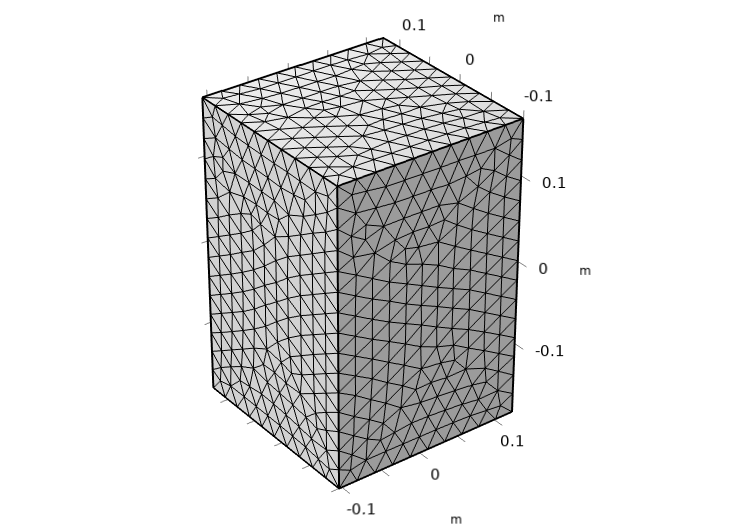
\includegraphics[width=0.5\textwidth]{INICTEL_Pictures/Mesh_SATA.png}
        \caption{Mesh geometry for the SAT-ABC configuration.}
        \label{fig:mesh_satabc}
    \end{figure}

    \item \textbf{SAT-BC configuration:} This configuration corresponds to the state after deployment from SAT-A and before SAT-B/SAT-C separation. In this state, SAT-B and SAT-C remain mechanically coupled and are modeled as a single rigid body for thermal and irradiation analysis, as shown in Figure~\ref{fig:mesh_satbc}.

    \begin{figure}[H]
        \centering
        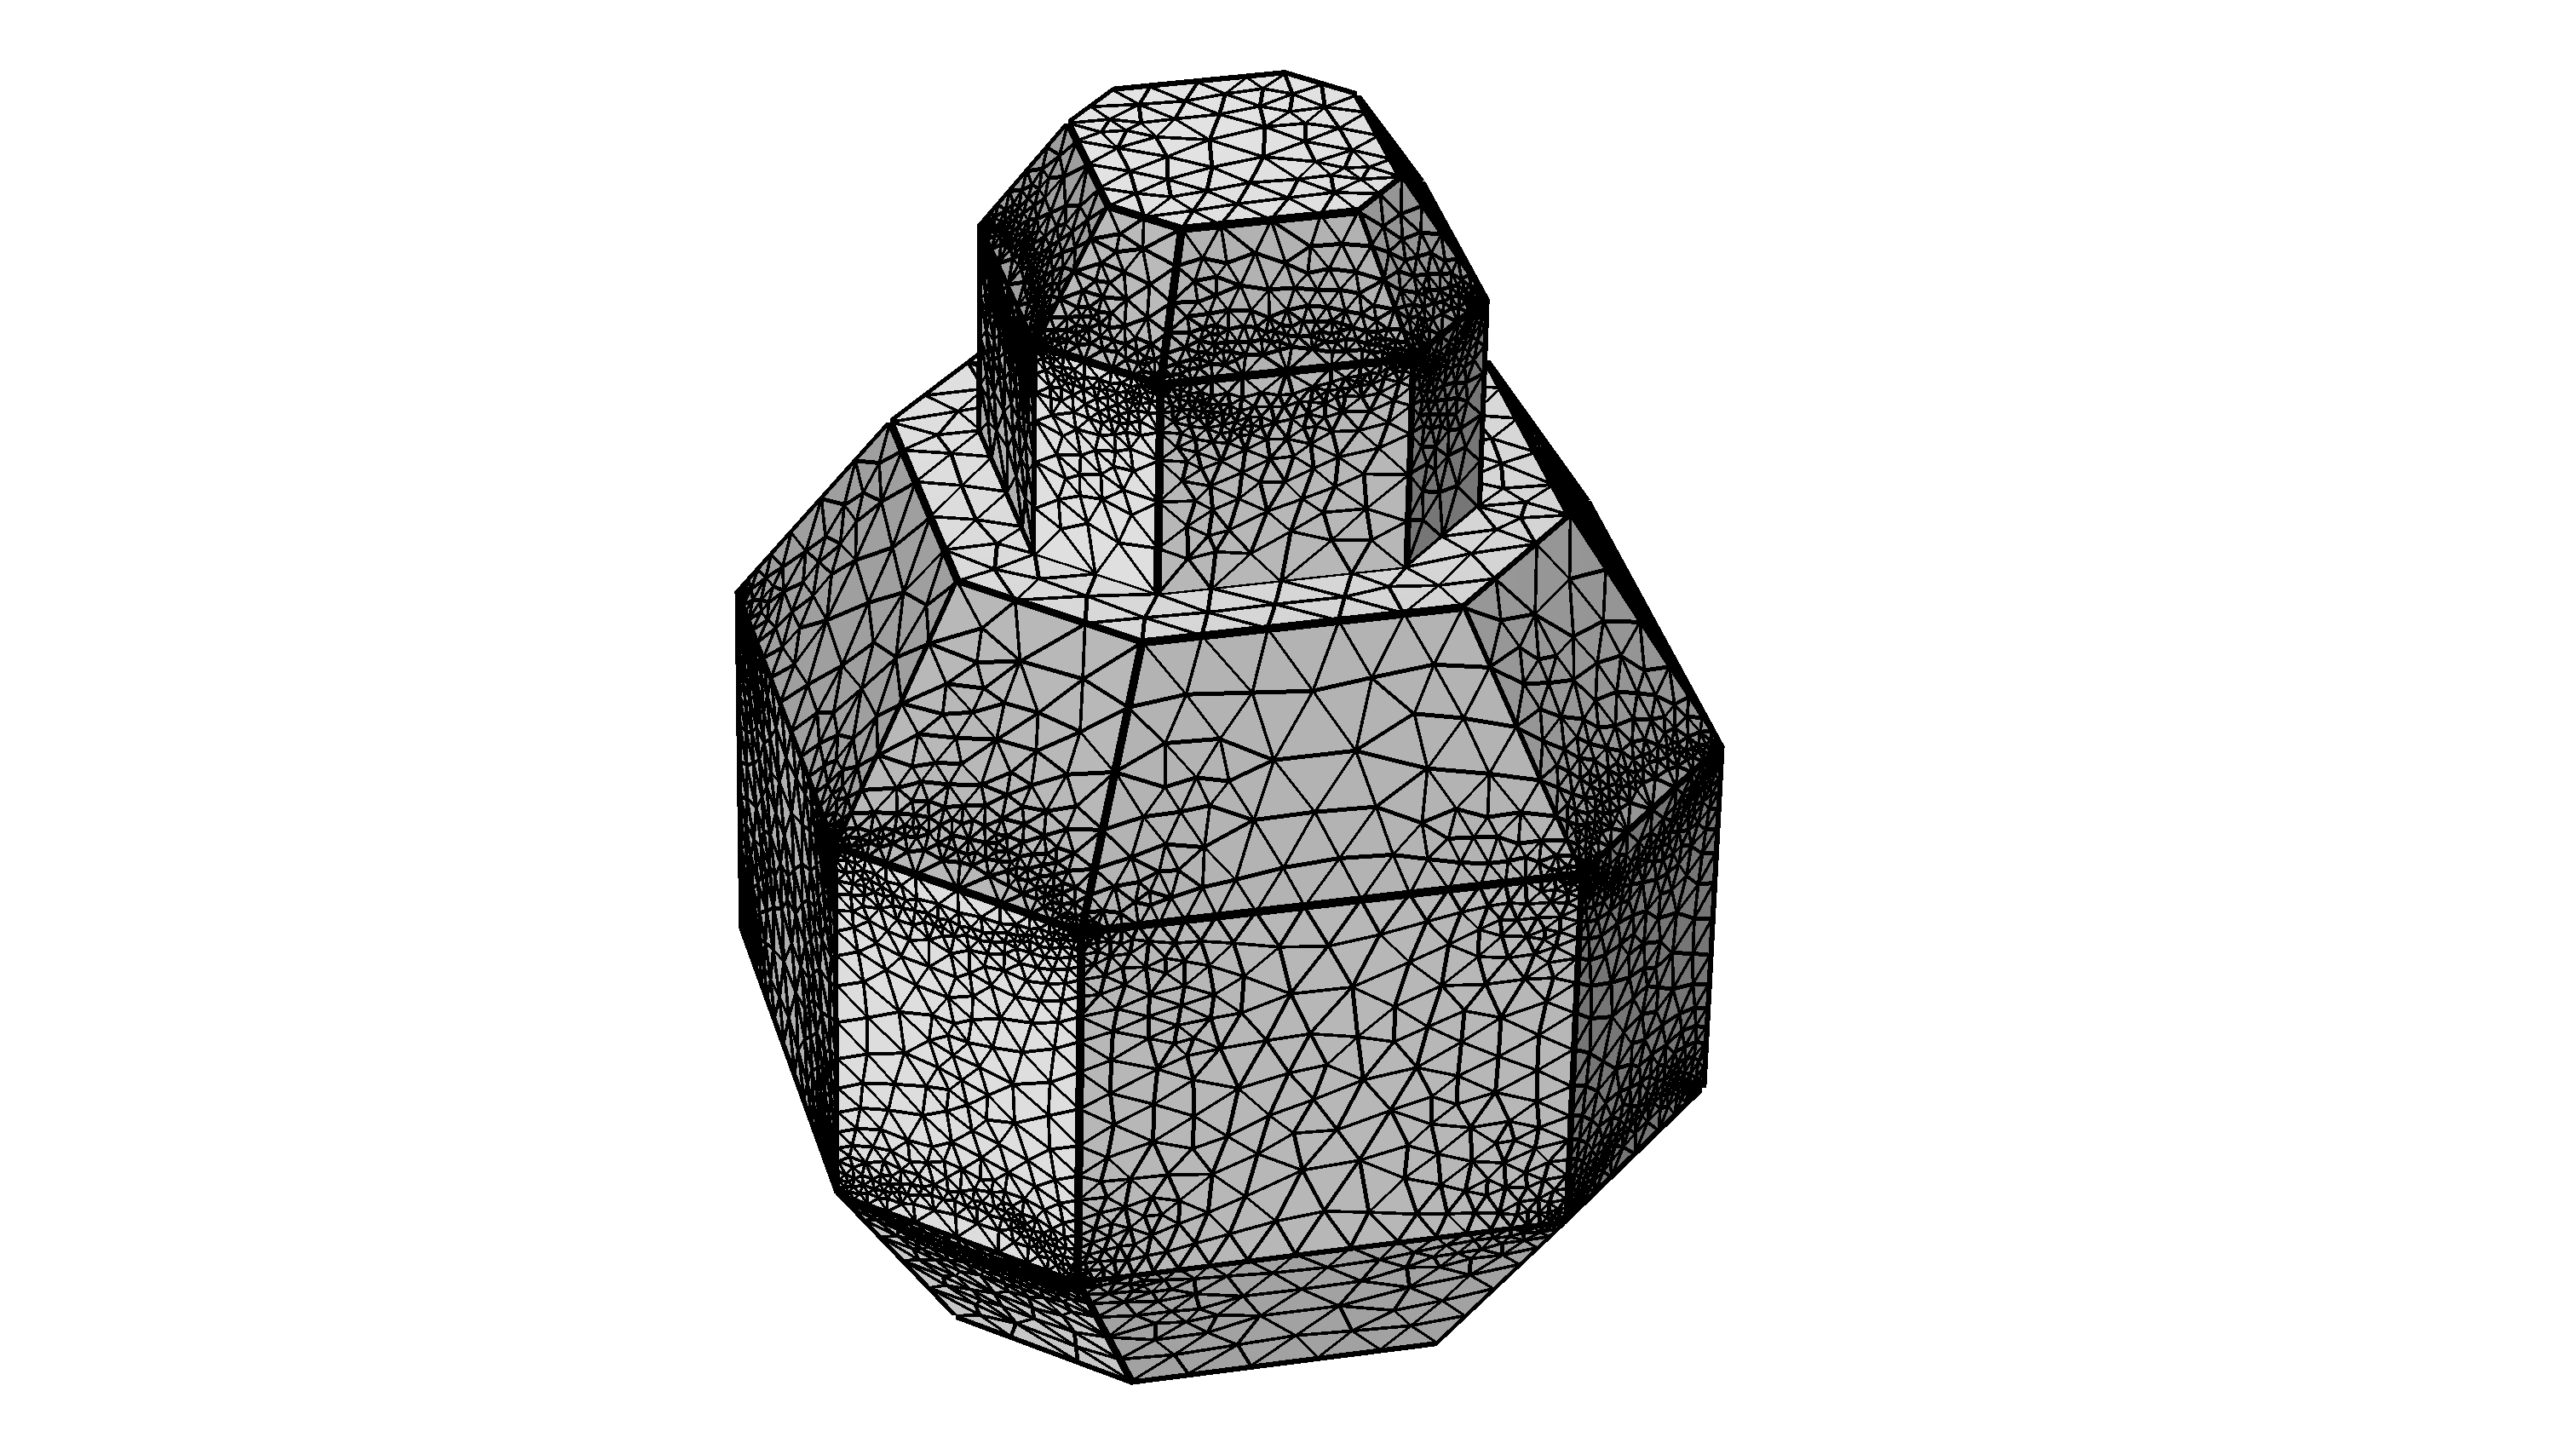
\includegraphics[width=0.5\textwidth]{INICTEL_Pictures/Mesh_SATBC.png}
        \caption{Mesh geometry for the SAT-BC configuration.}
        \label{fig:mesh_satbc}
    \end{figure}

    \item \textbf{SAT-B and SAT-C configuration:} This configuration represents the post-separation tethered state, where SAT-B and SAT-C are separated by the nominal maximum tether length of \(100~\mathrm{m}\). At this distance, SAT-B and SAT-C are evaluated as independent bodies for the EPS analysis, as shown in Figure~\ref{fig:mesh_separated}.

    \begin{figure}[H]
        \centering
        \begin{subfigure}[b]{0.54\textwidth}
            \centering
            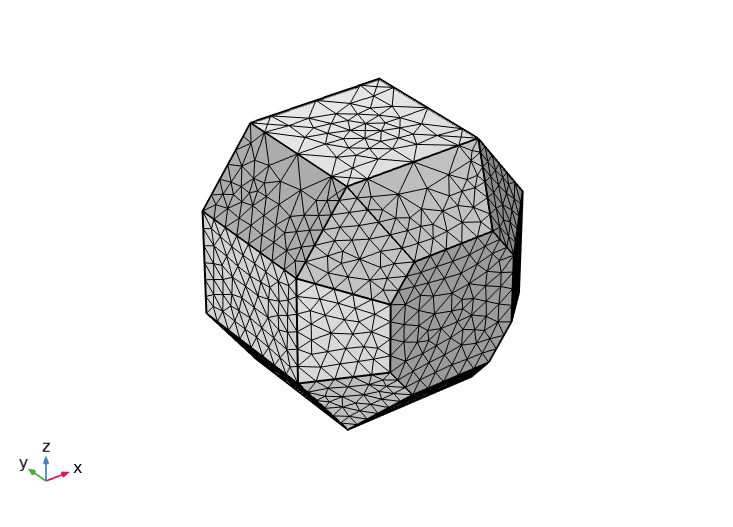
\includegraphics[width=\textwidth]{INICTEL_Pictures/Mesh_SATB.png}
            \caption{SAT-B mesh.}
        \end{subfigure}
        \begin{subfigure}[b]{0.45\textwidth}
            \centering
            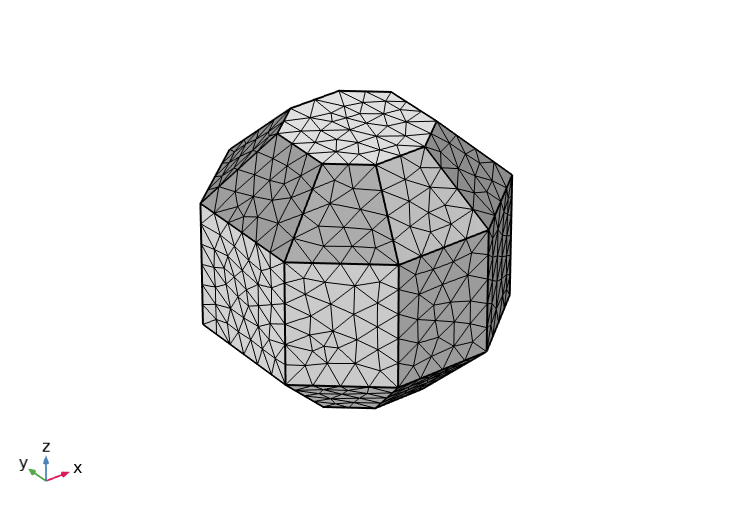
\includegraphics[width=\textwidth]{INICTEL_Pictures/Mesh_SATC.png}
            \caption{SAT-C mesh.}
        \end{subfigure}
        \caption{Independent mesh geometries for SAT-B and SAT-C at nominal maximum tether extension.}
        \label{fig:mesh_separated}
    \end{figure}
\end{itemize}

To improve computational efficiency and solver convergence during the thermodynamic simulations of the SAT-BC configuration, a simplified geometry of the SAT-BC assembly was implemented, as shown in Figure~\ref{fig:sat_bc_simplified}. The simplified geometry preserves the main external features needed for the EPS analysis, particularly the relative location of the solar-panel mounting areas and the possible self-shadowing between SAT-B and SAT-C.

Visual inspection of the detailed reference models was used to identify the polyhedral faces corresponding to the equatorial rings where the solar panels are physically mounted. This geometric information was then mapped onto the equivalent surfaces of the simplified SAT-BC mesh. In this way, the boundary conditions for solar absorptivity, \(\alpha\), and thermal emissivity, \(\epsilon\), were assigned to the appropriate surfaces. This procedure ensures that the simplified COMSOL model remains consistent with the intended solar-panel distribution while reducing the geometric complexity of the simulation.

\begin{figure}[h!]
    \centering
    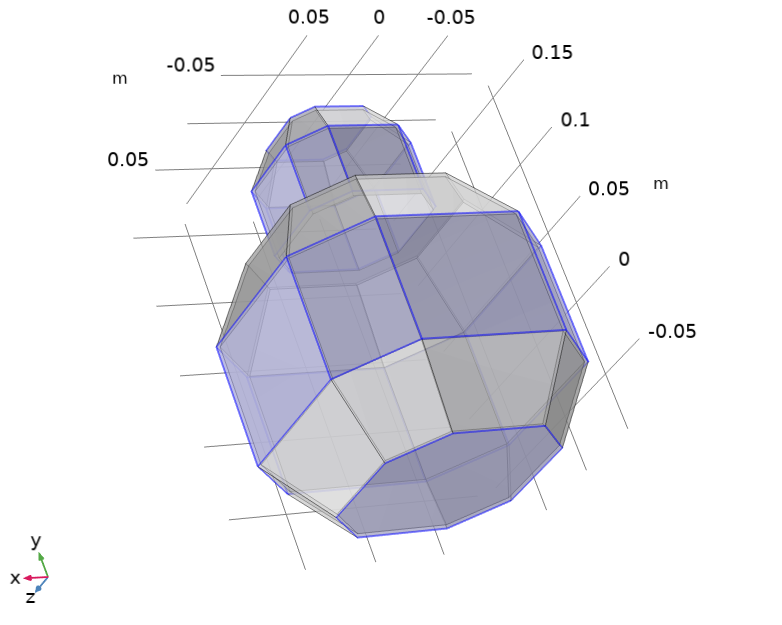
\includegraphics[width=0.75\textwidth]{INICTEL_Pictures/SatBCModelling.png}
    \caption{Simplified 3D model of the SAT-BC configuration used for COMSOL simulations.}
    \label{fig:sat_bc_simplified}
\end{figure}

\subsection{COMSOL Orbital Simulation Setup}
\label{sub:eps_comsol_simulation_setup}

The thermal-orbital simulations were implemented in COMSOL Multiphysics using a coupled approach between the \textit{Orbital Thermal Loads} (\texttt{otl}) and \textit{Heat Transfer in Solids} (\texttt{ht}) interfaces. The \textit{Orbital Thermal Loads} interface was used to calculate the external radiative heat fluxes acting on the satellite surfaces, while the \textit{Heat Transfer in Solids} interface was used to estimate the resulting conductive heat distribution within the satellite structures. This coupled setup allows the external orbital radiative loads and the internal conductive thermal response of the satellite structures to be evaluated within the same simulation framework.

\subsubsection{Orbital Thermal Loads}
\label{subsub:eps_orbital_thermal_loads}

The \textit{Orbital Thermal Loads} interface defines the orbital environment and the radiative exchange between the spacecraft, the Sun, and the planet. Two inclination cases were simulated: a \(30^\circ\) prograde orbit and a \(94^\circ\) near-polar orbit. These cases were selected to compare different illumination and eclipse conditions affecting the solar power-generation capability of the satellite configurations. Table~\ref{tab:orbital_params} summarizes the fixed and variable orbital parameters used in the simulations.

\begin{table}[h!]
\centering
\caption{Orbital parameters used for the EPS simulations.}
\label{tab:orbital_params}
\renewcommand{\arraystretch}{1.5}
\begin{tabular}{|l|c|l|}
\hline
\textbf{Parameter} & \textbf{Value} & \textbf{Description} \\ \hline
Orbit type & Circular & General geometry of the orbit \\ \hline
Semimajor axis, \(a\) & \(R_{\mathrm{planet}} + 700~\mathrm{km}\) & Radius from the planetary center \\ \hline
Eccentricity, \(e\) & \(0\) & Circular orbit condition \\ \hline
Inclination, \(i\) & \(30^\circ / 94^\circ\) & Prograde and near-polar cases \\ \hline
Right ascension of the ascending node, \(\Omega\) & \(0^\circ\) & Orientation of the orbital plane \\ \hline
Argument of periapsis, \(\omega\) & \(0^\circ\) & Reference orientation within the orbital plane \\ \hline
Initial true anomaly, \(\nu_0\) & \(0^\circ\) & Initial spacecraft position at \(t=0\) \\ \hline
\end{tabular}
\end{table}

The main model features used in the orbital thermal setup are summarized as follows:

\begin{itemize}
    \item \textbf{Sun and Planet Properties:} These features define the external radiative environment. The Sun properties define the direct solar input, including the solar constant, \(G_{sc}\), while the planet properties define the planetary radius, albedo, and infrared (IR) emission.

    \item \textbf{Orbital Parameters:} This feature defines the spacecraft trajectory using the orbital elements listed in Table~\ref{tab:orbital_params}. The semimajor axis is set as \(R_{\mathrm{planet}} + 700~\mathrm{km}\), with \(e=0\), corresponding to a circular LEO case.

    \item \textbf{Spacecraft Axes and Orientation:} This feature defines the local spacecraft coordinate system and the nadir-pointing attitude condition used in the EPS analysis. The main longitudinal axis of each satellite configuration is aligned with the local nadir direction in the LVLH frame.

    \item \textbf{Generate Events Interface:} This feature identifies discrete orbital events, including entry into and exit from planetary eclipse.
\end{itemize}

\subsubsection{Surface and Material Properties}
\label{subsub:eps_surface_material_properties}

The interaction between the satellite geometry and the orbital radiative environment is defined through the surface radiation properties assigned to the external faces:

\begin{itemize}
    \item \textbf{Diffuse Surface:} This feature assigns the thermo-optical properties of the external surfaces, including solar absorptivity, \(\alpha\), and thermal emissivity, \(\epsilon\). These parameters determine how much incident radiation is absorbed and how much thermal radiation is emitted back to space.

    \item \textbf{Opacity:} This setting defines which surfaces are opaque to radiation. It is required to account for self-shadowing effects, particularly in the SAT-BC configuration.
\end{itemize}

\subsubsection{Heat Transfer in Solids}
\label{subsub:eps_heat_transfer_solids}
The \textit{Heat Transfer in Solids} interface estimates the temperature distribution within the satellite structures resulting from the external radiative loads. This interface accounts for conductive heat transfer through the spacecraft shell and internal structural elements. The initial temperature is defined through the \textit{Initial Values} feature at \(t=0\).


\subsection{Power Generation Results and Operational Constraints}
\label{sub:eps_power_generation_results}
For the SAT-ABC configuration, the EPS analysis considers the external solar-array surfaces of the SAT-A bus as the active power-generation surfaces. Figure~\ref{fig:satabc_irradiation} shows the resulting surface irradiation profiles for the \(30^\circ\) and \(94^\circ\) inclination cases. The \(30^\circ\) case reaches peak incident values close to \(115~\mathrm{W}\), but includes a pronounced eclipse interval in which the incident power drops to zero. In contrast, the \(94^\circ\) case provides a higher and more continuous irradiation profile, with peak incident values close to \(132~\mathrm{W}\) and no deep eclipse interval in the simulated orbit. These results provide the reference power-generation capability of the satellite system before the deployment of SAT-BC.

\begin{figure}[h!]
    \centering
    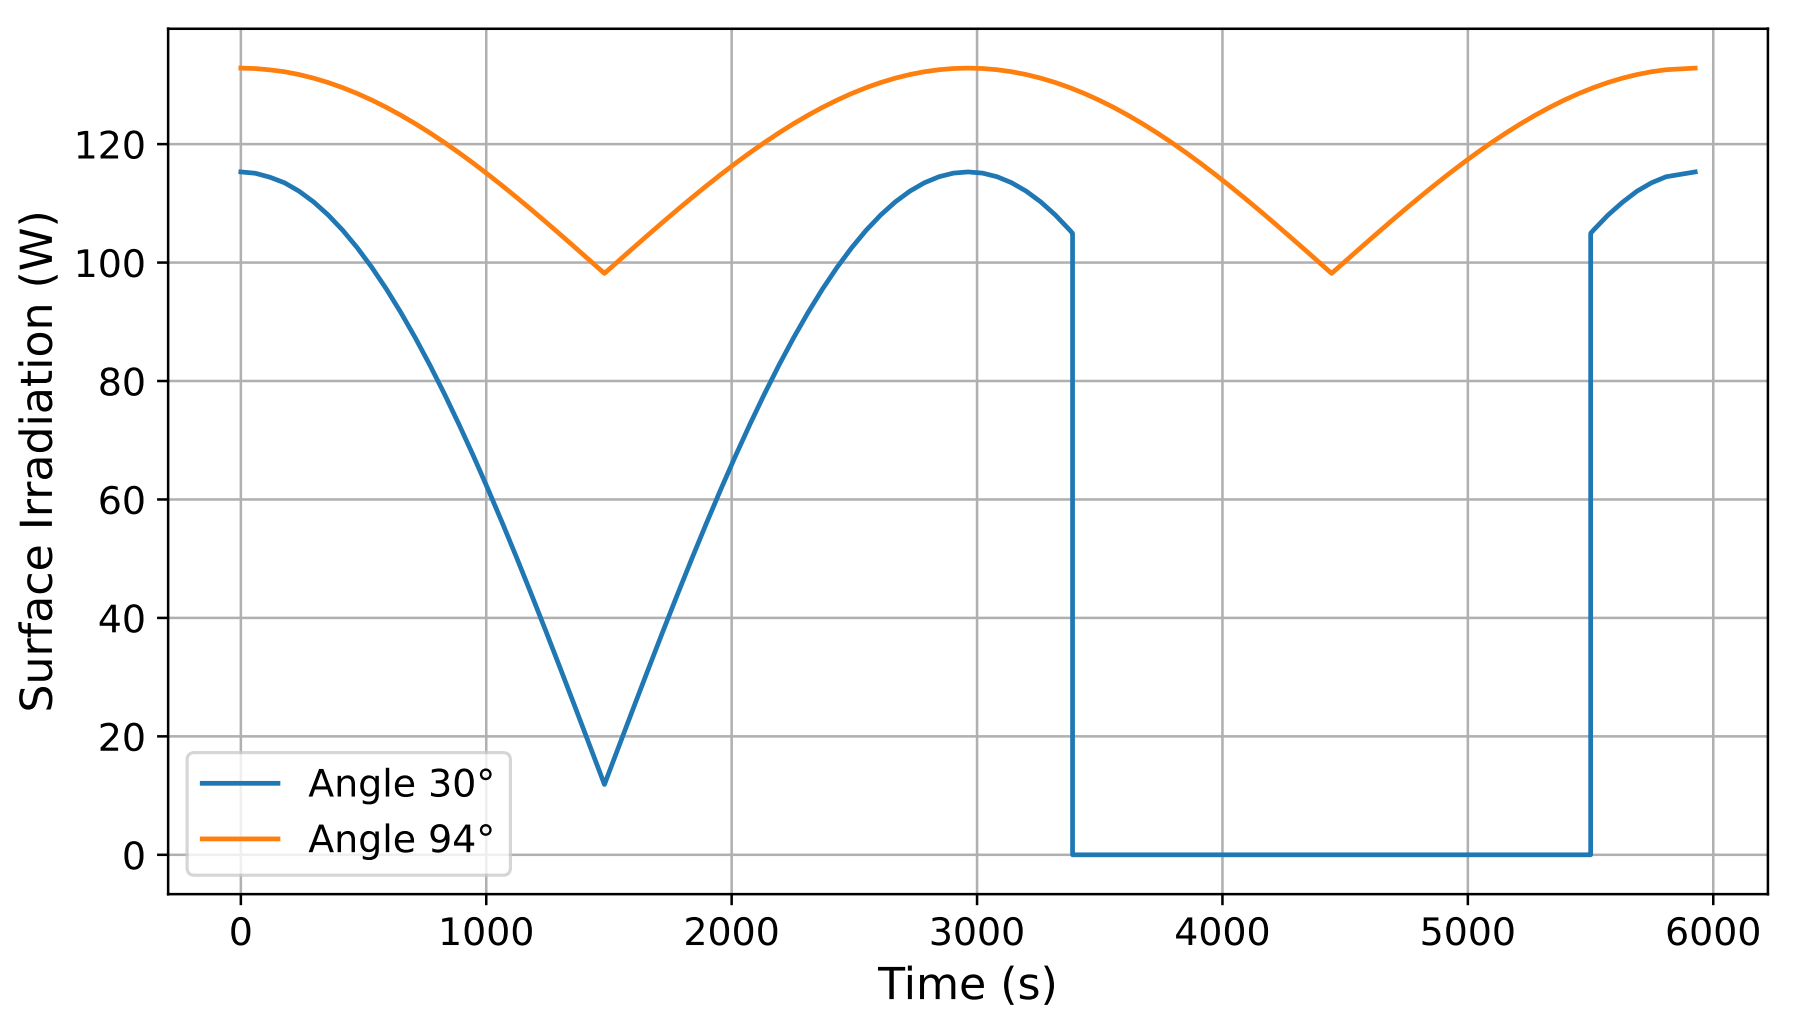
\includegraphics[height=6cm, keepaspectratio]{INICTEL_Pictures/Phase1_SATA_irradiation.png}
    \caption{Surface irradiation profile for the SAT-ABC configuration.}
    \label{fig:satabc_irradiation}
\end{figure}

Figure~\ref{fig:satbc_irradiation} shows the total incident surface irradiation for the SAT-BC configuration under the \(30^\circ\) and \(94^\circ\) inclination cases. In this configuration, the combined geometry affects the illuminated area and introduces possible self-shadowing between SAT-B and SAT-C. The \(30^\circ\) case reaches a higher peak incident power of approximately \(29.5~\mathrm{W}\), but includes an eclipse interval in which the incident solar power drops to zero. In contrast, the \(94^\circ\) case provides a lower but more continuous irradiation profile, with peak incident values of approximately \(14.5~\mathrm{W}\). This comparison indicates that the SAT-BC configuration is sensitive to both orbital illumination conditions and self-shadowing effects.

\begin{figure}[h!]
    \centering
    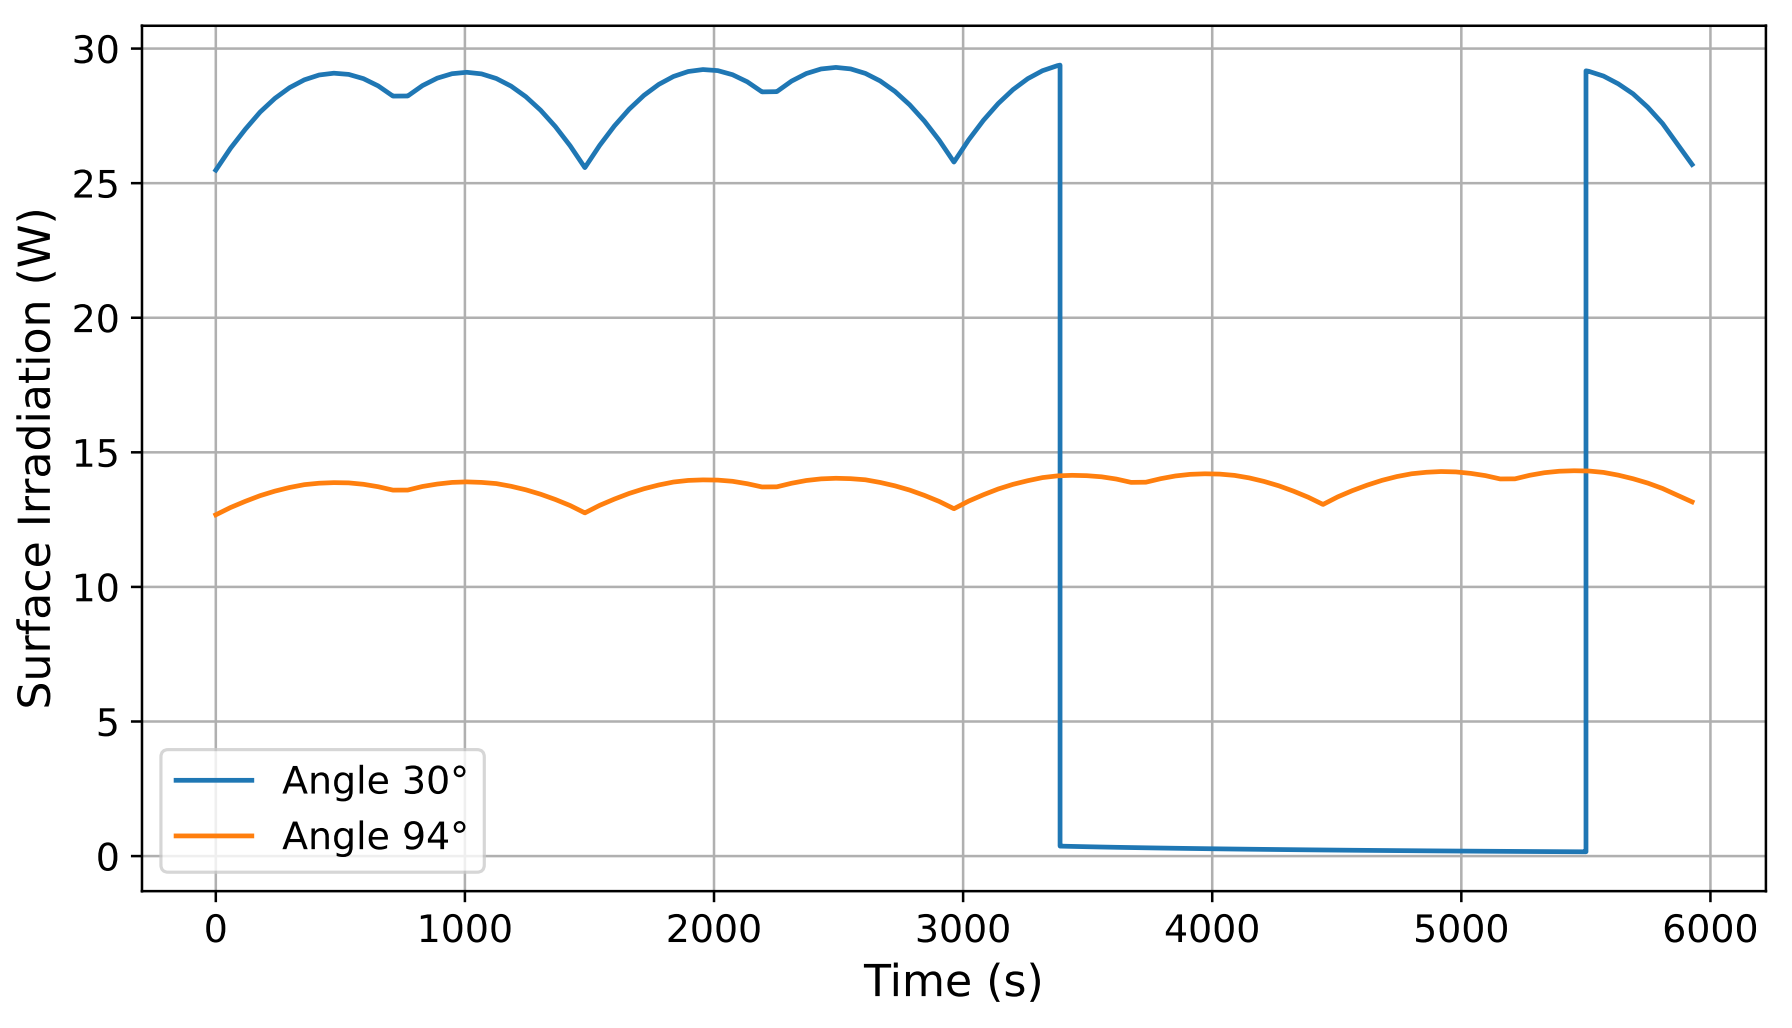
\includegraphics[height=6cm, keepaspectratio]{INICTEL_Pictures/Phase2_SATBC_irradiation.png}
    \caption{Total surface irradiation profile for the SAT-BC configuration.}
    \label{fig:satbc_irradiation}
\end{figure}

Figure~\ref{fig:satb_satc_irradiation} compares the incident surface irradiation profiles for SAT-B, SAT-C, and the combined SAT-B and SAT-C system at the nominal maximum tether extension of \(100~\mathrm{m}\). At this separation distance, mutual self-shadowing between the satellites is neglected in the EPS analysis. SAT-B reaches peak incident values close to \(40~\mathrm{W}\), while SAT-C reaches lower peak values close to \(12.8~\mathrm{W}\), consistent with its smaller active surface area. The \(30^\circ\) case presents distinct sunlit and eclipse intervals, whereas the \(94^\circ\) case provides a more continuous illumination profile.

\begin{figure}[H]
    \centering
    \subfloat[SAT-B irradiation]{
        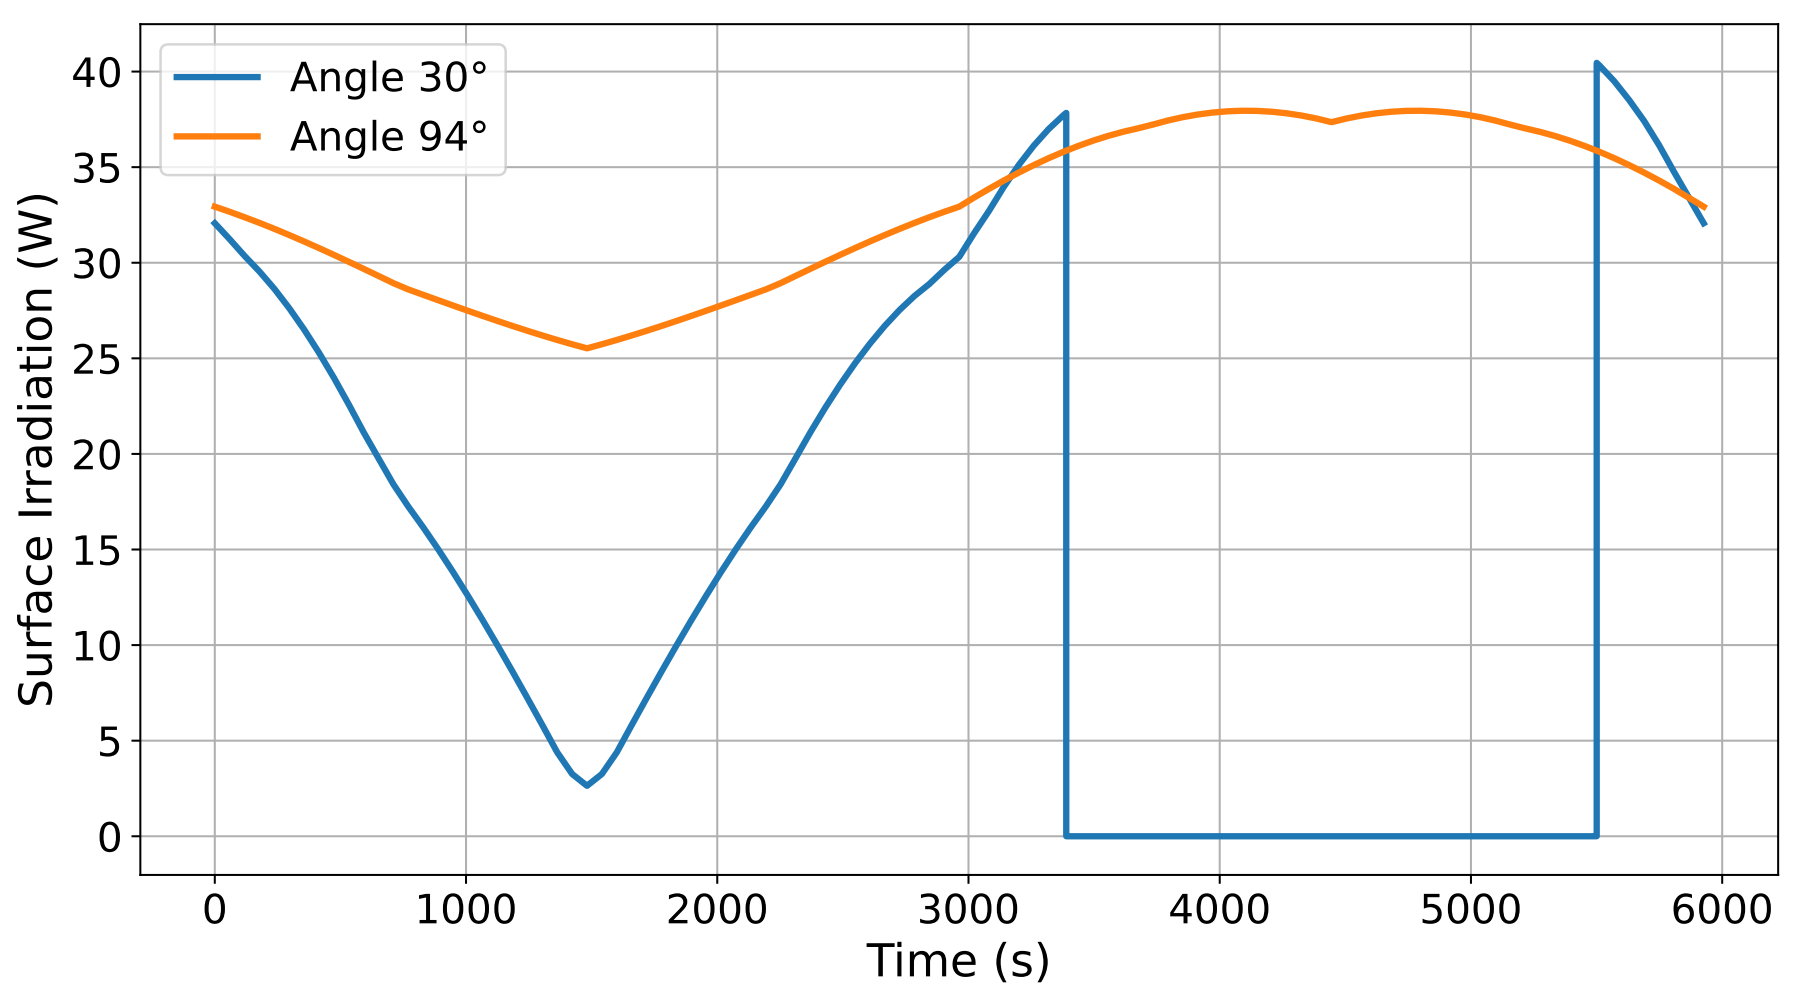
\includegraphics[height=6cm, keepaspectratio
        ]{INICTEL_Pictures/Phase3_SATB_irradiation.png}
        \label{fig:satb_irradiation}
    }\\[0.3em]
    \subfloat[SAT-C irradiation]{
        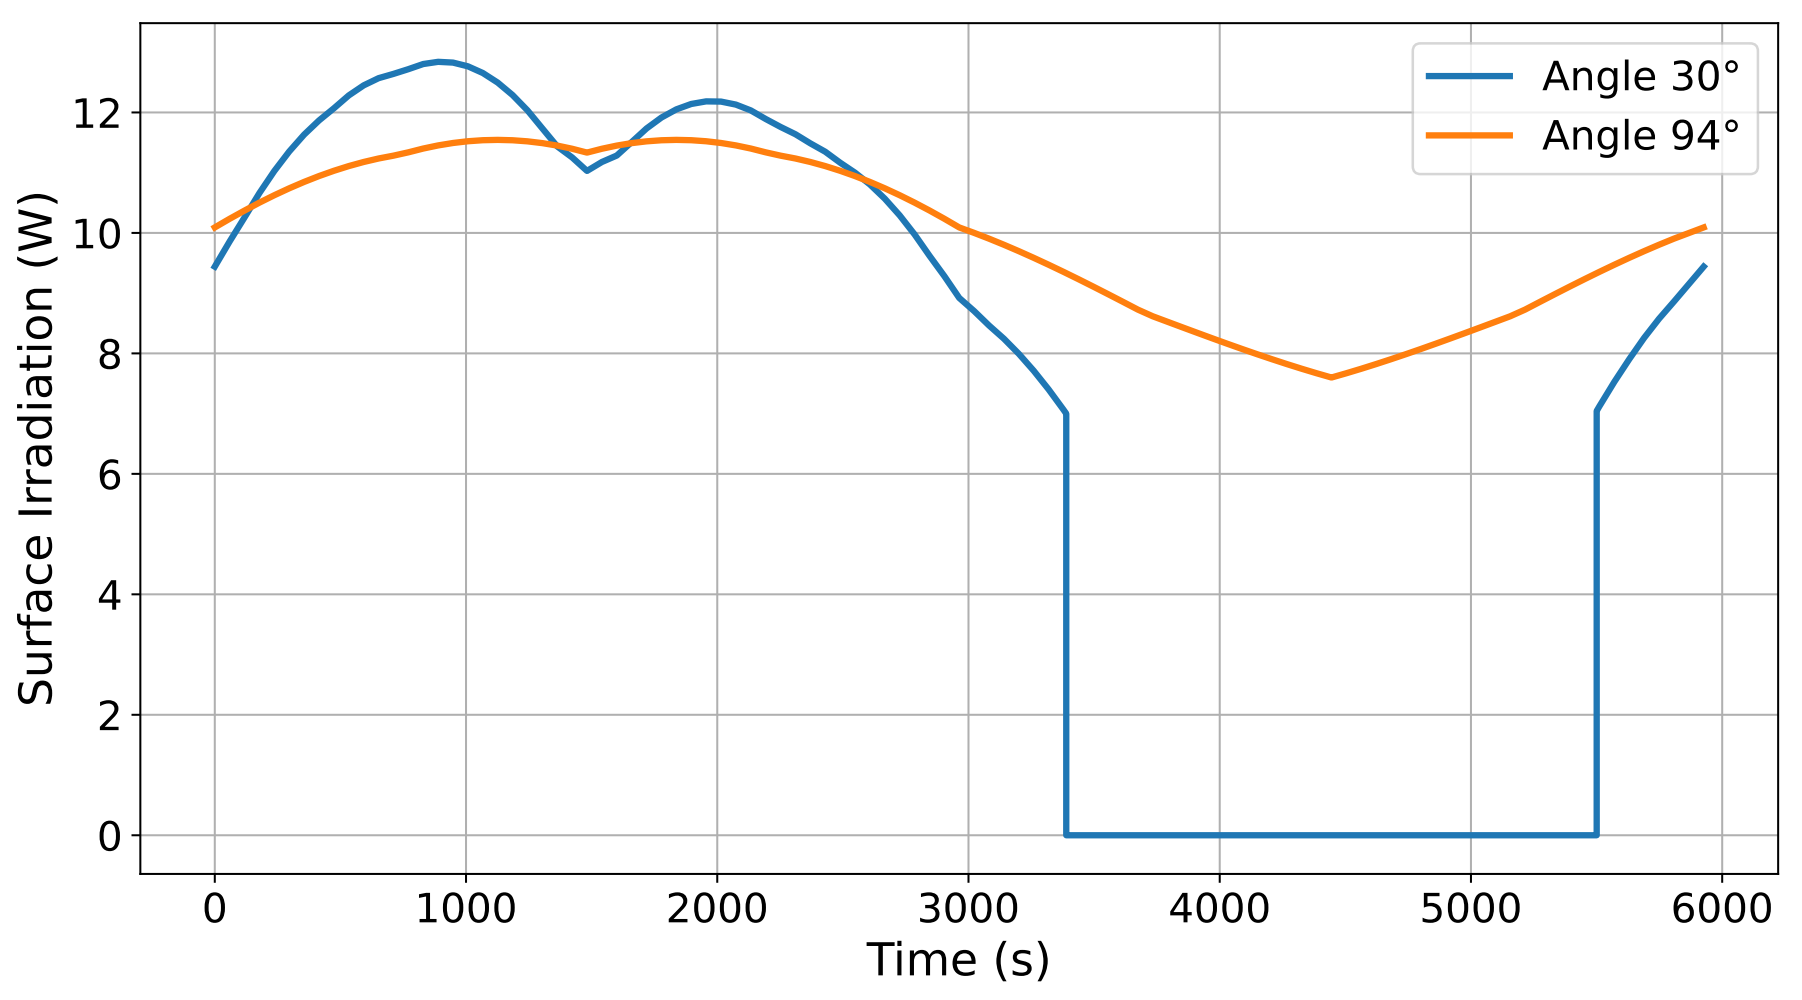
\includegraphics[height=6cm, keepaspectratio
        ]{INICTEL_Pictures/Phase3_SATC_irradiation.png}
        \label{fig:satc_irradiation}
    }\\[0.3em]
    \subfloat[Total SAT-B and SAT-C irradiation]{
        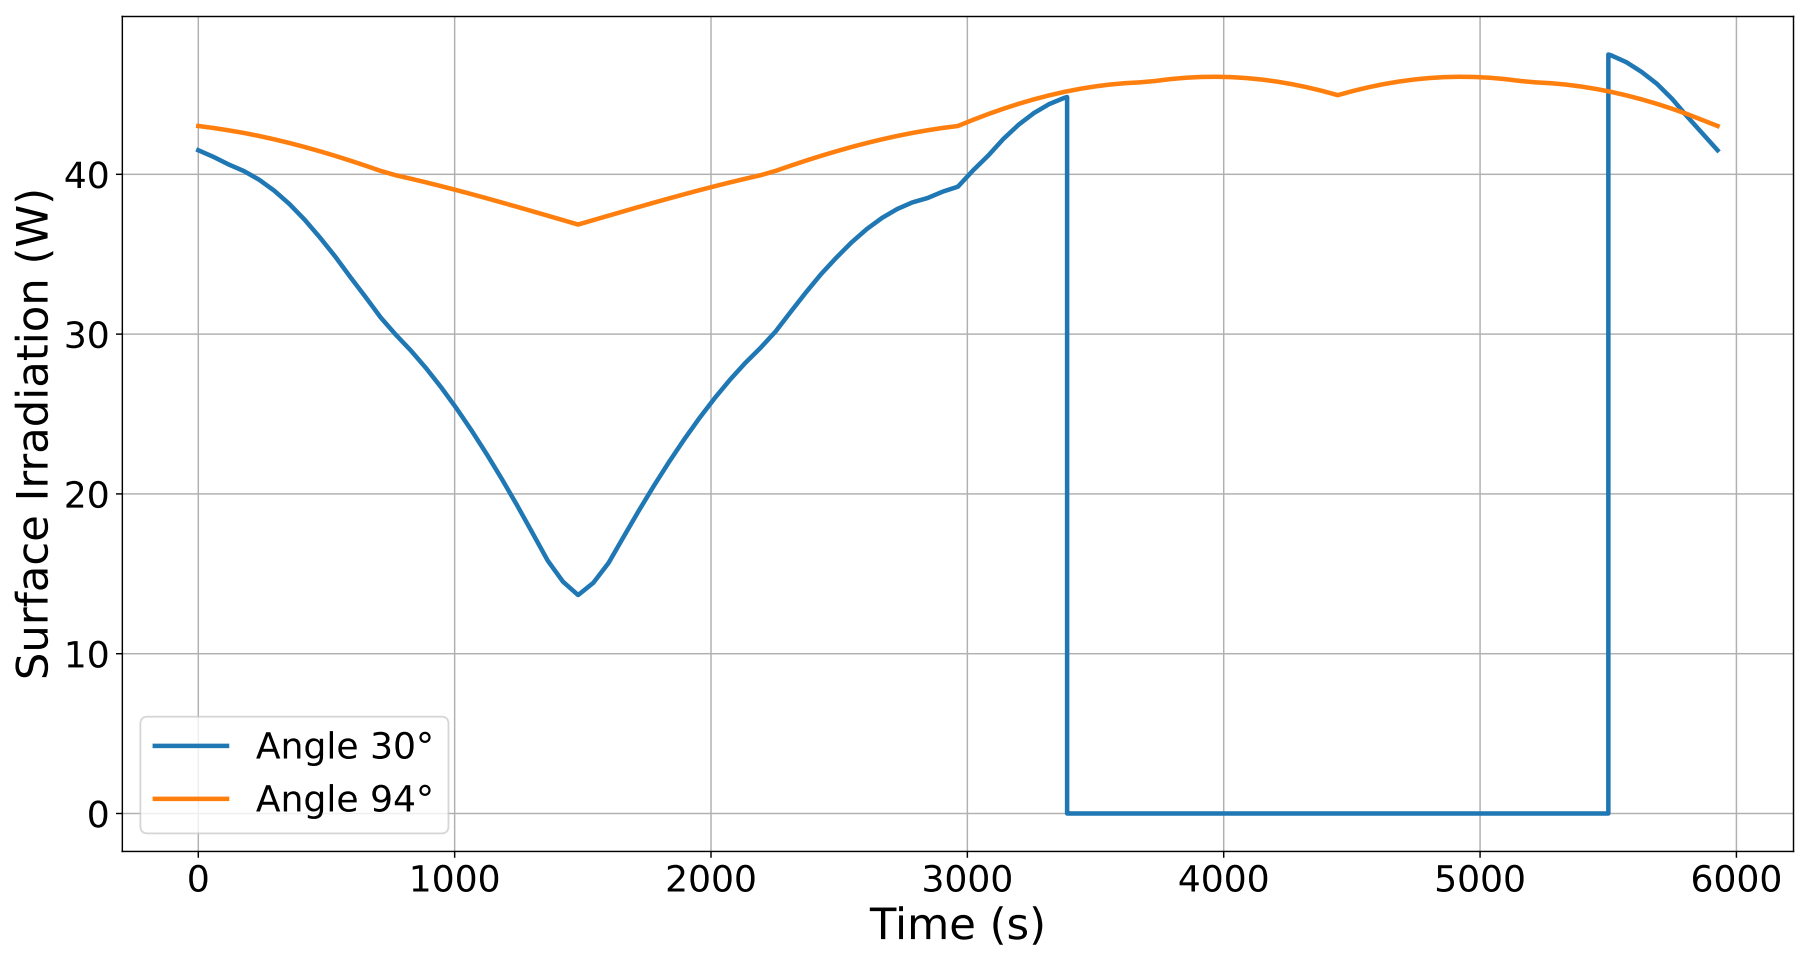
\includegraphics[height=6cm, keepaspectratio
        ]{INICTEL_Pictures/Phase3_All_irradiation.png}
        \label{fig:satb_satc_total_irradiation}
    }
    \caption{Surface irradiation profiles for SAT-B, SAT-C, and the combined SAT-B and SAT-C system at nominal maximum tether extension.}
    \label{fig:satb_satc_irradiation}
\end{figure}

The temperature profiles obtained from the thermal simulation were used to adjust the system-level efficiency factor, \(\eta_{\mathrm{sys}}\), allowing the preliminary power estimate to account for temperature-dependent solar-cell performance during sunlit and eclipse portions of the orbit. Therefore, the results must be interpreted not only in terms of peak incident power, but also considering eclipse intervals, thermal effects, and the different power-generation capability of each satellite configuration.

\subsubsection{Peak Power Generation Summary}
\label{subsub:eps_peak_power_generation_summary}

Based on the conversion methodology defined in Eq.~\eqref{eq:eps_electrical_power_conversion}, using \(\eta_{\mathrm{cell}} \approx 0.30\), \(P_F = 0.80\), and \(\eta_{\mathrm{sys}} \approx 0.85\), the net conversion efficiency from incident solar power to usable electrical power is approximately \(20\%\). The peak irradiation values extracted from the orbital simulations are therefore converted into estimated peak electrical power values for each configuration.

Table~\ref{tab:power_generation} summarizes the peak incident surface irradiation, \(P_{\mathrm{in}}\), and the corresponding estimated peak electrical power, \(P_{\mathrm{elec}}\), for the \(30^\circ\) and \(94^\circ\) inclination cases. The last column indicates whether the simulated profile includes an eclipse interval, defined here as an interval in which \(P_{\mathrm{in}}\) drops to zero.

\begin{table}[h!]
\centering
\caption{Summary of peak surface irradiation and estimated usable electrical power for the EPS simulation cases, assuming \(\eta_{\mathrm{total}} \approx 20\%\).}
\label{tab:power_generation}
\renewcommand{\arraystretch}{1.3}
\resizebox{\textwidth}{!}{%
\begin{tabular}{|l|c|c|c|c|}
\hline
\textbf{Configuration} & \textbf{Inclination} & \textbf{Peak Incident \(P_{\mathrm{in}}\)} & \textbf{Est. Peak Electrical \(P_{\mathrm{elec}}\)} & \textbf{Eclipse Condition} \\ \hline
SAT-ABC & \(30^\circ\) & \(\sim 115.0~\mathrm{W}\) & \(\sim 23.0~\mathrm{W}\) & Eclipse, \(P_{\mathrm{in}} \rightarrow 0\) \\ \hline
SAT-ABC & \(94^\circ\) & \(\sim 132.0~\mathrm{W}\) & \(\sim 26.4~\mathrm{W}\) & No eclipse interval, \(P_{\mathrm{in}} > 0\) \\ \hline
SAT-BC & \(30^\circ\) & \(\sim 29.5~\mathrm{W}\) & \(\sim 5.9~\mathrm{W}\) & Eclipse, \(P_{\mathrm{in}} \rightarrow 0\) \\ \hline
SAT-BC & \(94^\circ\) & \(\sim 14.5~\mathrm{W}\) & \(\sim 2.9~\mathrm{W}\) & No eclipse interval, \(P_{\mathrm{in}} > 0\) \\ \hline
SAT-B & \(30^\circ\) & \(\sim 40.0~\mathrm{W}\) & \(\sim 8.0~\mathrm{W}\) & Eclipse, \(P_{\mathrm{in}} \rightarrow 0\) \\ \hline
SAT-B & \(94^\circ\) & \(\sim 38.0~\mathrm{W}\) & \(\sim 7.6~\mathrm{W}\) & No eclipse interval, \(P_{\mathrm{in}} > 0\) \\ \hline
SAT-C & \(30^\circ\) & \(\sim 12.8~\mathrm{W}\) & \(\sim 2.6~\mathrm{W}\) & Eclipse, \(P_{\mathrm{in}} \rightarrow 0\) \\ \hline
SAT-C & \(94^\circ\) & \(\sim 11.5~\mathrm{W}\) & \(\sim 2.3~\mathrm{W}\) & No eclipse interval, \(P_{\mathrm{in}} > 0\) \\ \hline
\end{tabular}%
}
\end{table}

\subsubsection{Orbit-Average Power and Operational Constraints}
\label{subsub:eps_oap_operational_constraints}

Although Table~\ref{tab:power_generation} provides useful peak-power estimates, it does not constitute a complete electrical power budget. Detailed subsystem loads, battery sizing, duty cycles, and eclipse-energy balance must be refined in later design stages. Therefore, the final EPS design should be based on orbit-average power and energy balance.

The orbit-average generated power, \(OAP_{\mathrm{gen}}\), should be obtained by integrating the instantaneous generated electrical power over the orbital period, \(T_{\mathrm{orbit}}\), and comparing it with the average subsystem load, \(OAP_{\mathrm{load}}\). This comparison is required to assess whether the available generated power and stored energy are sufficient during both sunlit and eclipse portions of the orbit.

The preliminary results indicate different power-generation constraints for the considered configurations:

\begin{itemize}
    \item \textbf{SAT-ABC:} The SAT-ABC configuration benefits from the larger external surface area of the SAT-A bus. As a result, it provides the highest peak electrical power among the analyzed configurations and serves as the reference case before the deployment of SAT-BC.

    \item \textbf{SAT-BC:} The SAT-BC configuration presents the most constrained generation condition. The available illuminated area is reduced compared with SAT-ABC, and self-shadowing between SAT-B and SAT-C further limits the incident irradiation. The estimated peak electrical power ranges from approximately \(2.9~\mathrm{W}\) to \(5.9~\mathrm{W}\), indicating that this configuration may require low-power operation and conservative duty cycling until SAT-B/SAT-C separation.

    \item \textbf{SAT-B and SAT-C:} After SAT-B/SAT-C separation and deployment to nominal maximum tether extension, the two satellites are evaluated independently. SAT-B provides a higher estimated peak electrical power than SAT-C because of its larger active surface area. SAT-C remains the more constrained unit, with estimated peak electrical power between approximately \(2.3~\mathrm{W}\) and \(2.6~\mathrm{W}\), which suggests that its subsystem operation will require careful duty-cycle management.
\end{itemize}

A minimum power margin, \(PM\), should be defined in later EPS design stages to account for degradation, modeling uncertainty, conversion losses, and variations in operational load. If the available margin becomes insufficient under worst-case illumination or eclipse conditions, payload duty cycles and non-critical subsystem operation may need to be reduced to preserve essential spacecraft functions.


\subsection{Communications System}
\label{sub:communications_system}
The communications system supports satellite operation and tether-experiment data return. The architecture uses separate links for low-rate operational traffic and higher-volume mission-data downlink.

After SAT-BC is released from SAT-A, SAT-B becomes the communications node for the tether experiment. SAT-B receives data from SAT-C through a bidirectional inter-satellite link, combines those data with its own measurements, stores the resulting data products, and transmits selected information to the ground station. No direct communications link is considered between SAT-A and SAT-B or SAT-C after SAT-BC release. SAT-A retains an independent communications system for its own post-deployment operation. Table~\ref{tab:communications_links} summarizes the link parameters used in the current system architecture.

\begin{table}[htbp]
\centering
\caption{Communications links and reference sizing values for the LINKU mission.}
\label{tab:communications_links}
\small
\resizebox{\linewidth}{!}{%
\begin{tabular}{p{3.0cm}p{1.8cm}p{3.0cm}p{2.5cm}p{2.5cm}p{4.4cm}}
\toprule
\textbf{Link} &
\textbf{Direction} &
\textbf{Band / frequency} &
\textbf{Reference data rate} &
\textbf{Reference RF power} &
\textbf{Main function} \\
\midrule
SAT-B--Ground &
RX/TX &
UHF, \(437.2~\mathrm{MHz}\) &
\(9.6~\mathrm{kbps}\) &
\(1~\mathrm{W}\) TX &
TT\&C, housekeeping, and low-rate telemetry. \\

SAT-B--Ground &
TX only &
S-band, \(2.245~\mathrm{GHz}\) &
\(200~\mathrm{kbps}\) &
\(2~\mathrm{W}\) TX &
Selected tether-experiment data downlink. \\

SAT-B/SAT-C &
RX/TX &
Candidate \(2.4~\mathrm{GHz}\) short-range link &
\(1~\mathrm{Mbps}\) &
\(20~\mathrm{dBm}\) TX &
Experiment-data transfer and coordination. \\

SAT-A--Ground &
RX/TX &
UHF, \(437.2~\mathrm{MHz}\) &
\(9.6~\mathrm{kbps}\) &
\(1~\mathrm{W}\) TX &
SAT-A TT\&C, housekeeping, and low-rate telemetry. \\

SAT-A--Ground &
TX only &
S-band, \(2.245~\mathrm{GHz}\) &
\(200~\mathrm{kbps}\) &
\(2~\mathrm{W}\) TX &
SAT-A mission-data downlink. \\
\bottomrule
\end{tabular}%
}
\end{table}

The data-flow relation among the tether-experiment nodes is shown in Figure~\ref{fig:communications_data_flow}.

\begin{figure}[htbp]
    \centering
    \includegraphics[
        width=0.95\linewidth,
        height=9cm,
        keepaspectratio
    ]{PUCP_pictures/linku_tether_comms_v3}
    \caption{Communications and data-flow architecture for the LINKU tether experiment.}
    \label{fig:communications_data_flow}
\end{figure}

The SAT-B/SAT-C link is bidirectional because experiment data and control functions are distributed between the two satellites. The main data flow is from SAT-C to SAT-B before downlink, while the reverse direction supports command, acquisition control, timing coordination, acknowledgments, and retransmission requests. A short-range link around \(2.4~\mathrm{GHz}\) is retained as the main candidate because the nominal separation between SAT-B and SAT-C is limited by the \(100~\mathrm{m}\) tether length and compact communication modules are available in this frequency range.

All antennas mounted on SAT-B and SAT-C must be compact and non-deployable. This constraint is driven by the tethered configuration: deployable antennas or protruding mechanisms could introduce mechanical interference, increase the risk of tether contact, or create additional entanglement hazards during and after deployment. The antenna selection must therefore balance link margin, angular coverage, polarization robustness, and mechanical integration within the non-standard SAT-B and SAT-C geometries.

The data budget is expected to be dominated by the camera system. The current observation architecture uses three \(12~\mathrm{MP}\) cameras: two cameras installed on SAT-B and one camera installed on SAT-C. GNSS measurements, tether-tension measurements, inertial data, and housekeeping telemetry require significantly lower data rates. Therefore, the communications system is not sized for continuous downlink of raw full-resolution images. Instead, image acquisition is combined with onboard storage, image prefiltering, compression, and selective downlink.

During the SAT-B/SAT-C separation and tether-deployment interval, the image-acquisition rate may be higher than during the later stable tethered-system observation period. Saturated, overexposed, or non-informative images should be discarded before downlink. The remaining images are compressed and prioritized together with the corresponding GNSS, tension, inertial, and housekeeping data. This approach reduces the required downlink volume and allows the S-band link to be used more efficiently during available ground-station passes.

For sizing purposes, the S-band downlink rate is set to \(200~\mathrm{kbps}\). A \(10~\mathrm{min}\) ground-station pass at this rate provides a raw transmission capacity of approximately \(120~\mathrm{Mbit}\), equivalent to \(15~\mathrm{MB}\), before accounting for protocol overhead, coding, retransmissions, and link-margin constraints. This capacity is compatible with selected compressed experiment data, but not with continuous downlink of raw full-resolution images from all cameras.

Reference link-budget cases were defined to check the physical consistency of the selected communication links. The satellite-to-ground cases use the representative LEO altitude adopted in the EPS analysis, \(h=700~\mathrm{km}\). For a representative low-elevation pass, a minimum elevation of \(5^\circ\) is considered, giving a slant range of approximately \(2562~\mathrm{km}\). The SAT-B/SAT-C case uses the nominal maximum tether length of \(100~\mathrm{m}\). The free-space path loss is computed as

\begin{equation}
    L_\mathrm{FS} =
    32.44 + 20\log_{10}(f_\mathrm{MHz}) + 20\log_{10}(d_\mathrm{km}),
\end{equation}

where \(f_\mathrm{MHz}\) is the frequency in MHz and \(d_\mathrm{km}\) is the link distance in km. The received power is estimated as

\begin{equation}
    P_\mathrm{RX} =
    P_\mathrm{TX} + G_\mathrm{TX} + G_\mathrm{RX}
    - L_\mathrm{FS} - L_\mathrm{add},
\end{equation}

where \(P_\mathrm{TX}\) is the RF output power, \(G_\mathrm{TX}\) and \(G_\mathrm{RX}\) are the transmitter and receiver antenna gains, and \(L_\mathrm{add}\) represents additional implementation, polarization, and pointing losses. In the reference cases, \(L_\mathrm{add}=3~\mathrm{dB}\) is used.

\begin{table}[htbp]
\centering
\caption{Reference link-budget cases for the LINKU communications architecture.}
\label{tab:communications_link_budget_cases}
\small
\resizebox{\linewidth}{!}{%
\begin{tabular}{lccccccccc}
\toprule
\textbf{Case} &
\textbf{Frequency} &
\textbf{Range} &
\textbf{Data rate} &
\textbf{\(P_\mathrm{TX}\)} &
\textbf{\(G_\mathrm{TX}\)} &
\textbf{\(G_\mathrm{RX}\)} &
\textbf{\(L_\mathrm{FS}\)} &
\textbf{\(L_\mathrm{add}\)} &
\textbf{\(P_\mathrm{RX}\)} \\
&
\textbf{[MHz]} &
\textbf{[km]} &
\textbf{[bps]} &
\textbf{[dBm]} &
\textbf{[dBi]} &
\textbf{[dBi]} &
\textbf{[dB]} &
\textbf{[dB]} &
\textbf{[dBm]} \\
\midrule
SAT-B--Ground UHF &
437.2 &
2562 &
\(9.6\times10^{3}\) &
30 &
0 &
12 &
153.4 &
3 &
-114.4 \\

SAT-B--Ground S-band &
2245 &
2562 &
\(2.0\times10^{5}\) &
33 &
3 &
30 &
167.6 &
3 &
-104.6 \\

SAT-B/SAT-C \(2.4~\mathrm{GHz}\) &
2400 &
0.1 &
\(1.0\times10^{6}\) &
20 &
0 &
0 &
80.0 &
3 &
-63.0 \\
\bottomrule
\end{tabular}%
}
\end{table}

Using the transmitter powers in Table~\ref{tab:communications_link_budget_cases}, the received-power estimates support the selected data-rate assumptions with standard small-satellite transmitter powers and compact antenna gains. The SAT-B/SAT-C case provides a higher received-power level than the spacecraft-to-ground cases because its range is limited to the tether length.

At the next design stage, these estimates should be converted into closed link budgets using the selected modulation and coding scheme, receiver and system noise parameters, antenna patterns, loss terms, and ground-station configuration. In parallel, the data budget, image-compression and filtering approach, and SAT-B/SAT-C link implementation should be consolidated so that antenna integration, frequency-allocation constraints, and ground-station compatibility are assessed against a consistent communications configuration.


\begin{comment}
\section{Attitude Determination and Control System}

\subsection{Concept of operations}
The Attitude Determination and Control Subsystem (ADCS) for the Linku project is designed according to the mission phases presented in the other documents. The mission phases are defined as follows:

\begin{itemize}
    \item \textbf{Phase 1:} SAT-A is released from the deployer with a non-zero initial angular rate. At this stage, SAT-A contains SAT-B and SAT-C, acting as a single rigid body referred to as SAT-ABC. This leads to tumbling during the initial moments after deployment.
    \item \textbf{Phase 2:} Body SAT-ABC gradually reduces its rotation rate (detumbling) and subsequently achieves attitude stabilization using an ADCS composed of magnetorquers and reaction wheels.
    \item \textbf{Phase 3:} Body SAT-ABC enters a settling mode for approximately one hour to verify the performance of the attitude determination algorithm and allow for the necessary convergence time.
    \item \textbf{Phase 4:} Body SAT-ABC orients itself along the RAM direction (orbital velocity vector) to prepare for the deployment of SAT-B and SAT-C.
    \item \textbf{Phase 5:} SAT-A deploys the coupled satellite system consisting of SAT-B and SAT-C.
\end{itemize}

Up to this stage, the system is modeled as a single rigid body (SAT-A containing SAT-B and SAT-C). In the subsequent phases, the mission will consider two distinct entities: SAT-A (post-deployment) and the coupled SAT-B and SAT-C units, modeled as a single rigid body called SAT-BC.

\begin{itemize}
    \item \textbf{Phase 6:} Body SAT-BC is released from SAT-A with a non-zero initial angular rate, leading to tumbling during the initial moments after deployment.
    
    \item  \textbf{Phase 7:} Body SAT-BC gradually reduces its rotation rate (detumbling) and subsequently achieves attitude stabilization using an ADCS composed solely of magnetorquers.

    \item  \textbf{Phase 8:} Body SAT-BC enters a settling mode for approximately one hour to verify the performance of the attitude determination algorithm and allow for the necessary convergence time.

    \item  \textbf{Phase 9:} Body SAT-BC aligns its -Z axis towards nadir using magnetorquers and a reaction wheel.
        
     \item  \textbf{Phase 10:} An internal mechanism within SAT-B triggers the separation of the SAT-BC body and the deployment of a 100-meter non-conductive tether.
\end{itemize}

Up to this stage, the system utilizes an active ADCS to perform the attitude maneuvers required for satellite separation. From this point forward, attitude control will transition to a passive gravity-gradient stabilization method.
\begin{itemize}
    \item  \textbf{Phase 11:} Tether deployment is completed, and the satellite system operates using passive gravity-gradient control.
\end{itemize}

Following the separation of the SAT-BC unit, SAT-A transitions into its independent operational phase. The departure of the coupled bodies significantly alters the mass properties and moments of inertia of SAT-A. Consequently, the ADCS must account for these changes to maintain nominal attitude control.

\begin{itemize}
    \item \textbf{Phase 11 (SAT-A):} Following the deployment of SAT-BC, SAT-A performs a re-stabilization maneuver to compensate for the disturbance torques induced by the separation mechanism.

    \item \textbf{Phase 12 (SAT-A):} SAT-A continues its mission objectives, utilizing its active ADCS (magnetorquers and reaction wheels) to maintain its required pointing accuracy, independent of the SAT-BC system.
\end{itemize}

A transition to the emergency mode must be available from all operational states. In this mode, the ADCS prioritizes energy saving, commanding the solar arrays into a sun-pointing attitude to maximize battery charging.

\subsection{Methodology}
\subsubsection{Satellite Mathematical Model} 
Kinematic and rigid-body dynamic equations govern the satellite's orientation.
\begin{enumerate}
    \item \textbf{Kinematics:}
    The simulation employs quaternions , $\mathbf{q} = [q_0, q_1, q_2, q_3]^T$ whose corresponding kinematic equation in defined in \eqref{eq_Kinematics_equation} \cite{crassidis2021spacecraft}.
    \begin{equation}
        \dot{\mathbf{q}}=0.5 \cdot \mathbf{\Xi(q) \boldsymbol{\omega}}
        \label{eq_Kinematics_equation}
    \end{equation}
    
    with `$\mathbf{\Xi(q)}$' defined as \eqref{Ximatrix}.
    \begin{equation}
        \mathbf{\Xi(q)} \equiv 
         \begin{bmatrix}
            -q_1&-q_2&-q_3\\
             q_0&-q_3&q_2\\
             q_3&q_0&-q_1\\
            -q_2&q_1&q_0
        \end{bmatrix}
        \label{Ximatrix}
    \end{equation}
    
    \item \textbf{Dynamics:}
    The satellite's dynamics are described by Euler's equation, assuming rigid-body dynamics \eqref{eq_dynamicEq_rw}. 
    \begin{equation} 
    \boldsymbol{\dot{\omega}} = \mathbf{J}^{-1} \left [ \mathbf{T_{c} + T_{d} - \dot{L}_{rw} - \left [ \boldsymbol{\boldsymbol{\omega}} \times \right ] \left (J \boldsymbol{\omega}+{L}_{rw} \right )} \right]
        \label{eq_dynamicEq_rw}
    \end{equation}

    where:
    \begin{itemize}
        \item ($\boldsymbol{{\omega}} \in \Re^{3}$) is the satellite angular rate relative to the inertial Frame.
        \item ($\mathbf{J} \in \Re^{3\times3}$) is the satellite inertia tensor expressed in the body frame around the satellite center of mass.
        \item ($\mathbf{T_{c}}, \mathbf{T_{d}} \in \Re^{3}$) are the applied control and disturbance torques respectivectly.
        \item ($\mathbf{L}_{rw} \in \Re^{3}$) are the angular momentum of the reaction wheels array.
    \end{itemize}
        
    
\end{enumerate}

\subsubsection{Satellite Inertia tensor}
The performance of the ADCS subsystem of the Linku mission relies heavily on the accurate knowledge of its Inertia Tensor ($\mathbf{J}$) and Center of Mass (CoM). A Monte Carlo simulation (10,000 samples) was performed to obtain the statistical distribution of the principal moments of inertia and the cross-coupled products of inertia, yielding worst-case bounds for ADCS control and actuator sizing.

For this mission, the spacecraft is modeled as a multibody system consisting of:

\begin{itemize}
    \item \textbf{Body A:} The primary 12U CubeSAT-Chassis (modeled as a cuboid based on the Endurosat 12U baseline).
    \item \textbf{Body B:} The primary scientific payload (modeled as a hollow sphere with mass of 5 kg and a radius of 10cm).
    \item \textbf{Body C:} A secondary, smaller body stacked upon Body B (modeled as a hollow sphere with mass of 0.5 kg and a radius of 5cm).
\end{itemize}

The parameters used for this analysis are presented in Table \ref{tab:inertia_analisys} and the montecarlo results are depicted in Figures \ref{fig:montecarlos_SATABC} and \ref{fig:montecarlos_SATBC}. By isolating the $99.7^{\text{th}}$ percentile ($+3\sigma$ extremes) from these distributions, the worst-case inertia matrices were identified in Table \ref{tab:inertia_analisys}. These critical matrices are forwarded directly to the subsequent simulation phase to guarantee that the selected actuators possess enough control authority and saturation margins to stabilize the satellite.
\begin{table}[ht]
\centering
\caption{Mass and inertial properties for Linku mission, including structural misalignments and mass uncertainties.}
\label{tab:inertia_analisys}
\begin{tabular}{lcc}
\hline
\textbf{Parameter} & \textbf{SAT-ABC} & \textbf{SAT-BC} \\ \hline
Total Mass (kg) & 8.8964 & 7.1500 \\
Center of Mass (m) & $[0.0015, -0.0011, -0.0207]$ & $[0.0019, -0.0013, 0.0107]$ \\ \hline
\textbf{Uncertainties \& Misalignments} & \multicolumn{2}{c}{} \\ \hline
Mass Uncertainty Margin & \multicolumn{2}{c}{30.0\%} \\
Assembly Tolerance (3$\sigma$) & \multicolumn{2}{c}{2.0 mm} \\
Nominal Offset SAT-B (mm) & \multicolumn{2}{c}{$[2.0, -1.5, 0.0]$} \\
Nominal Offset SAT-C (mm) & \multicolumn{2}{c}{$[-1.0, 2.0, 0.0]$} \\ \hline
\textbf{Inertia Tensor ($J_{CoM}$)} & \multicolumn{2}{c}{\textbf{Components [kg$\cdot$m$^2$]}} \\ \hline
$J_{xx}$ & 0.1339 & 0.0577 \\
$J_{yy}$ & 0.1341 & 0.0577 \\
$J_{zz}$ & 0.0704 & 0.0444 \\
$J_{xy}$ & -0.0000 & 0.0000 \\
$J_{xz}$ & -0.0003 & 0.0001 \\
$J_{yz}$ & -0.0001 & -0.0002 \\ \hline
\end{tabular}
\end{table}

\begin{figure}[htbp]
    \centering
    % Primera subfigura (SAT-ABC)
    \begin{subfigure}[b]{0.48\linewidth}
        \centering
        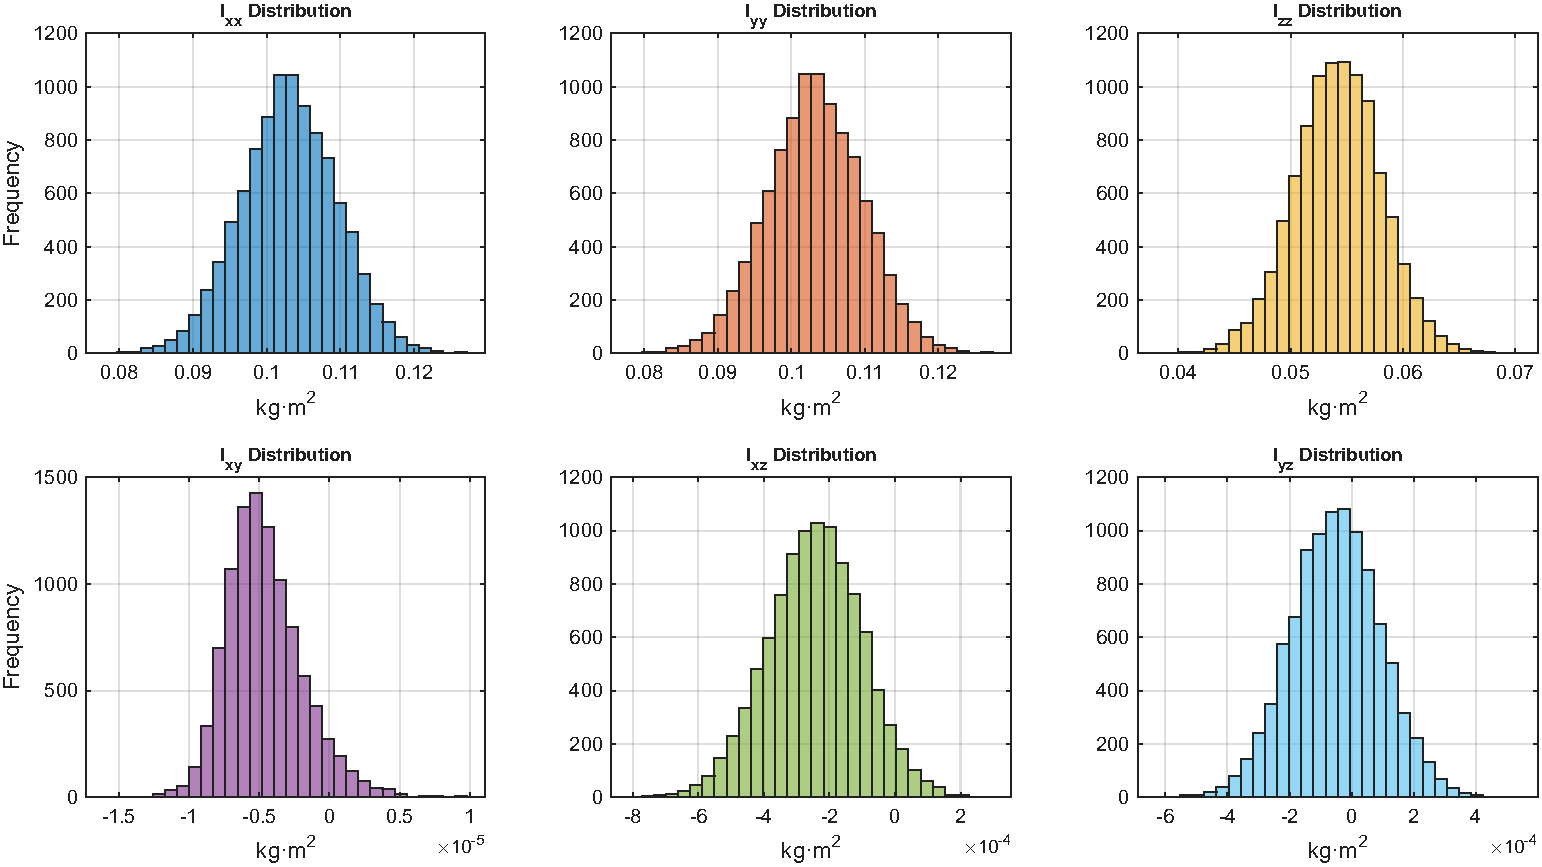
\includegraphics[width=\linewidth]{UCSP_Pictures/SAT-ABC.pdf}
        \caption{SAT-ABC configuration.}
        \label{fig:montecarlos_SATABC}
    \end{subfigure}
    \hfill % Espacio horizontal entre las subfiguras
    % Segunda subfigura (SAT-BC)
    \begin{subfigure}[b]{0.48\linewidth}
        \centering
        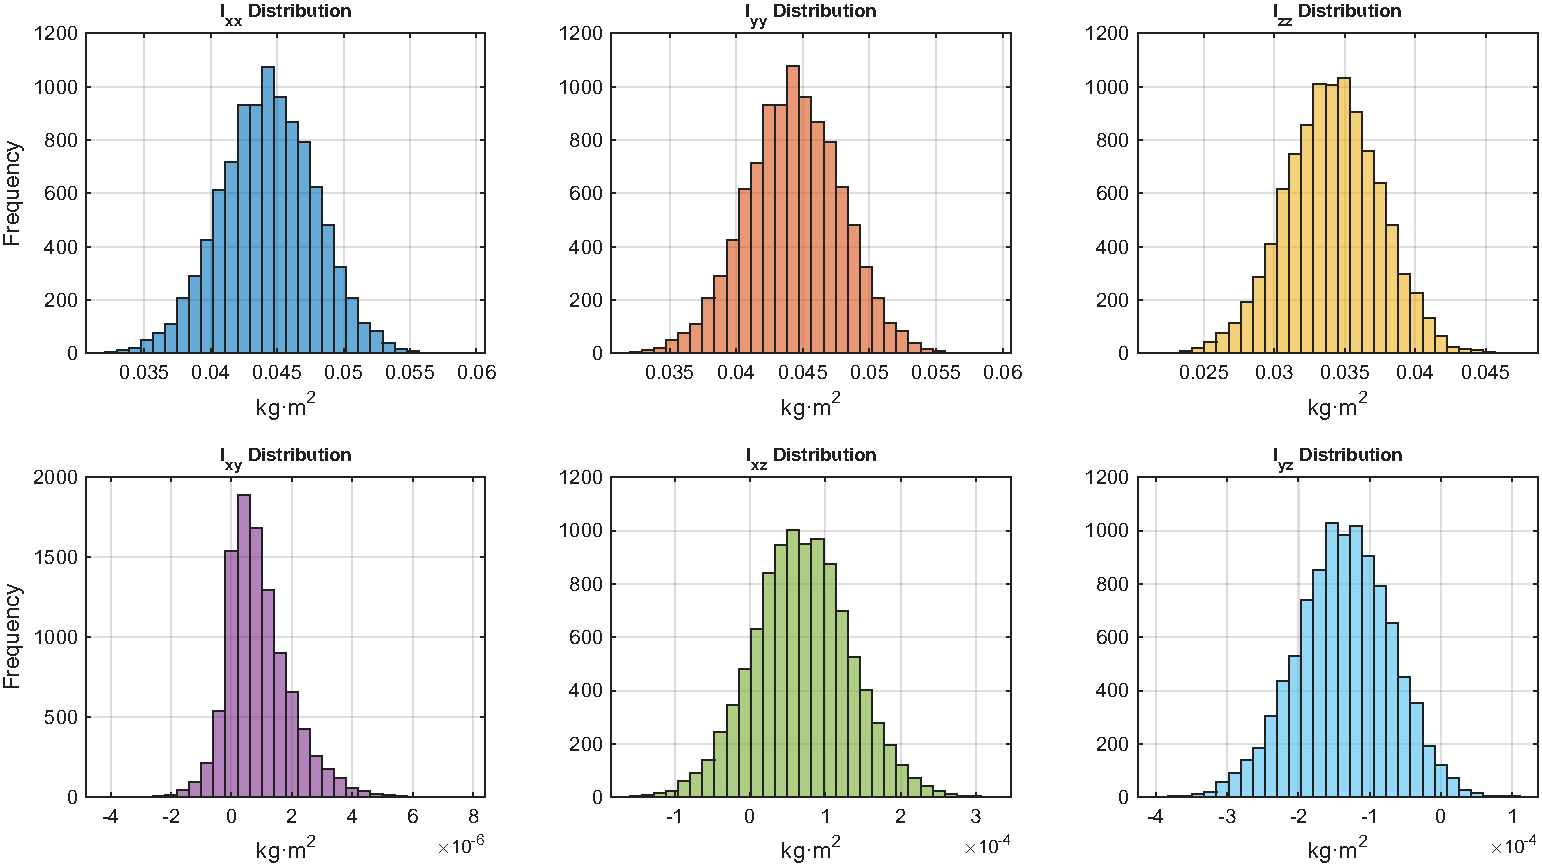
\includegraphics[width=\linewidth]{UCSP_Pictures/SAT-BC.pdf}
        \caption{SAT-BC configuration.}
        \label{fig:montecarlos_SATBC}
    \end{subfigure}
    
    % Caption y Label global del análisis de Montecarlo
    \caption{Monte Carlo analysis for the inertia tensors of different satellite configurations.}
    \label{fig:montecarlo_inertia_analysis}
\end{figure}

\begin{table}[h!]
\centering
\caption{Monte Carlo Statistical Analysis Results ($N=10,000$ Samples)}
\label{tab:monte_carlo_results}
\begin{small}
\begin{tabular}{lcccc}
\hline
\textbf{Parameter} & \textbf{Mean ($\mu$)} & \textbf{Std. Dev. ($\sigma$)} & \textbf{Minimum} & \textbf{Maximum} \\ \hline
\rowcolor[HTML]{EFEFEF} 
\multicolumn{5}{l}{\textit{SAT-ABC (Complete System)}} \\
$I_{xx}$ [kg$\cdot$m$^2$] & $1.0307 \times 10^{-1}$ & $6.5180 \times 10^{-3}$ & $7.8748 \times 10^{-2}$ & $1.2717 \times 10^{-1}$ \\
$I_{yy}$ [kg$\cdot$m$^2$] & $1.0324 \times 10^{-1}$ & $6.5319 \times 10^{-3}$ & $7.8877 \times 10^{-2}$ & $1.2739 \times 10^{-1}$ \\
$I_{zz}$ [kg$\cdot$m$^2$] & $5.4242 \times 10^{-2}$ & $3.8730 \times 10^{-3}$ & $3.8170 \times 10^{-2}$ & $7.0257 \times 10^{-2}$ \\
$I_{xy}$ [kg$\cdot$m$^2$] & $-4.5842 \times 10^{-6}$ & $2.7254 \times 10^{-6}$ & $-1.5333 \times 10^{-5}$ & $9.7442 \times 10^{-6}$ \\
$I_{xz}$ [kg$\cdot$m$^2$] & $-2.4415 \times 10^{-4}$ & $1.4299 \times 10^{-4}$ & $-7.8859 \times 10^{-4}$ & $2.7899 \times 10^{-4}$ \\
$I_{yz}$ [kg$\cdot$m$^2$] & $-5.0079 \times 10^{-5}$ & $1.4272 \times 10^{-4}$ & $-6.0003 \times 10^{-4}$ & $5.2290 \times 10^{-4}$ \\ \hline
\rowcolor[HTML]{EFEFEF} 
\multicolumn{5}{l}{\textit{SAT-BC (Payload Subsystem)}} \\
$I_{xx}$ [kg$\cdot$m$^2$] & $4.4358 \times 10^{-2}$ & $3.5668 \times 10^{-3}$ & $3.0788 \times 10^{-2}$ & $5.8615 \times 10^{-2}$ \\
$I_{yy}$ [kg$\cdot$m$^2$] & $4.4356 \times 10^{-2}$ & $3.5667 \times 10^{-3}$ & $3.0786 \times 10^{-2}$ & $5.8621 \times 10^{-2}$ \\
$I_{zz}$ [kg$\cdot$m$^2$] & $3.4150 \times 10^{-2}$ & $3.3279 \times 10^{-3}$ & $2.1147 \times 10^{-2}$ & $4.8788 \times 10^{-2}$ \\
$I_{xy}$ [kg$\cdot$m$^2$] & $8.9099 \times 10^{-7}$ & $1.0411 \times 10^{-6}$ & $-3.0924 \times 10^{-6}$ & $7.0328 \times 10^{-6}$ \\
$I_{xz}$ [kg$\cdot$m$^2$] & $6.7279 \times 10^{-5}$ & $6.4721 \times 10^{-5}$ & $-1.5532 \times 10^{-4}$ & $3.5186 \times 10^{-4}$ \\
$I_{yz}$ [kg$\cdot$m$^2$] & $-1.3559 \times 10^{-4}$ & $6.6776 \times 10^{-5}$ & $-4.1109 \times 10^{-4}$ & $1.1353 \times 10^{-4}$ \\ \hline
\end{tabular}
\end{small}
\end{table}

\subsubsection{Satellite Orbital propagation}
Satellite orbital propagation for this study was performed using the Orekit suite, which provides numerical orbit propagation, driven by an adaptive variable-step integrator (Dormand–Prince 8(5,3)), which takes into account accelerations produced by the Harris–Priester atmospheric drag, third-body gravitational attraction from the Sun and the Moon, and isotropic solar radiation pressure \cite{maisonobe_2026_18527188}.

The satellite kinematics obtained using the orbital parameters of Table \ref{tab:orbit_params} after a period of 5 hours (3 orbits) are depicted in Figure \ref{fig:satellite_kinematics}.

\begin{table}[ht]
\centering
\caption{Orbital Elements and Mission Environment}
\label{tab:orbit_params}
\begin{tabular}{lll}
\toprule
\textbf{Orbital Element} & \textbf{Value} & \textbf{Unit} \\
\midrule
Semi-major Axis ($a$) & 6992000.0 & {m} \\
Eccentricity ($e$) & 0.0037118 & - \\
Inclination ($i$) & 97.799 & {deg} \\
RAAN ($\Omega$) & 80.477 & {deg} \\
Argument of Perigee ($\omega$) & 65.443 & {deg} \\
True Anomaly ($\nu$) & 294.6817 & {deg} \\
\midrule
Mean Altitude ($h$) & 613863.0 & {m} \\
Orbital Period ($T$) & 5818.5 & {s} \\
Circular Velocity ($v_c$) & 7550.5 & {m/s} \\
\bottomrule
\end{tabular}
\end{table}

\begin{figure}[ht]
    \centering
    % Primera subfigura (Posición)
    \begin{subfigure}[b]{0.48\linewidth}
        \centering
        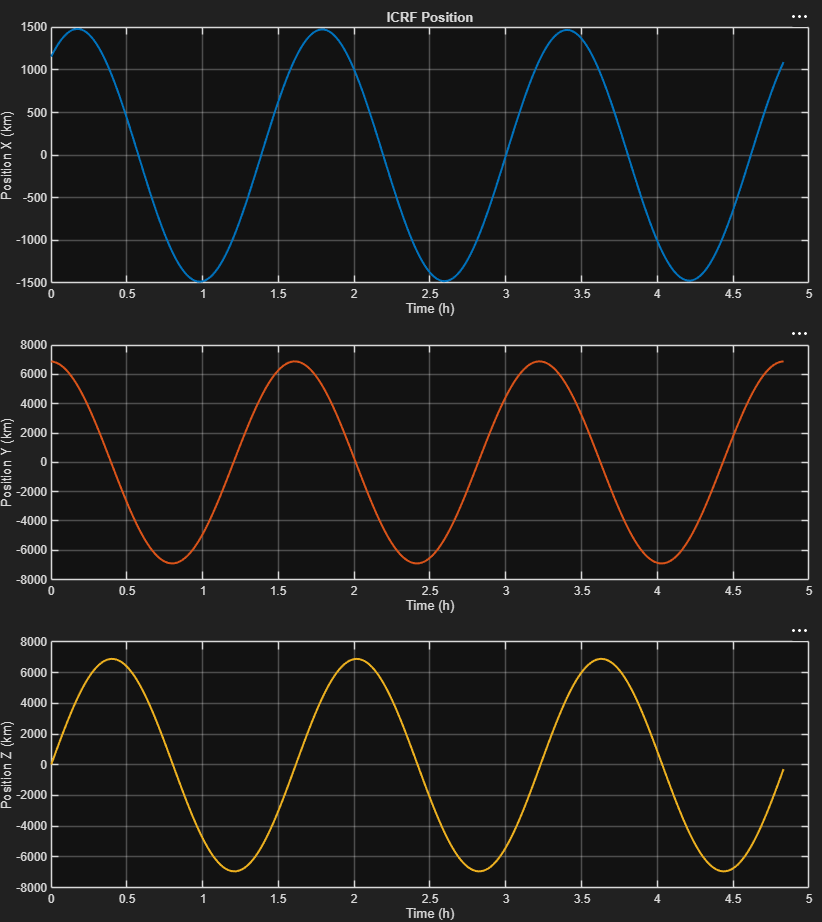
\includegraphics[width=\linewidth]{UCSP_Pictures/satellite_positions_CGRF.png}
        \caption{Satellite positions in CGRF.}
        \label{fig:satellite_positions}
    \end{subfigure}
    \hfill % Espacio horizontal entre las dos imágenes
    % Segunda subfigura (Velocidad)
    \begin{subfigure}[b]{0.48\linewidth}
        \centering
        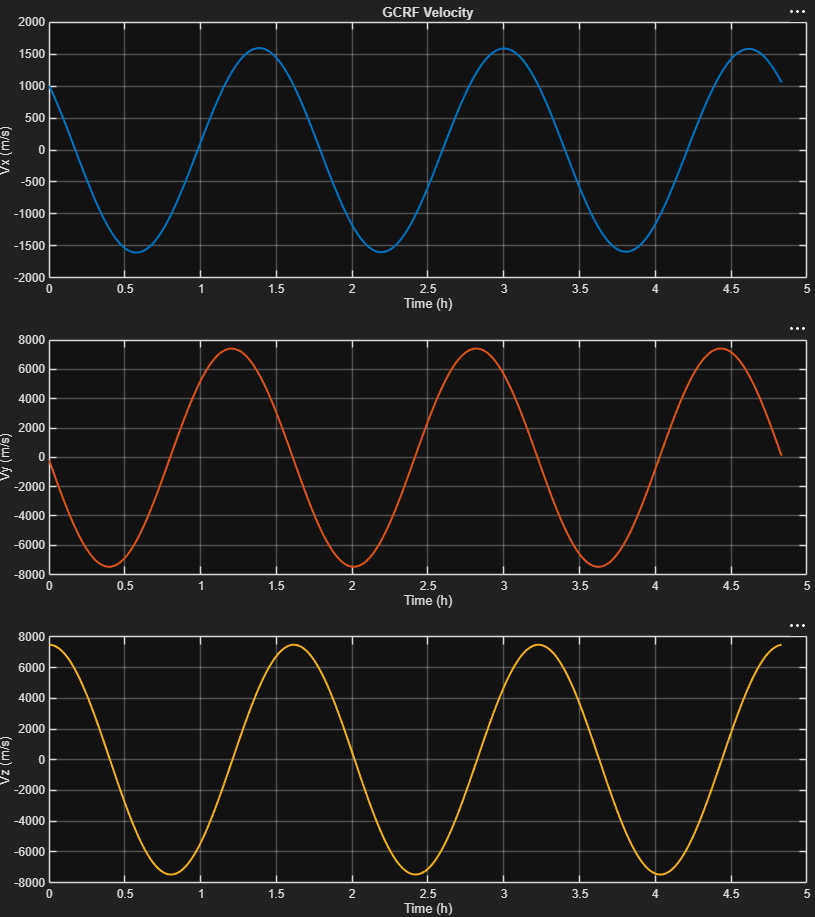
\includegraphics[width=\linewidth]{UCSP_Pictures/satellite_velocity_CGRF.png}
        \caption{Satellite velocity in CGRF.}
        \label{fig:satellite_velocity}
    \end{subfigure}
    
    % Caption y Label global de todo el grupo de figuras
    \caption{Satellite kinematic states during orbital propagation.}
    \label{fig:satellite_kinematics}
\end{figure}

The third-body gravitational accelerations from the Moon and the Sun calculated using the Orekit suite are presented in Figure \ref{fig:third_body_perturbations}.
\begin{figure}[htbp]
    \centering
    % Primera subfigura (Aceleración de la Luna)
    \begin{subfigure}[b]{0.48\linewidth}
        \centering
        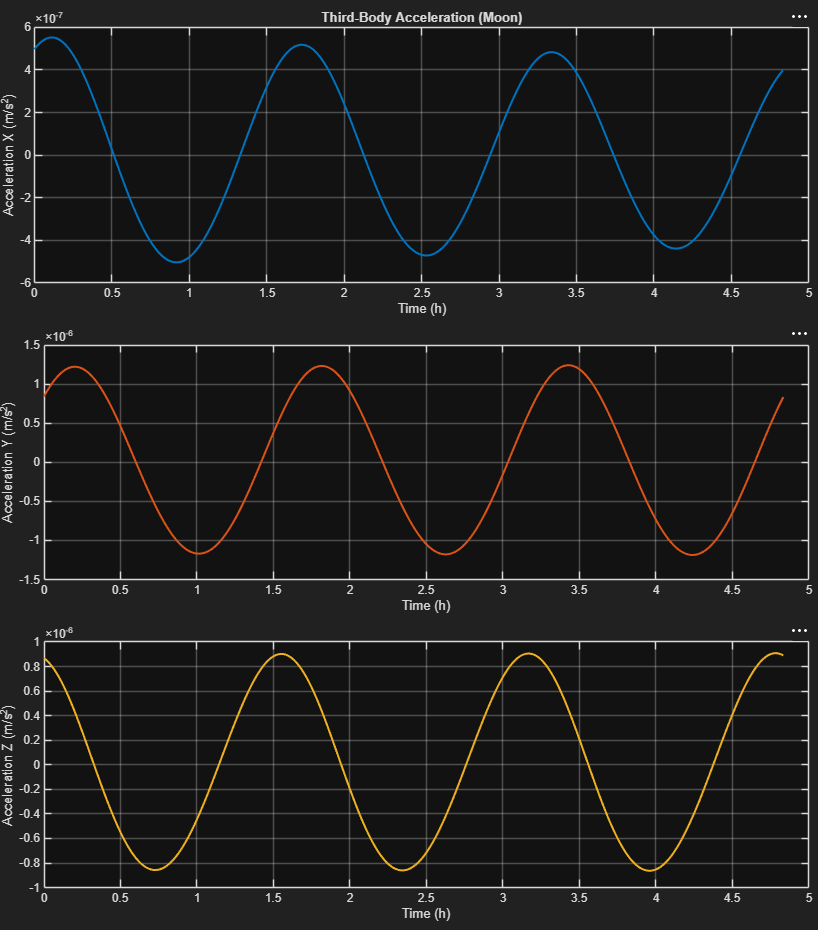
\includegraphics[width=\linewidth]{UCSP_Pictures/moonacceleration.png}
        \caption{Lunar third-body acceleration.}
        \label{fig:moon_acceleration}
    \end{subfigure}
    \hfill % Espacio horizontal entre las subfiguras
    % Segunda subfigura (Aceleración del Sol)
    \begin{subfigure}[b]{0.48\linewidth}
        \centering
        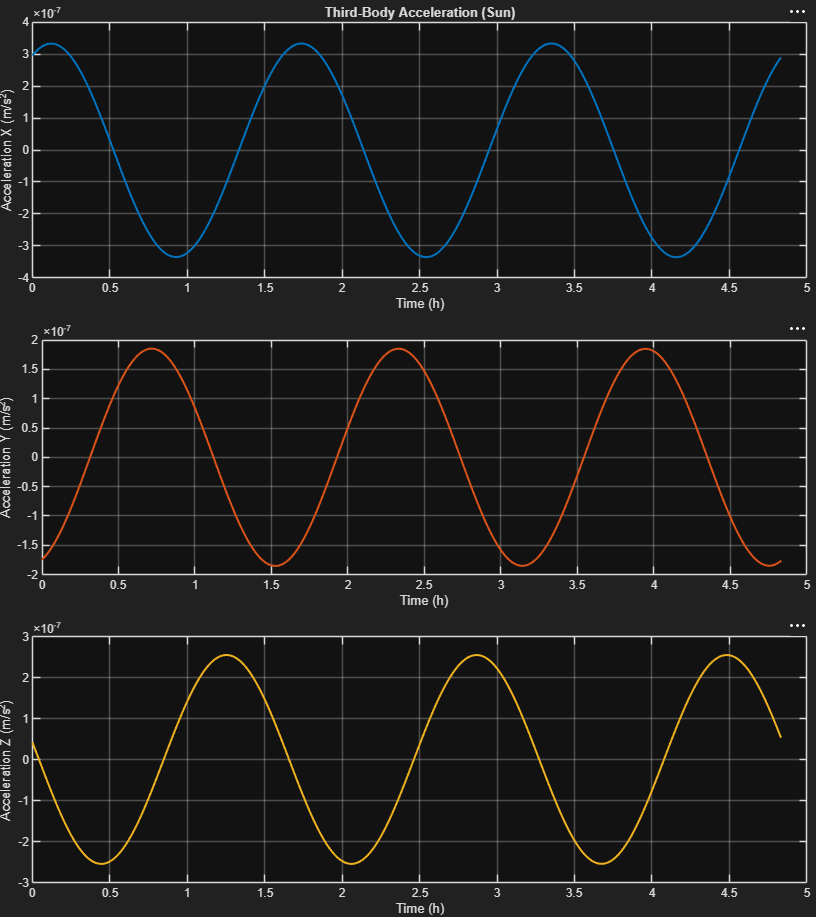
\includegraphics[width=\linewidth]{UCSP_Pictures/sunacceleration.png}
        \caption{Solar third-body acceleration.}
        \label{fig:sun_acceleration}
    \end{subfigure}
    
    % Caption y Label global del bloque
    \caption{Third-body gravitational perturbations acting on the satellite.}
    \label{fig:third_body_perturbations}
\end{figure}


\begin{figure}[htbp]
    \centering
    % Primera subfigura (Presión de Radiación Solar)
    \begin{subfigure}[b]{0.48\linewidth}
        \centering
        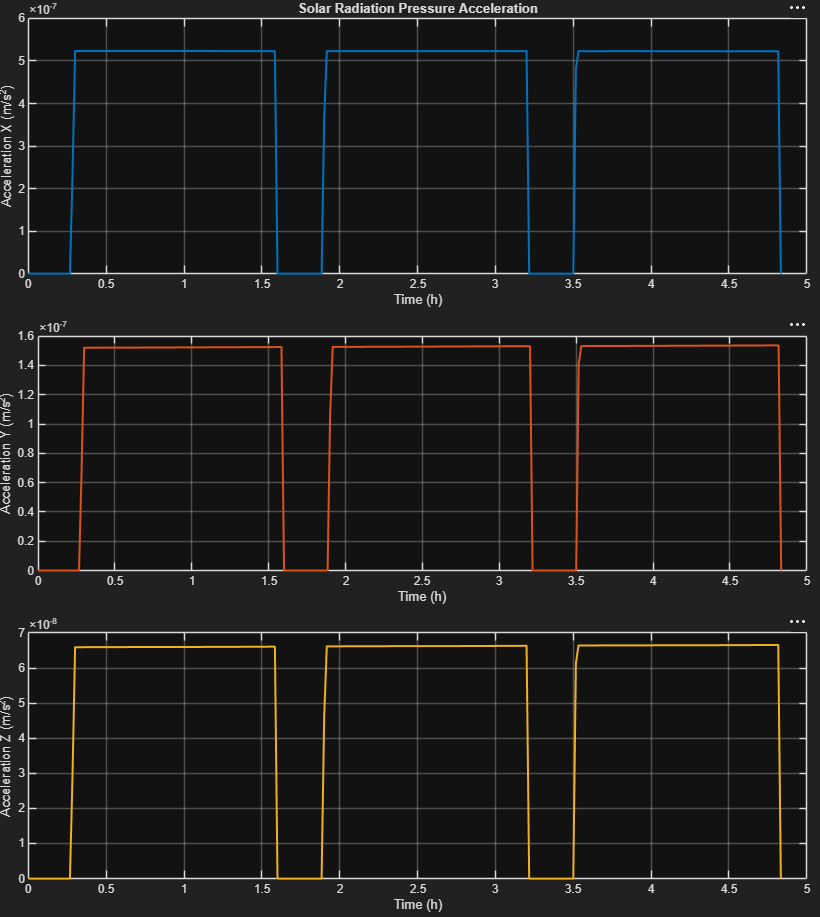
\includegraphics[width=\linewidth]{UCSP_Pictures/solar_rad-acceleration.png}
        \caption{Solar radiation pressure acceleration.}
        \label{fig:solar_radiation_acc}
    \end{subfigure}
    \hfill % Espacio horizontal entre las subfiguras
    % Segunda subfigura (Arrastre Atmosférico)
    \begin{subfigure}[b]{0.48\linewidth}
        \centering
        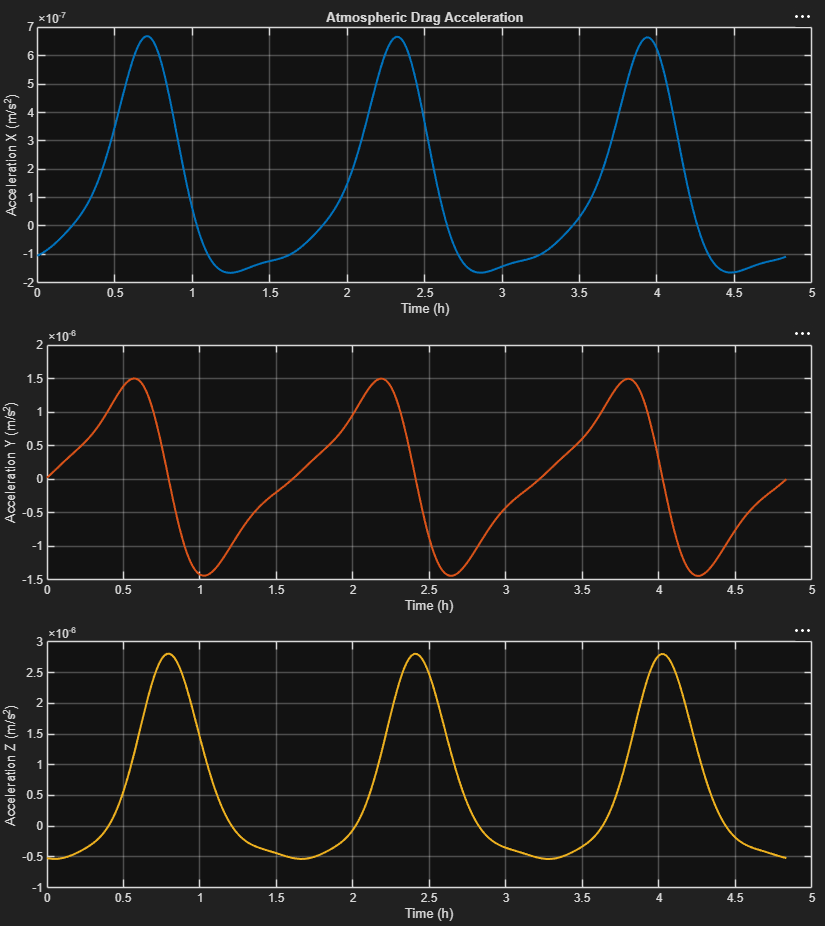
\includegraphics[width=\linewidth]{UCSP_Pictures/satellite_drag_acceleration_CGRF.png}
        \caption{Atmospheric drag acceleration in CGRF.}
        \label{fig:atmospheric_drag_acc}
    \end{subfigure}
    
    % Caption y Label global del bloque de perturbaciones no gravitatorias
    \caption{Non-gravitational acceleration perturbations acting on the satellite.}
    \label{fig:non_gravitational_perturbations}
\end{figure}

It is important to note that since the SAT-ABC and SAT-BC bodies will remain in close proximity during the initial stages of the Linku mission, the same orbital propagation model and environmental accelerations are considered for both spacecraft.

\subsubsection{Reference frames}
The body reference frames used for both simulations are depicted in Figure \ref{fig:sat_abc_body_frame} for SAT-ABC and Figure \ref{fig:sat_bc_body_frame} for SAT-BC, assuming that the origin of both reference frames is located at the center of mass.

\begin{figure}[ht]
    \centering
    % Primera subfigura (SAT-ABC Body Frame)
    \begin{subfigure}[b]{0.38\linewidth}
        \centering
        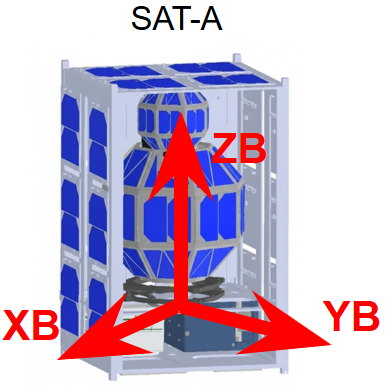
\includegraphics[width=\linewidth]{UCSP_Pictures/sat_abc_body_frame.png}
        \caption{SAT-ABC body fixed reference frame.}
        \label{fig:sat_abc_body_frame}
    \end{subfigure}
    \hspace{1cm} % Espacio horizontal entre las subfiguras
    % Segunda subfigura (SAT-BC Body Frame)
    \begin{subfigure}[b]{0.28\linewidth}
        \centering
        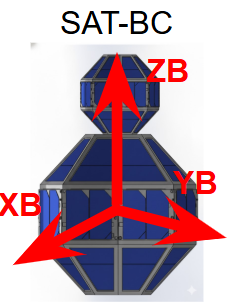
\includegraphics[width=\linewidth]{UCSP_Pictures/sat_bc_body_frame.png}
        \caption{SAT-BC body fixed reference frame.}
        \label{fig:sat_bc_body_frame}
    \end{subfigure}
    
    % Caption y Label global del bloque
    \caption{Definition of body reference frames for different satellite configurations (Images with different scales).}
    \label{fig:satellite_body_frames}
\end{figure}

Figure \ref{fig:satellite_propagation_frames} illustrates the other two reference frames used for the simulation. The GCRF (Geocentric Celestial Reference Frame) was employed as the inertial reference frame. For the orbital LVLH frame, the convention established in previous reports was adopted: the Z-axis points toward nadir, and the X-axis is aligned with the satellite’s velocity vector.

\begin{figure}[htbp]
    \centering
    % Primera subfigura (Propagación orbital)
    \begin{subfigure}[b]{0.48\linewidth}
        \centering
        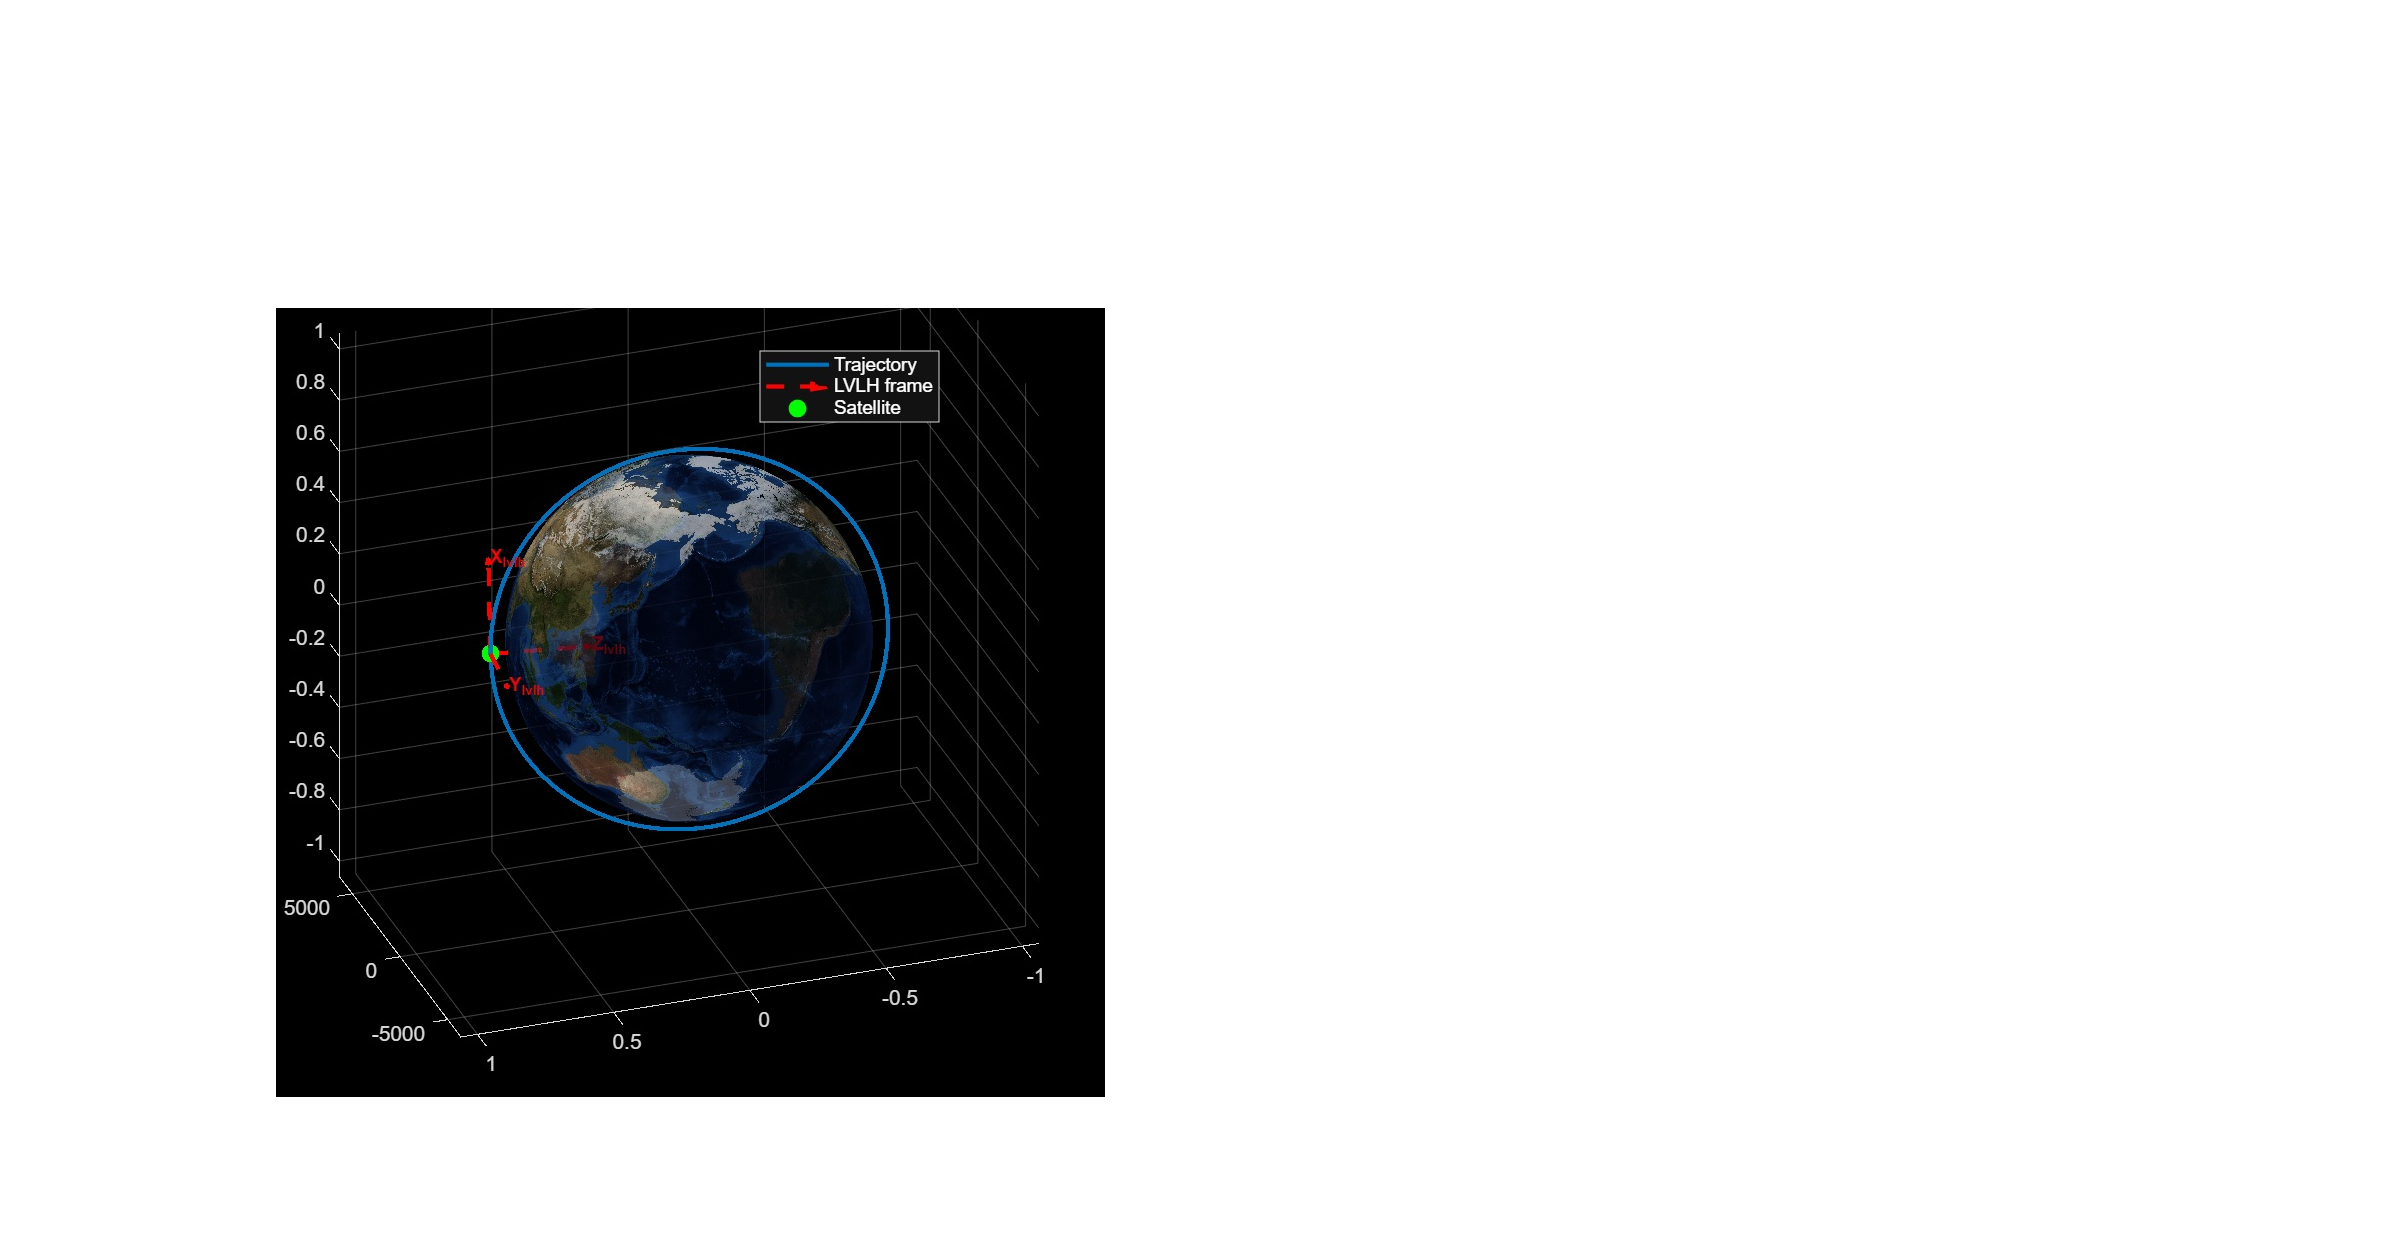
\includegraphics[width=\linewidth]{UCSP_Pictures/satellite-propagation.pdf}
        \caption{Orbital propagation and reference frames.}
        \label{fig:satellite_propagation_frames}
    \end{subfigure}
    \hfill % Espacio horizontal entre las subfiguras
    % Segunda subfigura (Campo magnético)
    \begin{subfigure}[b]{0.48\linewidth}
        \centering
        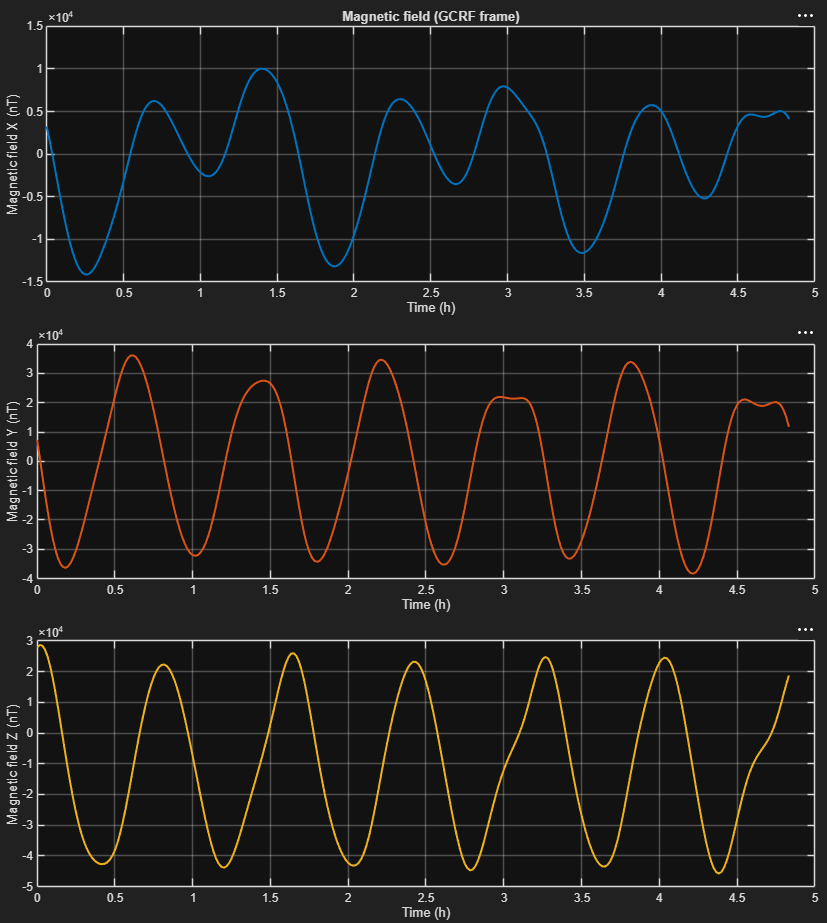
\includegraphics[width=\linewidth]{UCSP_Pictures/magneticfield.png}
        \caption{Geomagnetic field model simulation.}
        \label{fig:magnetic_field_simulation}
    \end{subfigure}
    
    % Caption y Label global del bloque
    \caption{Orbital environment and trajectory simulation obtained using the Orekit suite.}
    \label{fig:orbital_environment_simulation}
\end{figure}

\subsubsection{Geomagnetic Field Model (IGRF)}
The Earth's magnetic field is simulated using the International Geomagnetic Reference Field (IGRF) model, which represents the standard mathematical description of the planet's main magnetic field and its secular variations. In this report, the IGRF coefficients are dynamically evaluated at the satellite's position at each time step and subsequently converted into the inertial frame (GCRF) to remain consistent with the other physical perturbations. The resulting geomagnetic field vector mapped over three orbital periods is presented in Figure \ref{fig:magnetic_field_simulation}.

\subsubsection{Sensor Models}
\begin{enumerate}
    \item \textbf{Inertial Measurement Unit (IMU):}
    The IMU model include scale factor errors ($\mathbf{T}_{\text{sf}}$), axis misalignment ($\mathbf{T}_{\text{ma}}$), and bias instability ($\mathbf{b}_g(t)$) modeled as a random walk process.

    Where $\mathbf{T}_{\text{sf}}$ and $\mathbf{T}_{\text{ma}}$ are defined in \eqref{eq_scaleFactorMatrix}:
    \begin{equation}
        \mathbf{T}_{\text{sf}} = \begin{bmatrix} 1+s_x & 0 & 0 \\ 0 & 1+s_y & 0 \\ 0 & 0 & 1+s_z \end{bmatrix}
        \hspace{0.2cm} \text{and} \hspace{0.2cm}
        \mathbf{T}_{\text{ma}} = \begin{bmatrix} 1 & m_{yx} & m_{zx} \\ m_{xy} & 1 & m_{zy} \\ m_{xz} & m_{yz} & 1 \end{bmatrix},
        \label{eq_scaleFactorMatrix}
    \end{equation}

with $s_x, s_y, s_z$ are the scale factor errors for each axis, and $m_{ij}$ represents the angular deviation of axis $i$ with respect to axis $j$.

The raw gyroscope measurement is given by \eqref{eq_gyro_equation}:
\begin{equation}
    \tilde{\boldsymbol{\omega}}_{\text{raw}}(t) = \mathbf{T}_{\text{ma}} \mathbf{T}_{\text{sf}} \boldsymbol{\omega}(t) + \mathbf{b}_g(t) + \boldsymbol{\eta}_g(t),
    \label{eq_gyro_equation}
\end{equation}
where the time-varying bias $\mathbf{b}_g(t) \in \Re{R}^3$ evolves according to the random walk model:
\begin{equation}
    \mathbf{b}_g(t) = \mathbf{b}_g(t-\Delta t) + \boldsymbol{\eta}_{bg}.
    \label{eq_biasInstability}
\end{equation}
Here, $\boldsymbol{\eta}_{bg}$ is a Gaussian noise process with a standard deviation of $\sigma_{\text{RW}} \sqrt{\Delta t}$. Additionally, a first-order digital low-pass filter is applied to the gyroscope readings to mitigate high-frequency noise, governed by \eqref{eq_gyro_filter}.
\begin{equation}
    \tilde{\boldsymbol{\omega}}_{\text{filt}}(k) = (1 - \alpha) \tilde{\boldsymbol{\omega}}_{\text{filt}}(k-1) + \alpha \tilde{\boldsymbol{\omega}}_{\text{raw}}(k),
    \label{eq_gyro_filter}
\end{equation}
where $\alpha = T_s / (\tau + T_s)$, with $\tau$ being the filter time constant and $T_s$ the sampling time.

Similarly, the accelerometer and magnetometer measurements are expressed in \eqref{eq_acc_measurement_model} and \eqref{eq_mag_measurement_model}, respectively.
\begin{equation}
    \tilde{\mathbf{f}}_{\text{raw}} = \mathbf{T}_{\text{ma}} \mathbf{T}_{\text{sf}} \left( \mathbf{R}(\mathbf{q})^T \mathbf{g}_I \right) + \mathbf{b}_a + \boldsymbol{\eta}_a,
    \label{eq_acc_measurement_model}
\end{equation}
\begin{equation}
    \tilde{\mathbf{m}}_{\text{raw}} = \mathbf{T}_{\text{ma}} \mathbf{T}_{\text{sf}} \left( \mathbf{R}(\mathbf{q})^T \mathbf{m}_I \right) + \mathbf{b}_m + \boldsymbol{\eta}_m.
    \label{eq_mag_measurement_model}
\end{equation}

To account for physical hardware limitations, a saturation and quantization stage is applied to all sensor outputs. The raw physical signal vector $\mathbf{y} \in \Re{R}^3$ is first bounded element-wise by the sensor's operational limits, $y_{\text{min}}$ and $y_{\text{max}}$, yielding the saturated signal vector $\mathbf{y}_{\text{sat}}$. This bounded vector is then mapped to an analog input voltage vector $\mathbf{V}_{\text{in}}$ within the range $[0, V_{\text{ref}}]$ using \eqref{eq_saturation}:
\begin{equation}
    \mathbf{V}_{\text{in}} = \frac{V_{\text{ref}}}{y_{\text{max}} - y_{\text{min}}} \left( \mathbf{y}_{\text{sat}} - y_{\text{min}} \mathbf{1}_{3\times 1} \right).
    \label{eq_saturation}
\end{equation}

Subsequently, $\mathbf{V}_{\text{in}}$ is quantized into an integer digital vector $\mathbf{D}_{\text{out}}$ based on the resolution of an $n_{\text{bits}}$ Analog-to-Digital Converter (ADC), applying the rounding operation element-wise as described in \eqref{eq_adc_digital}.
\begin{equation}
    \mathbf{D}_{\text{out}} = \text{round} \left( \frac{2^{n_{\text{bits}}} - 1}{V_{\text{ref}}} \mathbf{V}_{\text{in}} \right).
    \label{eq_adc_digital}
\end{equation}

Finally, the discrete physical value reintroduced into the simulation, $\mathbf{y}_{\text{out}}$, is reconstructed from the digital integer vector using \eqref{eq_quantization}:
\begin{equation}
    \mathbf{y}_{\text{out}} = y_{\text{min}} \mathbf{1}_{3\times 1} + \frac{y_{\text{max}} - y_{\text{min}}}{2^{n_{\text{bits}}} - 1} \mathbf{D}_{\text{out}},
    \label{eq_quantization}
\end{equation}
where $\mathbf{1}_{3\times 1} = [1, 1, 1]^T$ is a column vector of ones.

\item \textbf{Simple Sun Sensor model:}
The simulation uses a simple sun sensor model modeled as a reference vector. The measurement for the sun ($\tilde{\mathbf{s}}_{\text{meas}}$), is described by \eqref{eq_sunSensor}.
\begin{equation}
    \mathbf{\tilde{s}}_{\text{meas}} = \mathbf{R(q)}^T\mathbf{s}_{I} + \mathbf{b}_{\text{sun}} + \boldsymbol{\eta}_{\text{sun}}
    \label{eq_sunSensor}
\end{equation}
where ($\mathbf{b}_{\text{sun}} \in \Re^3$) and ($\boldsymbol{\eta}_{\text{sun}} \in \Re^3$) are the bias and gaussian noise and $\mathbf{s}_{I} \in \Re{R}^3$ is the true line-of-sight vector to the sun, expressed in the inertial frame.
\end{enumerate}

\paragraph{\textbf{Actuator Models}}
\begin{enumerate}
\item \textbf{Reaction Wheel Assembly Model:}
A mathematical model for an array of $N$ reaction wheels (rw). This model encompasses a closed-loop Proportional-Integral-Derivative (PID) speed controller coupled with the electrical and mechanical dynamics of a DC motor, as described by \eqref{eq_rw_mechanical} and \eqref{eq_rw_electrical} for the $j$-th wheel.

\begin{align}
    \dot{\omega}_{\text{rw},j} &= \frac{1}{J_{\text{rw}}} \left( k_t i_j - B \omega_{\text{rw},j} - K_c \text{sign}(\omega_{\text{rw},j}) \right) \label{eq_rw_mechanical} \\
    \dot{i}_j &= \frac{1}{L} \left( u_j - R i_j - K_e \omega_{\text{rw},j} \right) \label{eq_rw_electrical}
\end{align}

where $\omega_{\text{rw},j}$ and $i_j$ are the angular rate and current of the $j$-th reaction wheel. Assuming all wheels are identical, the shared parameters are defined as:
\begin{itemize}
    \item $L, R$: Armature inductance and resistance.
    \item $K_e, K_t$: Back-EMF and motor torque constants.
    \item $J_{\text{rw}}$: Rotor inertia.
    \item $B, K_c$: Viscous and Coulomb friction coefficients.
\end{itemize}

The internal PID controller tracks the reference speed to compute an unbounded voltage $\mathbf{u}_{\text{unb}}$, which is then saturated to $\mathbf{u}_{\text{app}} \in [-V_{\text{max}}, V_{\text{max}}]$ using a clamping anti-windup mechanism. To ensure numerical stability, the motor dynamics in \eqref{eq_rw_electrical} and \eqref{eq_rw_mechanical} are solved via a 4th-order Runge-Kutta (RK4) method. The resulting state vector $\mathbf{x} = [\omega_{rw,j}, i_{rw,j}]^T$ is strictly constrained by the motor's physical limits, $\omega_{\text{rw-max}}$ and $i_{\text{rw-max}}$. Finally, the true mechanical torque exerted by the $j$-th wheel is derived from its momentum rate of change \eqref{eq_rate_of_change}.
\begin{equation}
    \tau_{\text{real}, j} = J_{\text{rw}} \frac{\omega_{rw,j}(t) - \omega_{rw,j}(t-\Delta t)}{\Delta t},
    \label{eq_rate_of_change}
\end{equation}
which is subsequently projected onto the satellite's body frame using the actuator configuration matrix $\mathbf{W_{rw}}$.

\item \textbf{Magnetorquer Assembly Model:}
A mathematical model for a set of $N$ magnetorquers, mapping the commanded magnetic dipole to the true mechanical torque while accounting for both magnetic and electrical constraints. First, the commanded dipole vector $\mathbf{m}_{\text{cmd}} \in \Re{R}^N$ is bounded by the physical saturation limit of the magnetic core, $\mathbf{m}_{\text{sat}} \in [-m_{\text{max}}, m_{\text{max}}]$.

To model Electrical Power System (EPS) limitations, the required coil voltage is computed using Ohm's law, $\mathbf{V}_{\text{req}} = (\mathbf{m}_{\text{sat}}/K_m)R_m$, where $R_m$ is the internal resistance and $K_m$ is the current-to-dipole conversion factor (assuming all magnetorquers equal). This required voltage is subsequently limited by the maximum power bus voltage, $V_{\text{max}}$, to obtain the actual applied voltage $\mathbf{V}_{\text{app}} \in [-V_{\text{max}}, V_{\text{max}}]$:

Consequently, the realized true dipole $\mathbf{m}_{\text{real}} = K_m (\mathbf{V}_{\text{app}}/R_m)$ is inherently bounded by these cascaded saturation stages. Finally, the individual coil dipoles are mapped to the satellite's body frame using the configuration matrix $\mathbf{W_{mtq}} \in \Re{R}^{3 \times N}$. The resulting control torque $\boldsymbol{\tau}_{\text{mtq}}$ is generated via the cross product with the local geomagnetic field $\mathbf{B}_{\text{body}}$:
\begin{equation}
    \boldsymbol{\tau}_{\text{mtq}} = (\mathbf{W_{mtq}} \mathbf{m}_{\text{real}}) \times \mathbf{B}_{\text{body}}.
    \label{eq_mtq_torque}
\end{equation}
\end{enumerate}


\paragraph{\textbf{Torque disturbances in LEO orbit Analisys}}
To simulate a realistic Low Earth Orbit (LEO) environment, three external torque disturbance sources were implemented considering gravity gradient $\mathbf{T_{gg}}\in \Re_{3\times 3}$, atmospheric drag $\mathbf{T_{drag}}\in \Re_{3\times 3}$, and solar radiation pressure $\mathbf{T_{srp}} \in \Re_{3\times 3}$ using the parameters showed in Tables \ref{tab:orbit_params} and \ref{tab:disturbance_params} assuming the worst possible scenarios. These torques are illustrated in Figure \ref{fig:sat_abc_disturbances} for a span of 100 orbits and in Figure \ref{fig:total_torque_disturbances} for a span of three orbits, assuming SAT-ABC as a free-rotating rigid body and using Orekit solar radiation and drag acceleration models. A summary of the simulation results is shown in Table \ref{tab:disturbances}.

\begin{table}[ht]
\centering
\caption{Environmental disturbance parameters and surface properties for SAT-ABC.}
\label{tab:disturbance_params}
\begin{tabular}{lcl}
\hline
\textbf{Parameter} & \textbf{Value} & \textbf{Description} \\ \hline
$A_{x\pm}, A_{y\pm}$ & 0.06 m$^2$ & Side face areas ($0.2 \times 0.3$ m) \\
$A_{z\pm}$           & 0.04 m$^2$ & Top/Bottom face areas ($0.2 \times 0.2$ m) \\
$q_{ref}$            & 0.62       & Reflectivity coefficient (Al 6061-T6) \\
$C_d$                & 2.2        & Aerodynamic drag coefficient \\
$\mathbf{r}_{cp-cg}$ & $[0.01, -0.005, 0.02]^T$ m & CoP to CoG offset vector \\ \hline
\end{tabular}
\end{table}

\begin{figure}[htbp]
    \centering
    % Primera subfigura (Componentes detallados para SAT-ABC)
    \begin{subfigure}[b]{0.9\linewidth}
        \centering
        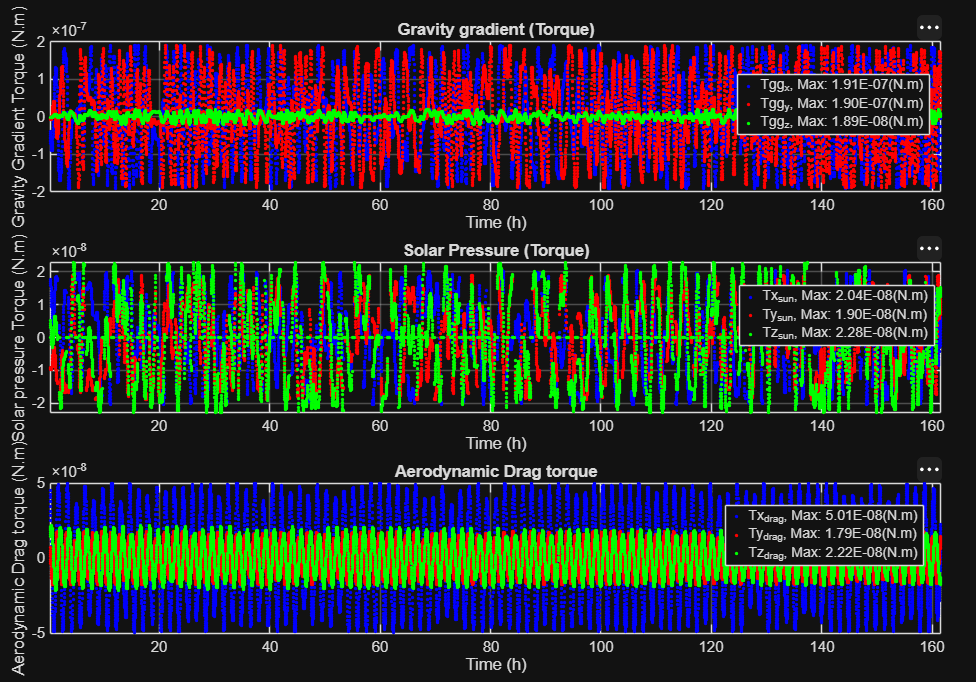
\includegraphics[width=\linewidth]{UCSP_Pictures/Torque_disturbances_v1.png}
        \caption{Environmental disturbances for SAT-ABC.}
        \label{fig:sat_abc_disturbances}
    \end{subfigure}
    % \hfill % Espacio horizontal entre las subfiguras
    % Segunda subfigura (Torque Total)
    \\ % <--- CORRECCIÓN: Salto de línea para forzar la alineación vertical
    \vspace{0.5cm} % Opcional: Agrega un poco de espacio vertical limpio entre ambas
    \begin{subfigure}[b]{0.8\linewidth}
        \centering
        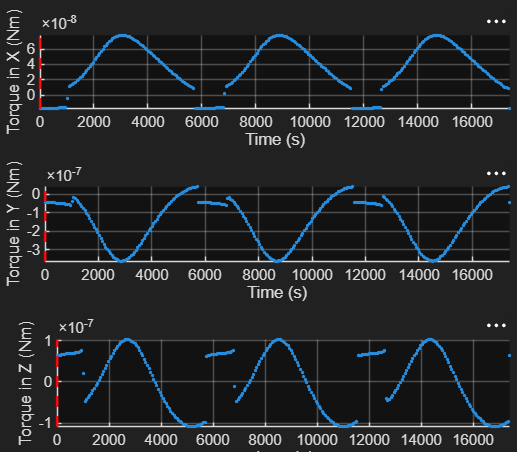
\includegraphics[width=\linewidth]{UCSP_Pictures/Torque_disturbances.png}
        \caption{Total disturbance torque for SAT-ABC, excluding gravity gradient.}
        \label{fig:total_torque_disturbances}
    \end{subfigure}
    
    \caption{Analysis of environmental disturbance torques acting on the spacecraft.}
    \label{fig:environmental_torque_analysis}
\end{figure}


\begin{table}[ht]
\centering
\caption{Maximum Disturbance Torques for the SAT-ABC Configuration}
\label{tab:disturbances}
\begin{tabular}{l c c c c}
\toprule
\textbf{Torque} & \textbf{Max $T_x$ (Nm)} & \textbf{Max $T_y$ (Nm)} & \textbf{Max $T_z$ (Nm)} & \textbf{Mag (Nm)} \\
\midrule
Gravity Gradient   & $1.91 \times 10^{-7}$ & $1.90 \times 10^{-7}$ & $1.90 \times 10^{-8}$ & $2.70 \times 10^{-7}$ \\
Solar Pressure     & $9.94 \times 10^{-9}$ & $1.25 \times 10^{-8}$ & $1.67 \times 10^{-8}$ & $2.31 \times 10^{-8}$ \\
Aerodynamic Torque & $1.47 \times 10^{-8}$ & $4.85 \times 10^{-8}$ & $4.98 \times 10^{-8}$ & $7.10 \times 10^{-8}$ \\
\textbf{Total}     & $\mathbf{2.16 \times 10^{-7}}$ & $\mathbf{2.51 \times 10^{-7}}$ & $\mathbf{8.55 \times 10^{-8}}$ & $\mathbf{3.42 \times 10^{-7}}$ \\
\bottomrule
\end{tabular}
\end{table}

\subsection{Stage I: Integrated Body (SAT-ABC)}
A complete description of the phases which implies the SAT-ABC bodies are described below: 

\subsubsection{Phase 1: Release and System Initialization} 
\begin{itemize}
    \item \textbf{Power-On Self-Test (POST):} The system verifies the electrical and structural integrity of the ADCS sensors and actuators to ensure no damage was sustained from the high-magnitude vibration loads experienced during the launch vehicle's ascent.
    \item \textbf{Sensor Calibration and Biasing:} Biasing and noise characterization are performed during the initial free-drift state. The gyroscopes and magnetometers are calibrated using Extended Kalman Filters (EKF) and sphere-fitting algorithms to identify constant biases and hard-iron displacements, ensuring high-fidelity attitude estimation.
    \item \textbf{Reference Frame Synchronization and Parameter Identification:} The 12U CubeSat's geometric axes are mapped within the flight software. This step involves a passive estimation of the inertia tensor and Center of Mass (CoM) migration by comparing the satellite's response to environmental disturbances against theoretical models based on Euler’s equations for rigid body dynamics.
    \item \textbf{Initial Attitude Determination:} A coarse orientation is resolved by implementing the TRIAD algorithm, which processes solar and magnetic field vectors to establish a stable baseline attitude before initiating the Phase 2 detumbling maneuver.
\end{itemize}

\subsubsection{Phase 2: Detumbling Phase for SAT-ABC}

The detumbling phase for SAT-ABC is executed by an orthogonal array of magnetorquers based on the commercial iADCS400 module. To reduce the satellite's initial high tumble rates (up to $\pm 5$ deg/s) to a stable state ($< 1$ deg/s), a Pure B-Dot controller is employed, as defined in \eqref{eq:b_dot_controller}:

\begin{equation}
    \dot{\mathbf{B}}_{analytical} = -\boldsymbol{\omega}_{meas} \times \mathbf{B}_{meas}
    \label{eq:b_dot_controller}
\end{equation}

The resulting magnetic dipole command is expressed in \eqref{eq:magnetic_dipole_controller}:
\begin{equation}
    \mathbf{M}_{cmd} = -K_{bdot} \cdot f_{bang-bang} \cdot \dot{\mathbf{B}}_{analytical}
    \label{eq:magnetic_dipole_controller}
\end{equation}

The theoretical base gain, $K_{bdot}$, is calculated according to \eqref{eq:b_dot_gain}:
\begin{equation}
    K_{bdot} = \frac{4\pi (1+\sin(i)) I_{min}}{T_{orb} B_{avg}^2}
    \label{eq:b_dot_gain}
\end{equation}

This gain is scaled by a \textit{Bang-Bang Factor} ($f_{bang-bang} = 10^3$) to ensure that braking occurs within the coils' saturation zone, thereby maximizing rotational energy dissipation. Once the stability threshold is reached, The transition logic incorporates a Schmidt trigger (hysteresis) approach to ensure system robustness. The stabilization threshold is set at $\omega_{th} < 1$ deg/s. However, to prevent premature transitions or "chattering" caused by magnetometer noise or instantaneous peaks in the angular velocity, a reset threshold is established at $1.2$ deg/s.

To verify the feasibility of the proposed algorithms, actuators, and sensors, a series of Monte Carlo simulations were performed using the parameters detailed in Table \ref{tab:satellite_parameters}.

\begin{table}[ht]
\centering
\caption{Nominal Parameters for Linku-SAT (12U)}
\label{tab:satellite_parameters}
\small
\begin{tabular}{lll}
\toprule
\textbf{Parameter} & \textbf{Symbol / Variable} & \textbf{Value / Unit} \\ \midrule
\rowcolor[HTML]{EFEFEF} 
%\multicolumn{3}{l}{\textbf{Mechanical Properties}} \\
%Total Mass & $m_{sat}$ & 20.0 kg \\
%Principal Moments of Inertia & $I_{xx}, I_{yy}, I_{zz}$ & 0.278, 0.279, 0.170 $kg \cdot m^2$ \\
%Products of Inertia & $I_{xy}, I_{xz}, I_{yz}$ & -0.005, 0.003, 0.004 $kg \cdot m^2$ \\ \midrule
%\rowcolor[HTML]{EFEFEF} 
\multicolumn{3}{l}{\textbf{Actuators: Magnetorquers (based on the iADCS400)}} \\
Maximum Power & $P_{max}$ & 600 mW \\
Operating Voltage & $V_{op}$ & 5 V \\
Nominal Magnetic Dipole & $m_{nom}$ & 0.4 $A \cdot m^2$ \\
Residual Dipole (Remanence) & $\mathbf{M}_{rem}$ & $[0.004, -0.002, 0.003]^T$ $A \cdot m^2$ \\
Linearity Factor (Core) & $k_{lin}$ & 2.0 (dimensionless) \\ \midrule
\rowcolor[HTML]{EFEFEF} 
\multicolumn{3}{l}{\textbf{Sensors: IMU (Mag + Gyro) (based on the iADCS400)}} \\
Magnetometer Std. Deviation & $\sigma_{mag}$ & 150 nT \\
Magnetometer Resolution & $res_{mag}$ & 10 nT \\
Gyroscope Noise & $\eta_{gyro}$ & 0.05 deg/s \\
Bias Random Walk & $\sigma_{RW}$ & 0.005 $deg/s/\sqrt{s}$ \\
Gyro Saturation Range & $\omega_{max}$ & $\pm$ 250 deg/s \\ \midrule
%\rowcolor[HTML]{EFEFEF} 
%\multicolumn{3}{l}{\textbf{Orbital Parameters (LEO SSO)}} \\
%Semi-major Axis & $a$ & 6992 km \\
%Inclination & $i$ & 97.799$^\circ$ \\
%Eccentricity & $e$ & 0.0037 \\
%Orbital Period & $T$ & $\sim$ 5815 s \\ \midrule
%\rowcolor[HTML]{EFEFEF} 
%\multicolumn{3}{l}{\textbf{Control Configuration}} \\
%PID Gains & $K_p, K_i, K_d$ & $8 \cdot 10^{-5}, 5 \cdot 10^{-5}, 3 \cdot 10^{-3}$ \\
%Detumbling Threshold & $\omega_{th}$ & 1 deg/s \\
%Anti-Windup Limit & $limit_{int}$ & 50 \\ \bottomrule
\end{tabular}
\end{table}

\begin{figure}
    \centering
    \includegraphics[width=0.9\linewidth]{UCSP_Pictures/State 1 Verification.pdf}
    \caption{Monte Carlo simulation results for the detumbling phase of SAT-ABC: angular velocity convergence and settling time distributions.}
    \label{fig:monte_carlo_results}
\end{figure}

Figure \ref{fig:monte_carlo_results} illustrates the evolution of the angular velocity magnitude and the statistical distribution of the settling times.

\begin{itemize}
    \item \textbf{Convergence Rate:} A 100\% success rate was achieved, with 500 out of 500 runs reaching the stabilization threshold ($< 1$ deg/s).
    \item \textbf{First Crossing Time:} The initial crossing of the threshold occurs at a mean time of \textbf{0.55 h}. The bimodal distribution in the "First crossings" histogram suggests two primary convergence behaviors depending on the initial kinetic energy and the orbital magnetic field alignment.
    \item \textbf{Verified Detumbling Time:} To ensure stability, a mandatory \textit{Hold-time} of 3600 s (1.0 h) was implemented. The "Verified runs" analysis shows that the satellite achieves a fully stable state within a mean time of \textbf{1.55 h}, with a worst-case scenario (maximum time) of \textbf{1.92 h}.
    \item \textbf{Robustness against Resets:} The "Hold-time and reset effect" histogram validates that the verification delay remains tightly grouped around the 1.0 h mark, confirming that the hysteresis logic (Reset at 1.2 deg/s) effectively prevents premature transitions due to sensor noise or residual dipoles.
\end{itemize}
The results demonstrate that the SAT-ABC will achieve a stable state in less than  1.3 orbits (considering a $\sim$96 min orbit), providing a significant safety margin for subsequent operational phases such as nominal alignment.

\subsubsection{Phase 3: SAT-ABC Settling mode} 
This phase allows the attitude determination algorithm to reach convergence using an IMU in conjunction with a start tracker modeled as a set of 5 vectors based on the iADCS400 model. This study proposes six AHRS algorithms listed below:
\begin{itemize}
    \item \textbf{QUEST Algorithm:} It is a deterministic algorithm to solve the Wahba's problem by constructing Davenport's K-matrix from weighted body-frame observations and their corresponding inertial references. The implementation computes the gain matrix $B$ and the error vector $z$ to assemble a symmetric $4 \times 4$ matrix, where the eigenvector associated with the largest eigenvalue yields the optimal attitude quaternion. As a "measurement-only" solver, it provides a robust, geometrically-derived orientation estimate independent of gyroscope data, ensuring numerical stability through matrix symmetrization and quaternion normalization \cite{crassidis2021spacecraft, bar1996request}.
    \item \textbf{RE-QUEST Algorithm:} It is the recursive version of QUEST, which evolves the attitude estimation by propagating Davenport’s K-matrix over time using gyroscope measurements and updating it with vector observations. The algorithm maintains an accumulated matrix $K_{acc}$ and a total weight $m_{acc}$, applying a fading memory factor $P$ to prioritize recent data. During the Predict stage, the matrix is propagated via a transition matrix $\Phi$ derived from angular rates, while the Update stage blends the current measurement batch into the existing estimate. The optimal quaternion is then extracted as the principal eigenvector of the updated K-matrix, providing a filter-like behavior that effectively fuses high-frequency rate data with low-frequency reference vectors \cite{bar1996request}.
    \item \textbf{Mahony Filter:} It is a nonlinear complementary filter that estimates spacecraft attitude by fusing high-rate gyroscope data with vector observations through a proportional-integral (PI) feedback mechanism. The algorithm computes an attitude error by comparing measured body-frame vectors with predicted directions derived from the current estimate and inertial references. This error is processed through a proportional gain $K_P$ for immediate orientation correction and an integral gain $K_I$ to dynamically estimate and compensate for gyroscope bias. By operating directly on the Special Orthogonal Group $SO(3)$ via quaternions, the Mahony filter ensures high computational efficiency and global stability, making it ideal for resource-constrained embedded systems \cite{10850038}.
    \item \textbf{Madgwick Filter:} The Madgwick Filter estimates the attitude quaternion ($\mathbf{q}_{est,t}$) and the gyroscope bias ($\mathbf{b_{g,est}}$). This filter, based on the gradient-descent algorithm, fuses high-frequency measurements from $\tilde{\boldsymbol{\omega}}_{meas}$ with low-frequency corrections from $\tilde{\mathbf{f}}_{\text{meas}}$, $\tilde{\mathbf{m}}_{\text{meas}}$, and, optionally, $\mathbf{\tilde{s}}_{\text{meas},n}$. The process is divided into two steps: first, a prediction stage that integrates $\tilde{\boldsymbol{\omega}}_{meas}$ to update $\mathbf{q}_{est,t} = \mathbf{q}_{\omega,t}$ using the kinematics equation \eqref{eq_Kinematics_equation}. Next, a correction stage uses a gradient-descent algorithm to minimize the error between reference vectors and their corresponding measurements. This error is computed as the gradient ($\boldsymbol{\nabla}\mathbf{f}$) of an objective function, which is then normalized to find the direction of the gyroscope error ($\mathbf{\dot{q}}_{\epsilon,t}$). The final rate of change of the orientation is calculated by fusing both estimates as shown in \eqref{eq_estimated_rate}, where $\beta$ is the filter gain.
    \begin{equation}
        \mathbf{\dot{q}}_{\text{est},t} = \mathbf{\dot{q}}_{\omega,t} - \beta \mathbf{\dot{q}}_{\epsilon,t}
         \label{eq_estimated_rate}
    \end{equation}
    The key differences from the original Madgwick implementation are its modular structure, which separates the logic into Predict and Update methods, enabling high-frequency attitude propagation and the algorithm's extension to incorporate star tracker measurements, which improves accuracy by adding more reference vectors to the objective function \cite{madgwick2010filter}.

    \item \textbf{Extended Kalman Filter (EKF):} The  EKF method is well-suited for non-linear systems. The implementation is a full-state filter based on the configuration from \cite{ahrs_ekf, 11121164}, where the state vector is defined as $\mathbf{x} = [\mathbf{q}^T, \mathbf{b}_{\text{g}}^T]^T$, and its uncertainty is managed by the covariance matrix ($\mathbf{P} \in \Re^{7\times 7}$). The measurement model is defined by $\mathbf{y = R(q)^T v_{ref}}$ where $v_{ref}$ represents the reference vectors in the inertial frame. This model is extended by incorporating measurements from a star tracker to improve accuracy. A key architectural feature is the separation into distinct predict and correct stages as depicted in Figure \ref{fig:ekf_processs}. This design enables high-frequency attitude propagation, while the correction step applies updates only when new sensor measurements are available. The correction is performed via an additive update ($\mathbf{x}_{\text{t}} = \mathbf{x}_{{t - \Delta t}} + \mathbf{K} \cdot (y_{meas}-y_{est})$), which requires a subsequent re-normalization of the quaternion component of the state.

    \begin{figure}[ht]
    \centering
    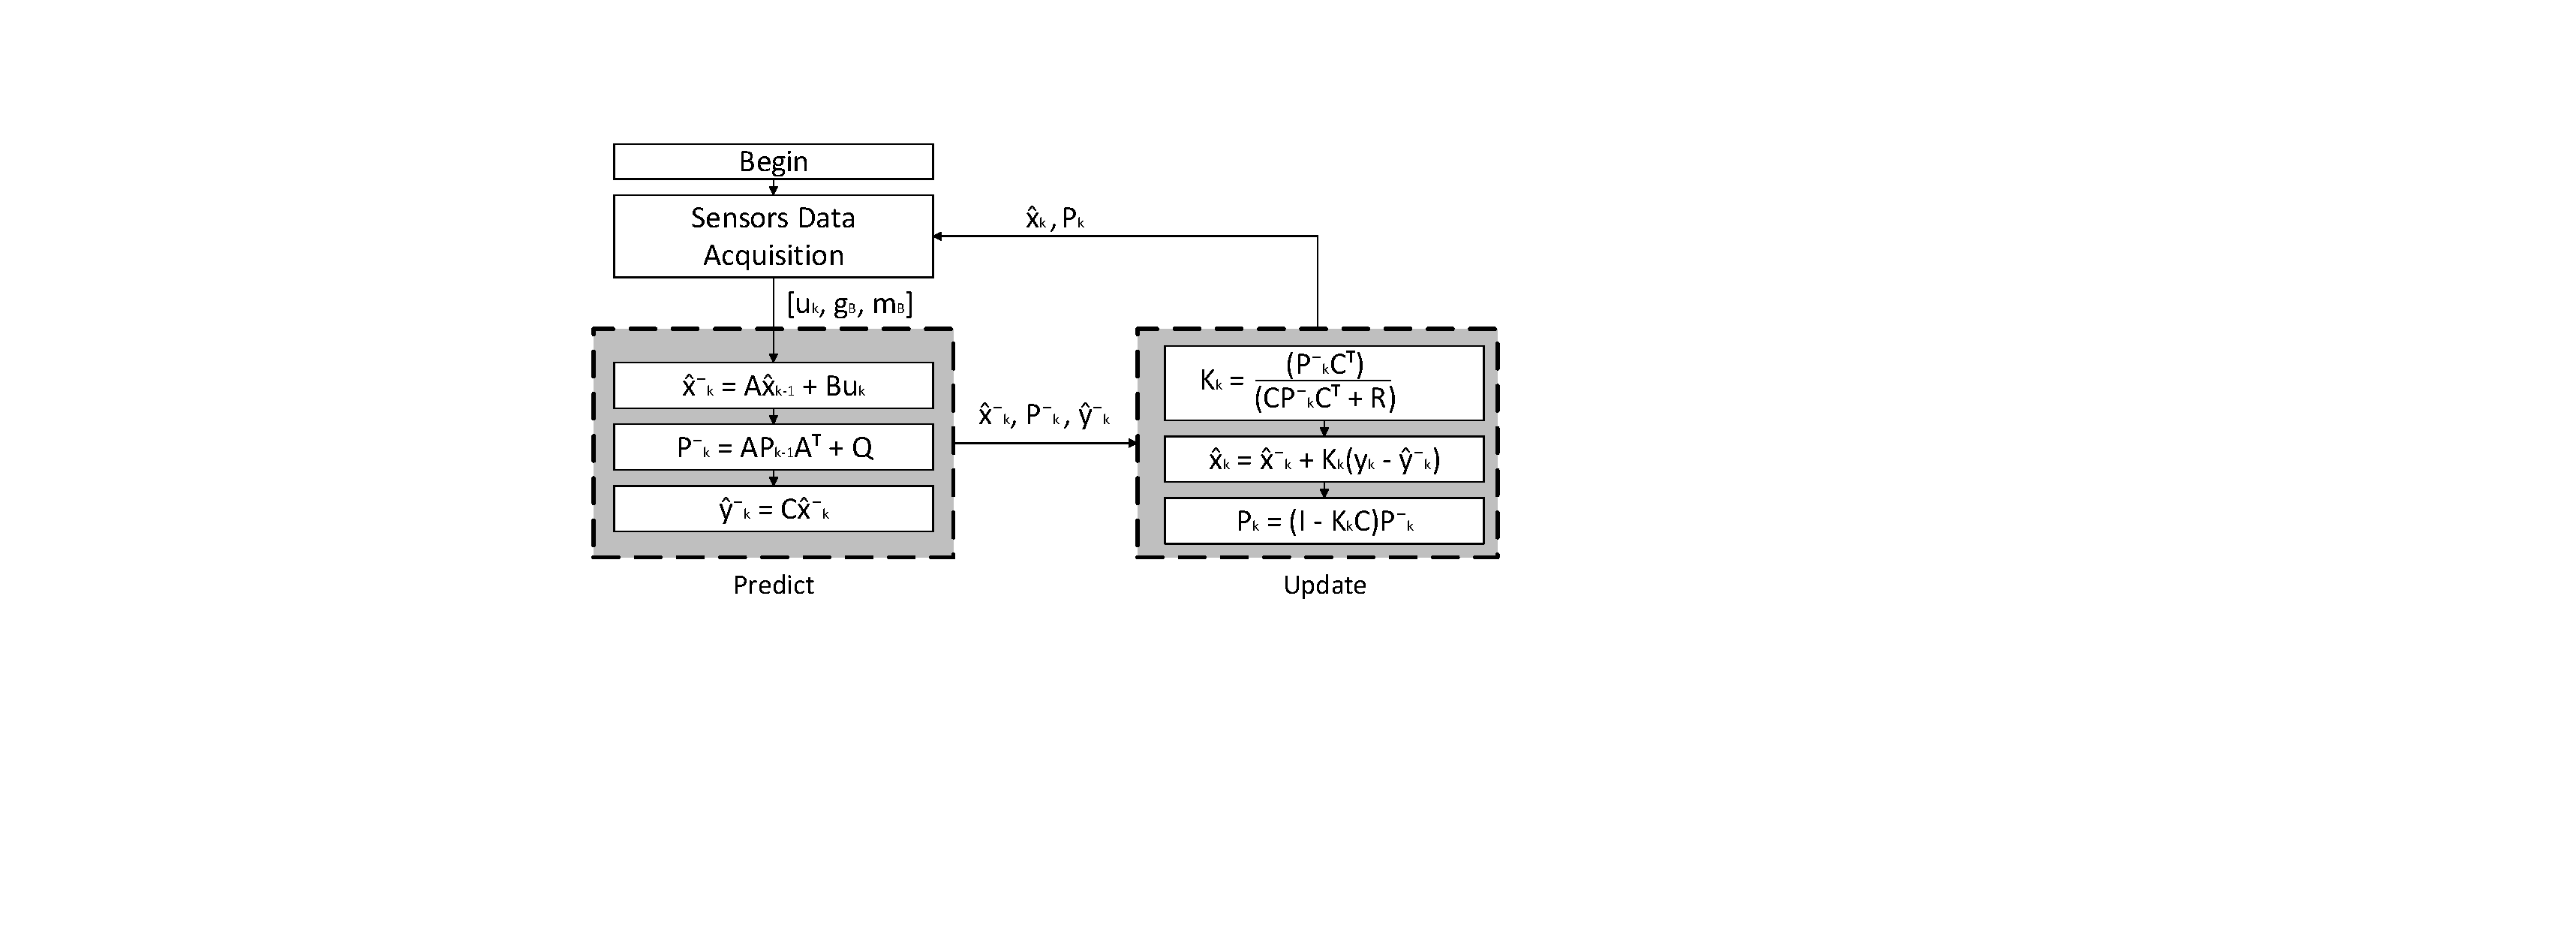
\includegraphics[width=0.5\linewidth]{UCSP_Pictures/imagen22.pdf}
    \caption{EKF process diagram.}
    \label{fig:ekf_processs}
    \end{figure}


    \item \textbf{Uncented Kalman Filter (UKF):} This filter estimates ($\mathbf{q}$) while managing its uncertainty with an error covariance matrix ($\mathbf{P} \in \Re^{3\times3}$). This matrix corresponds to a 3D rotation error vector, defined using an axis-angle representation as ($\boldsymbol{\delta\theta} = \vartheta \mathbf{e}$), where $\vartheta$ is the error angle and $\mathbf{e}$ is the associated unit axis of rotation. The high-frequency Predict step propagates a cloud of sigma points ($\chi_i$) through the kinematic model \eqref{eq_Kinematics_equation} using $\boldsymbol{\tilde{\omega}}_{meas}$ to forecast the new orientation. Subsequently, the low-frequency Correct step refines this forecast by transforming the sigma points into the measurement space using the model $\mathbf{y=R(q)^T v_{ref}}$ to predict $\tilde{\mathbf{f}}_{\text{meas}}$, $\tilde{\mathbf{m}}_{\text{meas}}$, and, optionally, $\mathbf{\tilde{s}}_{\text{meas},n}$. Based on the innovation, the difference between the actual and predicted measurements, it computes the Kalman gain ($\mathbf{K}$). It applies a multiplicative correction to the state, which robustly adjusts the orientation and reduces the error covariance.
\end{itemize}

\subsubsection{Phase 4: SAT-ABC Pointing mode}

In Phase 4, it is required to align SAT-ABC $Z_B$ axis with the translational velocity vector. For this purpose  two non-linear attitude control algorithms based on quaternions were evaluated, assuming that $\delta \mathbf{q}$ represents the quaternion error and $\delta \boldsymbol{\omega}$ the angular velocity error. It is important to note that the following descriptions assume that the torques are produced by internal torques from the reaction wheels, which oppose the external torque applied to the CubeSat, as provided by magnetorquers.

\begin{itemize}
    \item \textbf{Quaternion Feedback Controller}
\label{subsec_quatcontroller}
The tracking problem is defined by the error variables `$\delta\omega$' and `$\delta \beta $' defined in (\ref{qe_beta}).
\begin{equation}
\label{qe_beta}
   \delta \beta = q_{13}-q_{d 13}
\end{equation}

The control law is defined in (\ref{eq_controllaw}).
\begin{multline}
\label{eq_controllaw}
    u=P\delta\omega+K\delta\beta-[\omega\times](J_B\omega-J_{rw}(\omega+\Omega))
    -J_B(\dot{\omega}_d-[\omega\times]\omega_d)
\end{multline}

Where `K' and `P' are positive definite matrices, $\Omega$ are the reaction wheel angular rates, and $J_{rw}$ are the reaction wheel inertia values in the spin axes. 

\item \textbf{Boskovic Robust Controller:}
\label{subsec_Bosk}
 Boskovic's work \cite {Boskovic2004} is based on the variable-structure approach, and his control technique does not require prior knowledge of the inertia tensor. In addition, Boskovic designed an adaptive gain that allows for compensating the disturbance torques and ensures that attitude and angular velocity errors will tend to zero.

The control law proposed by Boskovic is given by (\ref{Eq_Boskoviccontrol}).
\begin{equation}
\label{Eq_Boskoviccontrol}
    -u_i(t)=-u_{max}\frac{s_i(t)}{|s_i(t)|+k^2(t)\delta_k} \hspace{1cm} i=1,2,3
\end{equation}
Where `$\delta_k$' is a positive constant,  `K(t)' is the adaptive gain and  `$u_{max}$' is the torque limit for all control torques.
The Boskovic    Sliding Vector  `$s(t)$' is defined by (\ref{Eq_Boskovicslidingv}).
\begin{equation}
\label{Eq_Boskovicslidingv}
    s(t)=\delta\omega(t)+k^2\delta q_{13}(t)
\end{equation}
Boskovic defined, in \cite{Boskovic2004}, the adjustment law for the time-varying control gain as (\ref{eq_adap_gain}).
\begin{multline}
    \label{eq_adap_gain}
    \dot{k}(t)=\frac{\gamma k(t)}{1+4\gamma[1-\delta q_4(t)]}\left\{ u_{max} \sum_{i=1}^3\left[\frac{\delta\omega_i\delta q_i(t)}{|s_i(t)|+k^2(t)\delta_k}-\right.\right.\\
    \left.\left.\frac{|\delta \omega_i(t)|(1+\delta_k)}{|\delta\omega_i(t)|+k^2(t)(1+\delta_k)}\right]-\delta\omega^T\delta q_{13}-k^2\delta q_{13}^T\delta q_{13}\right\}
\end{multline}
where  `$\gamma$' is a positive scalar and is called the convergence rate.
\end{itemize}

Using the Quaternion Feedback Controller of (\ref{eq_controllaw}), the simulation results in the inertial frame are shown in Figures \ref{fig:attitude_quaternions}, \ref{fig:quaternion_error}, and \ref{fig:required_torque}, skipping the detumbling state, aligning to the translational velocity vector, and assuming unitary gains. As can be seen, the quaternion error remains around 0.3 degrees. However, an accurate knowledge of the inertia tensor is required.

\begin{figure}
    \centering
    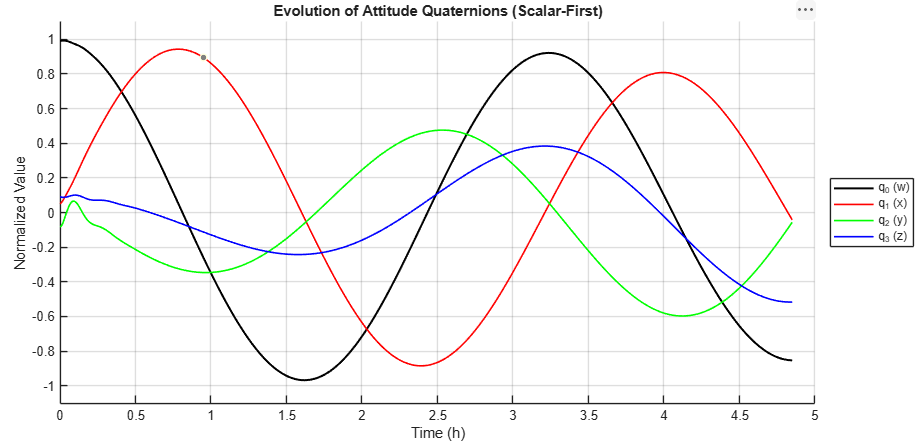
\includegraphics[width=0.8\linewidth]{UCSP_Pictures/SAT-ABC_Attitude_quaternions.png}
    \caption{SAT-ABC attitude quaternion using the Quaternion Feedback Controller of Eq. (\ref{eq_controllaw})}
    \label{fig:attitude_quaternions}
\end{figure}

\begin{figure}
    \centering
    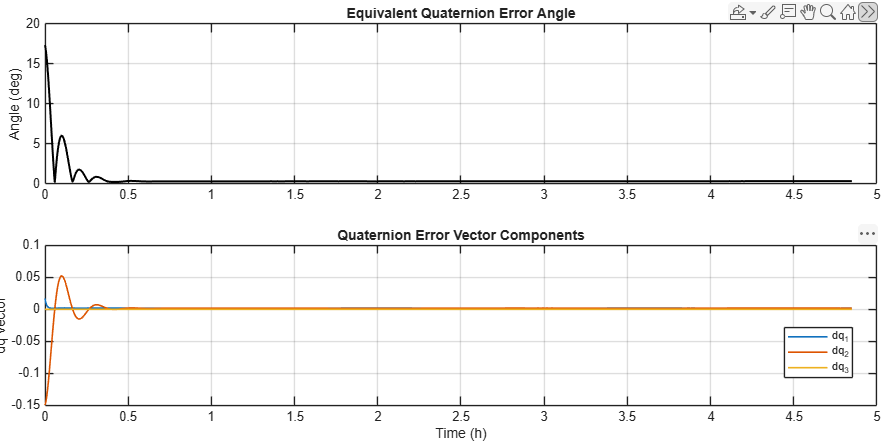
\includegraphics[width=0.8\linewidth]{UCSP_Pictures/SAT-ABC_Attitude_quaternions_error.png}
    \caption{SAT-ABC quaternion error or Euler angle error equivalent using the Quaternion Feedback Controller of Eq. (\ref{eq_controllaw}).}
    \label{fig:quaternion_error}
\end{figure}

\begin{figure}
    \centering
    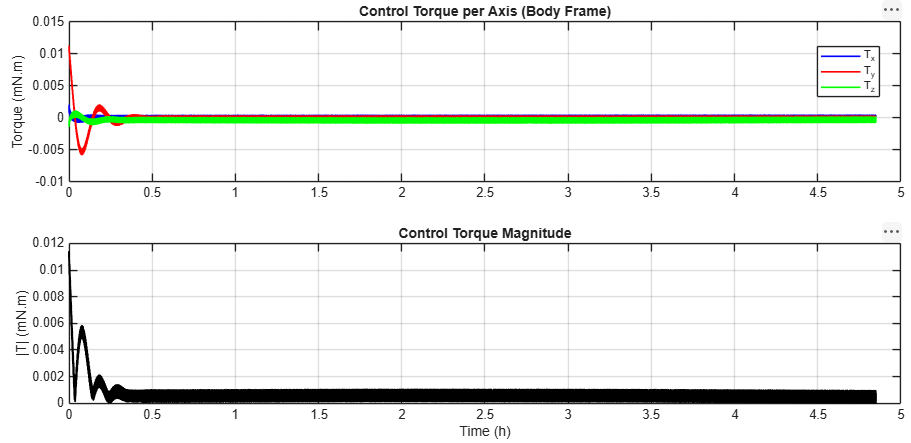
\includegraphics[width=0.8\linewidth]{UCSP_Pictures/SAT-ABC_triaxial_Torque.png}
    \caption{SAT-ABC control torque calculated with the Quaternion Feedback Controller of Eq. (\ref{eq_controllaw})}
    \label{fig:required_torque}
\end{figure}


Since the satellite's inertia tensor is difficult to measure precisely, the adaptive controller developed by Boskovic et al. \cite{Boskovic2004} was evaluated. Figures \ref{fig:attitude_quaternions_bosk}, \ref{fig:quaternion_error_bosk}, and \ref{fig:required_torque_bosk} present the SAT-ABC attitude quaternions aligned with the velocity vector, the quaternion error alongside the equivalent Euler angle, and the control torque, respectively. As illustrated, this controller outperforms the conventional quaternion controller when there is no prior knowledge of the satellite's inertia tensor, achieving asymptotic convergence to the desired target point under the assumption of ideal actuators.

\begin{figure}
    \centering
    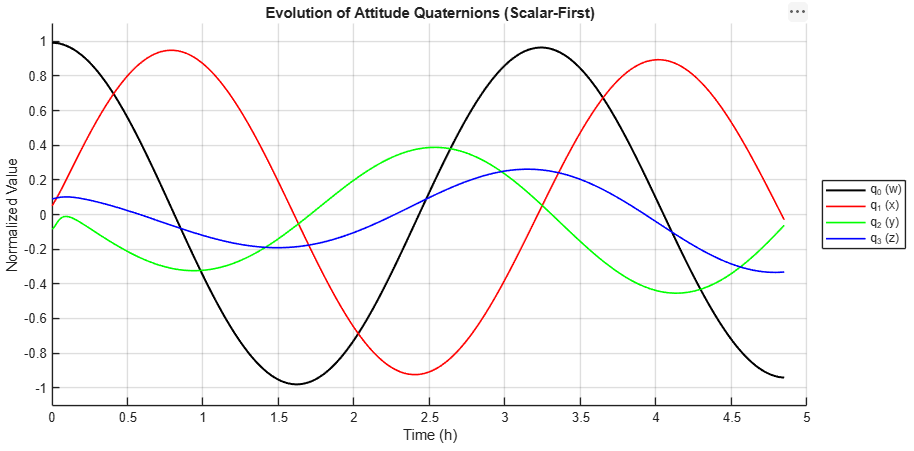
\includegraphics[width=0.8\linewidth]{UCSP_Pictures/SAT-ABC_Attitude_quaternions_bosk.png}
    \caption{SAT-ABC attitude quaternion using the Boskovic of \cite {Boskovic2004}}
    \label{fig:attitude_quaternions_bosk}
\end{figure}

\begin{figure}
    \centering
    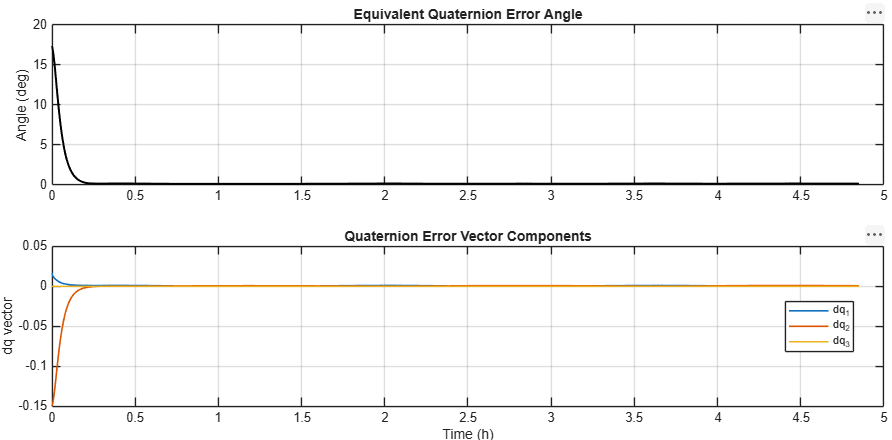
\includegraphics[width=0.8\linewidth]{UCSP_Pictures/SAT-ABC_Attitude_quaternions_error_bosk.png}
    \caption{SAT-ABC quaternion error or Euler angle error equivalent using the Boskovic \cite {Boskovic2004}.}
    \label{fig:quaternion_error_bosk}
\end{figure}

\begin{figure}
    \centering
    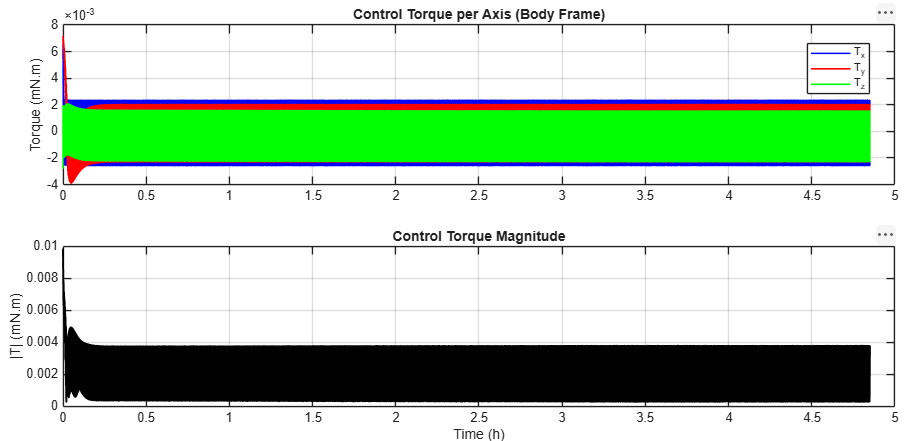
\includegraphics[width=0.8\linewidth]{UCSP_Pictures/SAT-ABC_triaxial_Torque_bosk.png}
    \caption{SAT-ABC control torque calculated with tthe Boskovic \cite {Boskovic2004}.}
    \label{fig:required_torque_bosk}
\end{figure}



%\subsubsection{Phase 5: Deployment of SAT-BC}
%After the deployment of SAT-BC, the satellite SAT-A remains alone.


\subsection{Stage II: Dynamics of the Coupled SAT-BC}
\textbf{Phase 6:} Body SAT-BC  released from SAT-ABC
\begin{itemize}
    \item \textbf{Power-On Self-Test (POST):} The system verifies the electrical and structural integrity of the ADCS sensors and actuators to ensure no damage was sustained.
    \item \textbf{Sensor Calibration and Biasing:} Biasing and noise characterization are performed during the initial free-drift state. The gyroscopes and magnetometers are calibrated using Extended Kalman Filters (EKF) and sphere-fitting algorithms to identify constant biases and hard-iron displacements, ensuring high-fidelity attitude estimation.
    \item \textbf{Reference Frame Synchronization and Parameter Identification:} The SAT-BC geometric axes are mapped within the flight software. Similarly to Phase 1, this step involves a passive estimation of the inertia tensor and Center of Mass.
    \item \textbf{Initial Attitude Determination:} A coarse orientation is resolved by implementing the TRIAD algorithm, which processes solar and magnetic field vectors to establish a stable baseline attitude before initiating the Phase 2 detumbling maneuver.
\end{itemize}

\textbf{Phase 7:} Body SAT-BC gradually reduces its rotation rate (detumbling) and subsequently achieves a detumbling stabilization using an ADCS composed solely of magnetorquers. For testing purposes, the inertia tensor calculated using Monte Carlo analysis in Table \ref{tab:monte_carlo_results} and the values presented in Table \ref{tab:SAT-BC_system_parameters} are used.

\begin{table}[htbp]
\centering
\caption{Technical Parameters for SAT-BC simulations}
\label{tab:SAT-BC_system_parameters}
\begin{tabular}{lll}
\toprule
\textbf{Parameter / Component} & \textbf{Value} & \textbf{Units} \\
%\midrule
%\textbf{Satellite} & & \\
%Mass ($m$) & 5.5 & kg \\
%Inertia Tensor ($I_s$) & $\begin{bmatrix} 0.0577 & 0.0010 & 0.0010 \\ 0.0010 & 0.5777 & -0.0020 \\ 0.0010 & -0.0020 & 0.0444 \end{bmatrix}$ & kg$\cdot$m$^2$ \\
\midrule
\rowcolor[HTML]{EFEFEF}
\textbf{Actuators: Magnetorquers} & & \\
Nominal / Maximum Power ($P$) & 0.360 & W \\
Voltage ($V$) & 5.0 & V \\
Dimensions ($w, h, l$) & $30 \times 30 \times 30$ & mm \\
Nominal / Maximum Dipole & 0.1 & A$\cdot$m$^2$ \\
Residual Dipole ($\mathbf{m}_{res}$) & $[0.004; -0.002; 0.003]^T$ & A$\cdot$m$^2$ \\
Linearity Factor (B-H curve) & 2.0 & --- \\
\midrule
\rowcolor[HTML]{EFEFEF} 
\textbf{Sensors: Magnetometer} & & \\
Noise Standard Deviation ($\sigma_{mag}$) & $150.00 \times 10^{-9}$ & T \\
Resolution & $10.00 \times 10^{-9}$ & T \\
Standard Deviation Norm & 0.5 & --- \\
Filter Time Constant ($\tau$) & 0.5 & s \\
\midrule
\rowcolor[HTML]{EFEFEF} 
\textbf{Sensors: Gyroscope (IMU)} & & \\
Scale Factor & $[0.005; 0.005; 0.005]^T$ & --- \\
Misalignment Matrix ($M_{mis}$) & $\begin{bmatrix} 0 & 0.001 & 0.001 \\ 0.001 & 0 & 0.001 \\ 0.001 & 0.001 & 0 \end{bmatrix}$ & rad \\
White Noise ($\eta_g$) & 0.05 & deg/s \\
Bias Instability ($\sigma_{RW}$) & 0.005 & deg/s/$\sqrt{\text{s}}$ \\
Filter Time Constant ($\tau$) & 0.1 & s \\
Saturation Limits ($y_{min}, y_{max}$) & $\pm 250$ & deg/s \\
ADC Resolution & 16 & bits \\
Reference Voltage ($V_{ref}$) & 3.3 & V \\
\bottomrule
\end{tabular}
\end{table}

The results of the montecarlo analisys and the statistical distribution of the settling times are depicted in Figure \ref{fig:monte_carlo_results_SAT-BC}. 

\begin{itemize}
    \item \textbf{Convergence Rate:} A 100\% success rate was achieved, with 50 out of 50 runs reaching the stabilization threshold ($< 1.00$ deg/s).
    \item \textbf{First Crossing Time:} The initial crossing of the threshold occurs at a mean time of \textbf{1.55 h}. The distribution in the ``First crossings'' histogram highlights the varying convergence behaviors depending on the initial kinetic energy and the orbital magnetic field alignment.
    \item \textbf{Verified Detumbling Time:} To ensure stability, a mandatory Hold-time of 3600 s (1.00 h) was implemented. The ``Verified runs'' analysis shows that the satellite achieves a fully verified stable state within a mean time of 2.55 h, with a best-case (minimum) time of 0.2h and a worst-case scenario (maximum time) of 4.76 h.
    \item \textbf{Robustness against Resets:} The ``Hold-time and reset effect'' histogram validates that the verification delay remains tightly grouped around the 1.00 h mark (with a mean delay of 1.00 h). This confirms that the hysteresis logic (Reset threshold at 1.20 deg/s) effectively prevents premature transitions due to sensor noise or residual dipoles.
\end{itemize}

The results demonstrate that the SAT-BC will achieve a stable state within approximately 1.6 to 3 orbits (considering a $\sim$96 min orbit), providing a reliable baseline for subsequent operational phases such as nominal alignment.

\begin{figure}
    \centering
    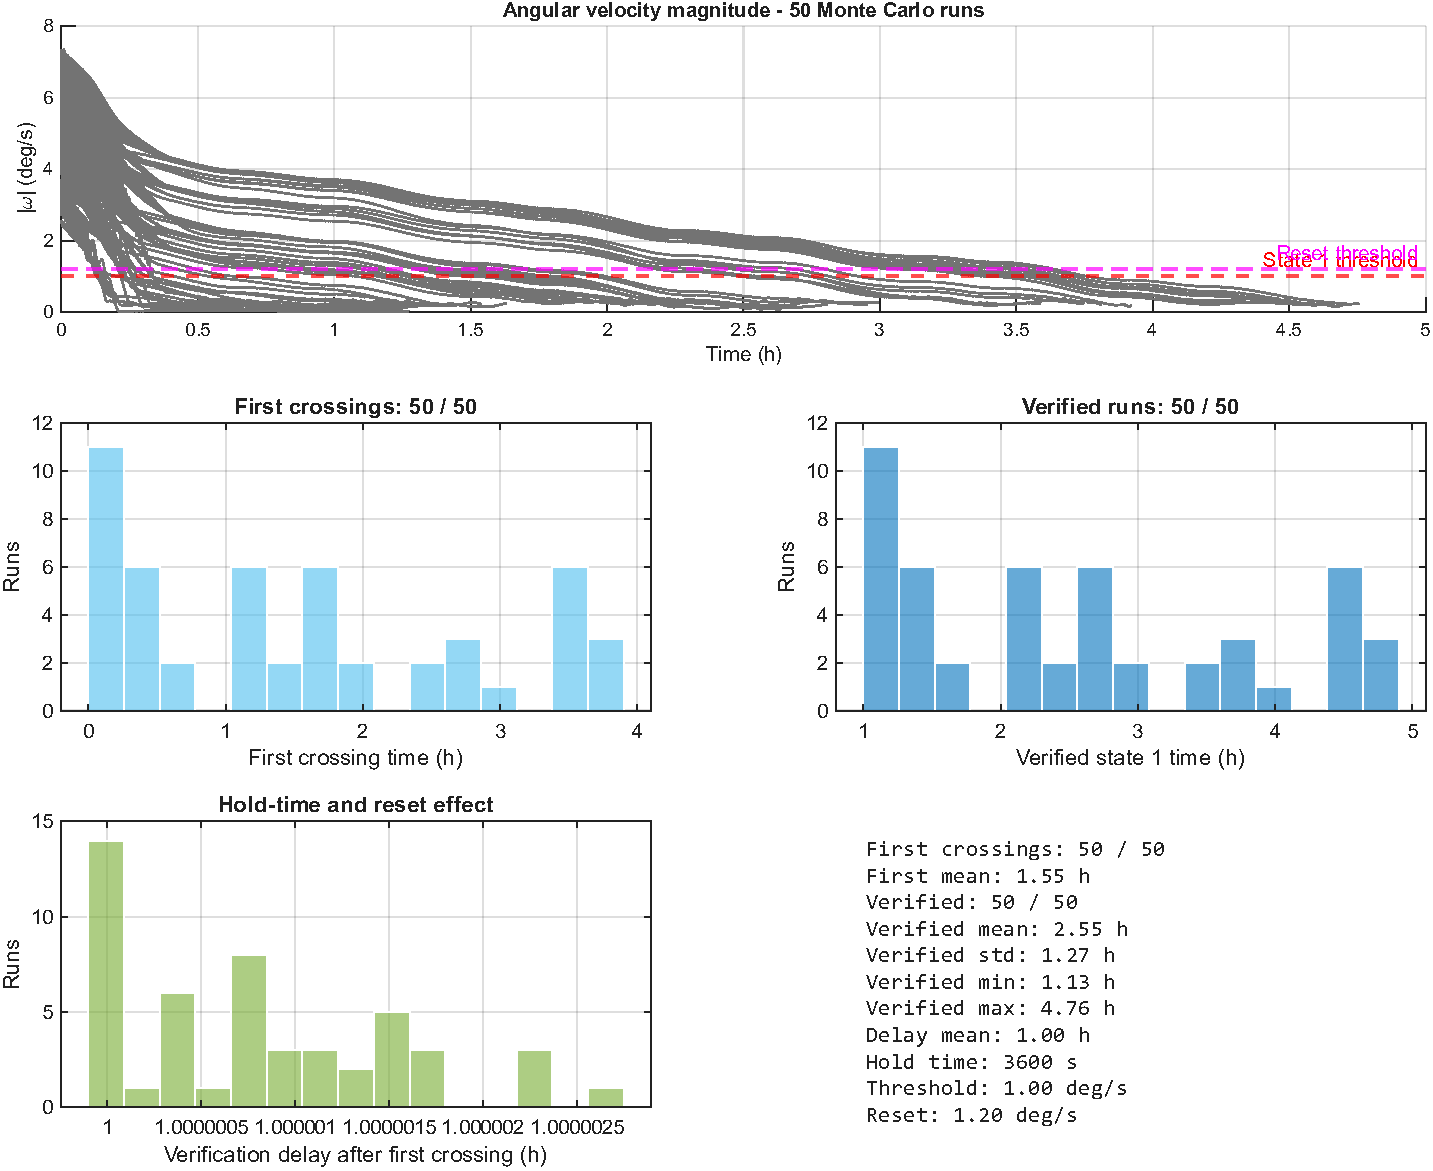
\includegraphics[width=0.9\linewidth]{UCSP_Pictures/State 1 Verification_SAT-BC.pdf}
    \caption{Monte Carlo simulation results for the detumbling phase of SAT-ABC: angular velocity convergence and settling time distributions.}
    \label{fig:monte_carlo_results_SAT-BC}
\end{figure}
%\subsection{Hardware Configuration}

\subsubsection{Phase 9:  SAT-BC pointing Mode}
Since the ADCS study for SAT-ABC is based on the iADCS400 module, it is necessary to perform a state of the art review to propose an ADCS for the SAT-BC body pointing mode. Table \ref{tab:state_of_the_art} summarizes the main characteristics of some 1U to 3U small satellite missions. This comparison aims to characterize the performance of purely magnetic actuators and the significant reliance on the B-dot law during the initial stabilization phase in satellites with mass properties similar to SAT-BC.

\begin{table}[h]
    \centering
    \caption{Comparison of 1U to 3U missions and its ADCS strategies.}
    \label{tab:state_of_the_art}
    \renewcommand{\arraystretch}{1.5} 
    \footnotesize 
    % Se definen anchos fijos para que sumen el ancho de página aproximado
    \begin{tabular}{|p{3.2cm}|p{2.0cm}|p{2.0cm}|p{3.1cm}|p{3.1cm}|}
        \hline
        %\rowcolor{gray!20}
        \rowcolor[HTML]{EFEFEF}
        \textbf{Mission / Study} & \textbf{Mass} & \textbf{Actuators} & \textbf{Detumbling Algorithm} & \textbf{Achieved Accuracy} \\ \hline
        
        A Fully Magnetic Approach to ADCS \cite{bono2024fully} & Nanosatellites & Magnetorquers only (fully magnetic system). & Evaluates and compares two strategies: Classic B-dot law and Model Predictive Control (MPC). & Less than 20$^\circ$ (magnetometer only). Less than 3$^\circ$ (fusing data with gyroscopes). \\ \hline
        
        MPC-Based Magnetorquer Control \cite{esit2022model} & Microsatellites (5-10 kg) in LEO Sun-synchronous orbit. & Magnetorquers only (3 orthogonal coils). & Magnetorquers are the primary method to dissipate initial kinetic energy. & Convergence with residual errors $< 5^\circ$ in steady state (MPC outperforms traditional LQR). \\ \hline
        
        ODIN Nano-Satellite \cite{odin_project} & 3U CubeSat ($\approx 4$ kg). & Magnetorquers for attitude control and desaturation. & Initial stabilization to achieve pointing of UV sensors toward the atmosphere. & Maintains necessary orientation to perform UV photometry of the ozone layer. \\ \hline
        
        ST3LLARsat1 "BOIRA" \cite{marcos2023st3llarsat1} & 2U CubeSat. & 3 Magnetorquers only. & Divided into two strict phases: Detumbling and Attitude Pointing. & Attitude knowledge error: 3$^\circ$. Pointing error: 5$^\circ$. \\ \hline
        
        E.T.PACK / Deorbit Kit \cite{garciagonzalez2023avionic} & Nano and microsatellites (dockable module). & Intensive use of magnetorquers and electromagnetic interaction analysis. & Implements and analyzes B-dot controller robustness against external forces generated by the tether. & High robustness against external deorbiting perturbations. \\ \hline
        
        Magnetic ADCS for Picosatellites \cite{giesselmann2024development} & Nano and microsatellites. & 3 Magnetorquers only. & B-dot controller (used to stabilize the satellite before transitioning to advanced predictive control). & Pointing error $< 5^\circ$. \\ \hline
        
    \end{tabular}
\end{table}

While satellites relying exclusively on magnetic actuators and robust controllers (e.g., MPC) typically achieve a nadir-pointing accuracy of roughly 5°, preliminary simulations of the SAT-ABC algorithms exhibited Euler angle errors reaching 120°. To address this limitation and enhance both pointing accuracy and system reliability, future work will transition to a hybrid actuation system integrating an orthogonal triad of magnetorquers with a reaction wheel.

%As can be observed, most satellites relying solely on magnetic actuators achieve a nadir-pointing accuracy of approximately 5 degrees when employing robust controllers such as MPC and preliminary results using the algorithms presented for SAT-ABC shows Euler angle error up to 120 degrees which is unaceptable. Therefore, to enhance pointing performance and system reliability, future work will focus on implementing a hybrid configuration that combines an orthogonal triad of magnetorquers with a reaction wheel.
\end{comment}


\newpage
\section{Attitude Determination and Control System}
\label{sec:adcs}

\subsection{Scope and Operational Role of the ADCS}
\label{sub:adcs_scope_operational_role}

The Attitude Determination and Control System (ADCS) supports the attitude stabilization and pointing functions required for the LINKU tether deployment experiment. The ADCS analysis in this section follows the mission stages and steps defined in Section~\ref{sec:mission_conops}, with emphasis on the active attitude-control functions required before SAT-B/SAT-C separation.

During Mission Stage~1, the ADCS is responsible for the initial detumbling, stabilization, attitude-determination convergence, and deployment orientation of the SAT-ABC configuration. These functions correspond mainly to Steps~1.2--1.4, where the integrated spacecraft must reduce its angular rate, verify attitude-estimation convergence, and orient itself to RAM direction for the release of SAT-BC.

During Mission Stage~2, the ADCS supports the detumbling, stabilization, attitude-determination convergence, and nadir-pointing preparation of the SAT-BC configuration. These functions correspond mainly to Steps~2.2--2.4, where the coupled SAT-B/SAT-C body must reach a stable attitude condition and align itself to NADIR direction before the SAT-B/SAT-C separation command.

After SAT-B/SAT-C separation, the tethered system transitions to passive gravity-gradient behavior, as defined in Mission Stage~3. Therefore, the ADCS analysis presented in this section focuses on the active pre-separation configurations, SAT-ABC and SAT-BC. SAT-A post-deployment re-stabilization and secondary mission operations are acknowledged as part of Mission Stage~4, but their detailed ADCS design is outside the scope of the present analysis.

\subsection{ADCS Modeling Methodology}
\label{sub:adcs_modeling_methodology}
The preliminary ADCS assessment is based on a simulation framework that combines rigid-body attitude dynamics, orbital propagation, environmental disturbance models, sensor and actuator models, and control algorithms. This framework is used to evaluate the feasibility of the active attitude-control functions required for the SAT-ABC and SAT-BC configurations before SAT-B/SAT-C separation.

The methodology includes the definition of the satellite reference frames, kinematic and dynamic equations, the estimation of mass properties and inertia uncertainty, the modeling of the orbital, geomagnetic, and disturbance environment, and the implementation of representative sensor and actuator models. The main body of this section presents the models, parameters, and results needed to support the preliminary ADCS assessment. More detailed implementation aspects, including full sensor-error models, ADC quantization, extended attitude-estimation algorithm descriptions, actuator internal models, and supplementary orbital-environment results, are provided in Appendix~\ref{app:adcs_detailed_models}.

\subsubsection{LINKU Reference Frames}
\label{subsub:reference_frames}

The body-fixed reference frames used for the SAT-ABC and SAT-BC simulations are shown in Figure~\ref{fig:adcs_satellite_body_frames}. The origin of each body frame is located at the corresponding center of mass. The inertial reference frame used in the simulations is the Geocentric Celestial Reference Frame (GCRF). The orbital reference frame follows the LVLH convention adopted in Deliverable~D4, where the \(Z\)-axis points toward nadir and the \(X\)-axis is aligned with the satellite velocity vector.

\begin{figure}[htbp]
    \centering
    \begin{subfigure}[b]{0.48\textwidth}
        \centering
        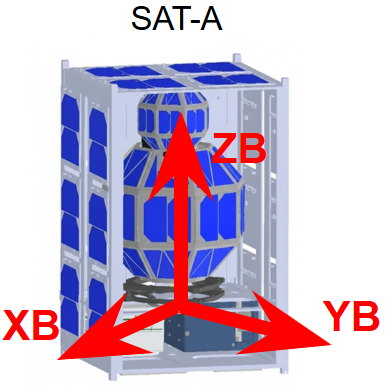
\includegraphics[height=6cm,keepaspectratio
        ]{UCSP_Pictures/sat_abc_body_frame.png}
        \caption{}
        \label{fig:adcs_satabc_body_frame}
    \end{subfigure}
    \hfill
    \begin{subfigure}[b]{0.48\textwidth}
        \centering
        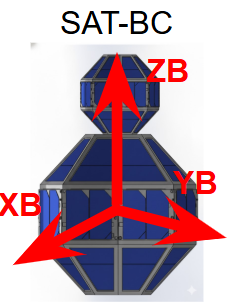
\includegraphics[height=6cm,keepaspectratio
        ]{UCSP_Pictures/sat_bc_body_frame.png}
        \caption{}
        \label{fig:adcs_satbc_body_frame}
    \end{subfigure}
    \caption{Body-fixed reference frames used for the ADCS analysis:
    (a) SAT-ABC body-fixed reference frame;
    (b) SAT-BC body-fixed reference frame.}
    \label{fig:adcs_satellite_body_frames}
\end{figure}

\subsubsection{Satellite Kinematics and Dynamics}
\label{subsub:adcs_kinematics_dynamics}

The satellite attitude is represented using the quaternion notation
\(\mathbf{q} = [q_0, q_1, q_2, q_3]^T\), where \(q_0\) is the scalar component and \(q_1\), \(q_2\), and \(q_3\) are the vector components. The quaternion kinematic equation is given by \eqref{eq:adcs_quaternion_kinematics}~\cite{crassidis2021spacecraft}.

\begin{equation}
    \dot{\mathbf{q}} = \frac{1}{2}\mathbf{\Xi}(\mathbf{q})\boldsymbol{\omega},
    \label{eq:adcs_quaternion_kinematics}
\end{equation}

where \(\boldsymbol{\omega} \in \mathbb{R}^{3}\) is the satellite angular rate relative to the inertial frame expressed in the body frame, and \(\mathbf{\Xi}(\mathbf{q})\) is defined as \eqref{eq:adcs_xi_matrix}.

\begin{equation}
    \mathbf{\Xi}(\mathbf{q}) =
    \begin{bmatrix}
        -q_1 & -q_2 & -q_3 \\
         q_0 & -q_3 &  q_2 \\
         q_3 &  q_0 & -q_1 \\
        -q_2 &  q_1 &  q_0
    \end{bmatrix}.
    \label{eq:adcs_xi_matrix}
\end{equation}

The rotational dynamics are modeled using Euler's rigid-body equation, including control torques, environmental disturbance torques, and reaction-wheel angular momentum effects. The angular acceleration is expressed as \eqref{eq:adcs_rotational_dynamics}

\begin{equation}
    \dot{\boldsymbol{\omega}}
    =
    \mathbf{J}^{-1}
    \left[
        \mathbf{T}_{c}
        + \mathbf{T}_{d}
        - \dot{\mathbf{L}}_{\mathrm{rw}}
        - [\boldsymbol{\omega}\times]
        \left(
            \mathbf{J}\boldsymbol{\omega}
            + \mathbf{L}_{\mathrm{rw}}
        \right)
    \right],
    \label{eq:adcs_rotational_dynamics}
\end{equation}

where \(\mathbf{J} \in \mathbb{R}^{3\times3}\) is the satellite inertia tensor expressed in the body frame relative to the satellite center of mass, \(\mathbf{T}_{c} \in \mathbb{R}^{3}\) is the applied control torque, \(\mathbf{T}_{d} \in \mathbb{R}^{3}\) is the disturbance torque, and \(\mathbf{L}_{\mathrm{rw}} \in \mathbb{R}^{3}\) is the angular momentum of the reaction-wheel assembly expressed in the body frame. The operator \([\boldsymbol{\omega}\times]\) denotes the skew-symmetric matrix associated with the cross product.

\subsubsection{Mass Properties and Inertia Analysis}
\label{subsub:adcs_mass_properties}
The ADCS performance depends strongly on the mass properties of each satellite configuration, particularly the center of mass and inertia tensor. For this reason, a Monte Carlo analysis was performed to estimate the dispersion of the inertia tensor components under representative mass and assembly uncertainties. The analysis considered \(10{,}000\) samples and was applied to the SAT-ABC and SAT-BC configurations.

For the preliminary analysis, the satellite system was modeled as a multibody assembly composed of the SAT-A bus and the SAT-B/SAT-C payload elements. SAT-A was represented using a reference 12U CubeSat chassis geometry based on the EnduroSat 12U baseline. SAT-B was modeled as a hollow spherical-equivalent body with a mass of \(5~\mathrm{kg}\) and a radius of \(10~\mathrm{cm}\), while SAT-C was modeled as a smaller hollow spherical-equivalent body with a mass of \(0.5~\mathrm{kg}\) and a radius of \(5~\mathrm{cm}\).  Mass uncertainty, assembly tolerance, and nominal offsets of SAT-B and SAT-C were included to evaluate the sensitivity of the resulting inertia tensor as are summarized in Table~\ref{tab:adcs_inertia_properties}.

Additionally, the selected values presented in Table~\ref{tab:adcs_inertia_properties} correspond to conservative inertia cases derived from the Monte Carlo distributions, using the $+3\sigma$ threshold under a Gaussian approximation. These results serve as inputs for the subsequent control simulations.

\begin{table}[ht]
\centering
\caption{Representative mass and inertial properties for the SAT-ABC and SAT-BC configurations, including structural misalignments and mass uncertainties.}
\label{tab:adcs_inertia_properties}
\begin{tabular}{lcc}
\hline
\textbf{Parameter} & \textbf{SAT-ABC} & \textbf{SAT-BC} \\ \hline
Total mass (kg) & 8.8964 & 7.1500 \\
Center of mass (m) & $[0.0015, -0.0011, -0.0207]$ & $[0.0019, -0.0013, 0.0107]$ \\ \hline
\textbf{Uncertainties and misalignments} & \multicolumn{2}{c}{} \\ \hline
Mass uncertainty margin & \multicolumn{2}{c}{30.0\%} \\
Assembly tolerance ($3\sigma$) & \multicolumn{2}{c}{2.0 mm} \\
Nominal offset SAT-B (mm) & \multicolumn{2}{c}{$[2.0, -1.5, 0.0]$} \\
Nominal offset SAT-C (mm) & \multicolumn{2}{c}{$[-1.0, 2.0, 0.0]$} \\ \hline
\textbf{Inertia tensor, $\mathbf{J}_{\mathrm{CoM}}$} & \multicolumn{2}{c}{\textbf{Components [kg$\cdot$m$^2$]}} \\ \hline
$J_{xx}$ & 0.1339 & 0.0577 \\
$J_{yy}$ & 0.1341 & 0.0577 \\
$J_{zz}$ & 0.0704 & 0.0444 \\
$J_{xy}$ & -0.0000 & 0.0000 \\
$J_{xz}$ & -0.0003 & 0.0001 \\
$J_{yz}$ & -0.0001 & -0.0002 \\ \hline
\end{tabular}
\end{table}

Figure~\ref{fig:adcs_montecarlo_inertia_analysis} shows the Monte Carlo distributions obtained for the inertia-tensor components of the SAT-ABC and SAT-BC configurations. The statistical dispersion confirms that both configurations present small but non-negligible variations in their inertia properties due to mass uncertainty and assembly tolerances. These variations are relevant for the robustness assessment of the control algorithms and for the preliminary verification of actuator authority.

\begin{figure}[htbp]
    \centering
    \begin{subfigure}[b]{0.48\linewidth}
        \centering
        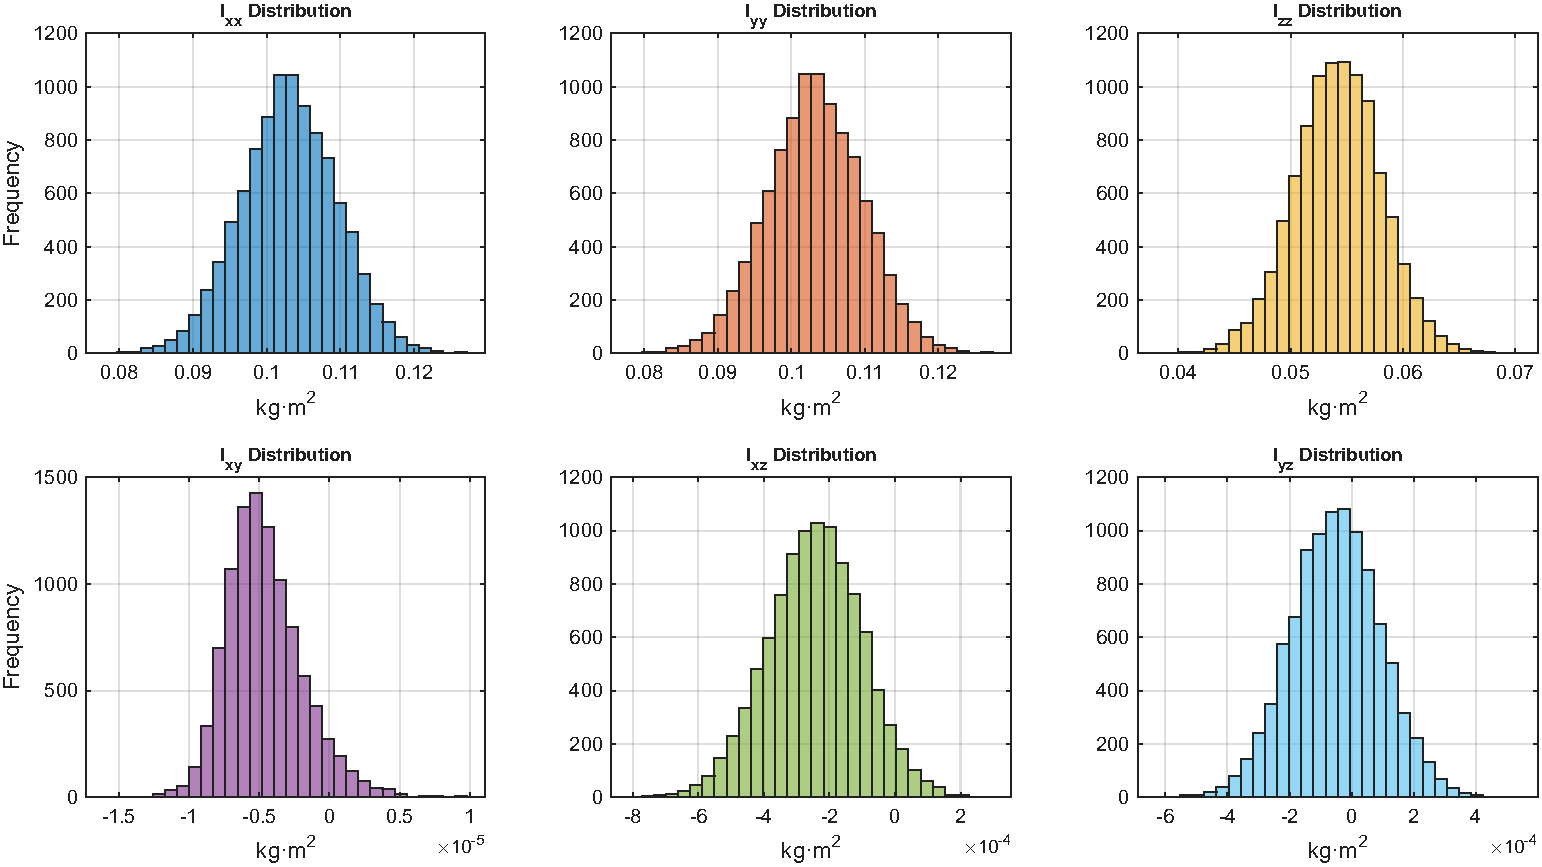
\includegraphics[width=\linewidth]{UCSP_Pictures/SAT-ABC.pdf}
        \caption{Monte Carlo analisys of the SAT-ABC Inertia tensor.}
        \label{fig:adcs_montecarlo_satabc}
    \end{subfigure}
    \hfill
    \begin{subfigure}[b]{0.48\linewidth}
        \centering
        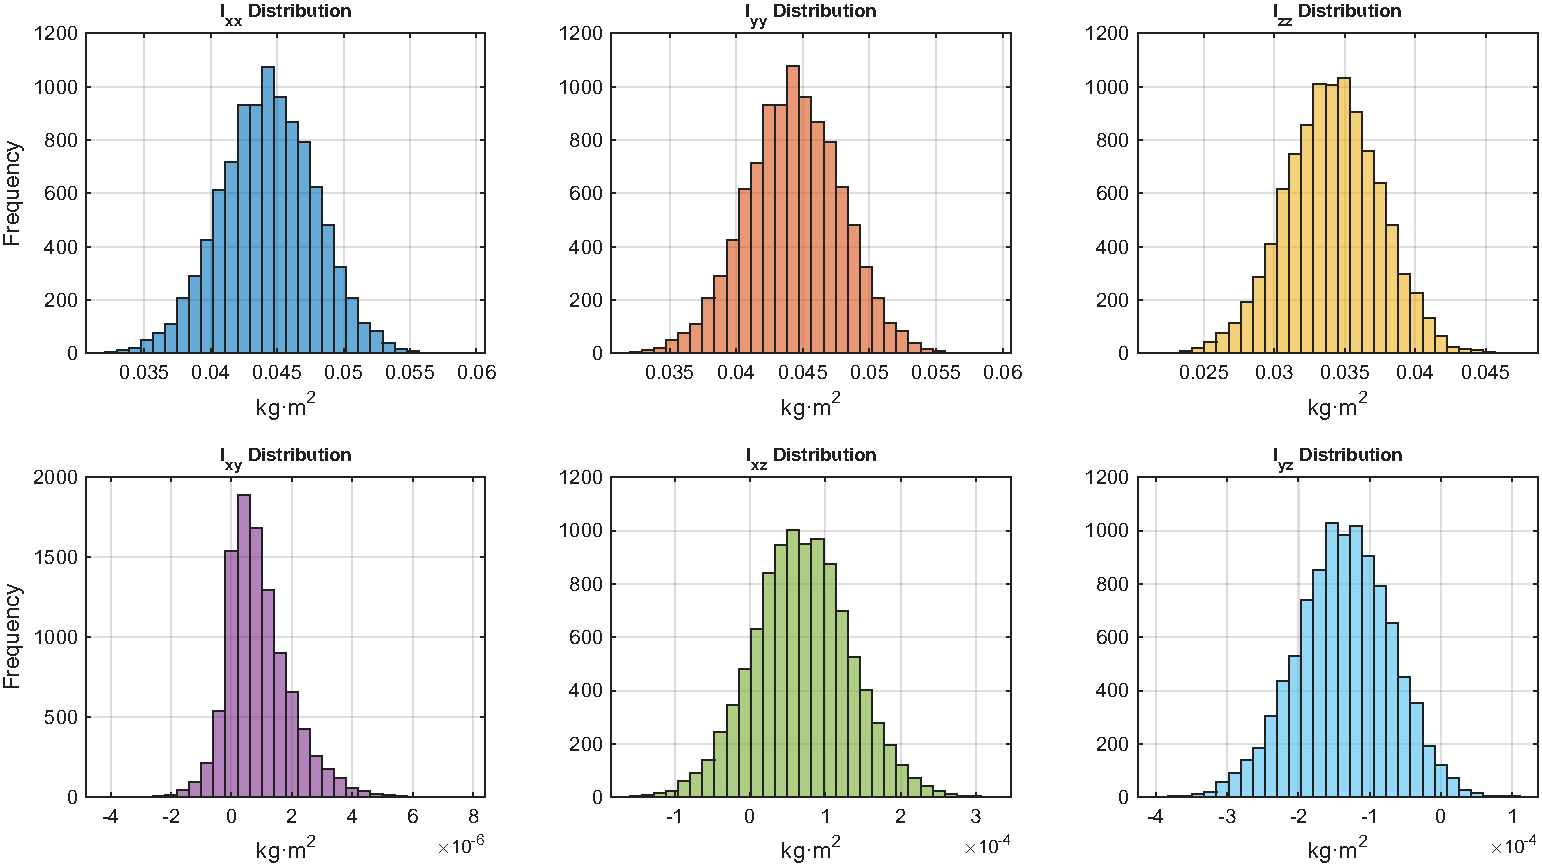
\includegraphics[width=\linewidth]{UCSP_Pictures/SAT-BC.pdf}
        \caption{Monte Carlo analisys of the SAT-BC Inertia tensor.}
        \label{fig:adcs_montecarlo_satbc}
    \end{subfigure}
    \caption{Monte Carlo analysis of the inertia-tensor components for the SAT-ABC and SAT-BC configurations.}
    \label{fig:adcs_montecarlo_inertia_analysis}
\end{figure}

The complete statistical results of the Monte Carlo analysis, including mean values, standard deviations, and minimum and maximum values for each inertia component, are provided in Appendix~\ref{app:adcs_detailed_models}.

\newpage
\subsubsection{Orbital, Geomagnetic, and Disturbance Environment}
\label{subsub:adcs_environment}

The ADCS simulations require an orbital and environmental model to compute the reference frames, geomagnetic field, and external disturbance torques acting on the satellite. For this purpose, satellite orbital propagation was performed using the Orekit suite, with a numerical propagator based on an adaptive variable-step Dormand--Prince 8(5,3) integrator. The model includes the Harris--Priester atmospheric drag model, third-body gravitational acceleration from the Sun and the Moon, and isotropic solar radiation pressure~\cite{maisonobe_2026_18527188}.

The orbital elements used for the ADCS simulations are summarized in Table~\ref{tab:adcs_orbit_params}. The same orbital propagation model is used for the SAT-ABC and SAT-BC configurations, since both operate in close orbital proximity during the active pre-separation stages of the LINKU mission.

\begin{table}[ht]
\centering
\caption{Orbital elements and mission environment used for the ADCS simulations.}
\label{tab:adcs_orbit_params}
\begin{tabular}{lll}
\toprule
\textbf{Orbital Element} & \textbf{Value} & \textbf{Unit} \\
\midrule
Semi-major axis, \(a\) & 6992000.0 & m \\
Eccentricity, \(e\) & 0.0037118 & -- \\
Inclination, \(i\) & 97.799 & deg \\
RAAN, \(\Omega\) & 80.477 & deg \\
Argument of perigee, \(\omega\) & 65.443 & deg \\
True anomaly, \(\nu\) & 294.6817 & deg \\
\midrule
Mean altitude, \(h\) & 613863.0 & m \\
Orbital period, \(T\) & 5818.5 & s \\
Circular velocity, \(v_c\) & 7550.5 & m/s \\
\bottomrule
\end{tabular}
\end{table}

The geomagnetic field is modeled using the International Geomagnetic Reference Field (IGRF). The IGRF coefficients are evaluated at the satellite position along the propagated orbit and transformed consistently with the reference frames used in the ADCS simulation. 

Figure~\ref{fig:adcs_orbital_environment_simulation} illustrates the LVLH orbital frame relative to the inertial frame, along with the resulting geomagnetic field simulation expressed in inertial coordinates. This field model is essential for the magnetorquer-based detumbling and stabilization analyses, as the control torque generated by the actuators directly depends on the local geomagnetic field vector.

\begin{figure}[htbp]
    \centering
    \begin{subfigure}[b]{\textwidth}
        \centering
        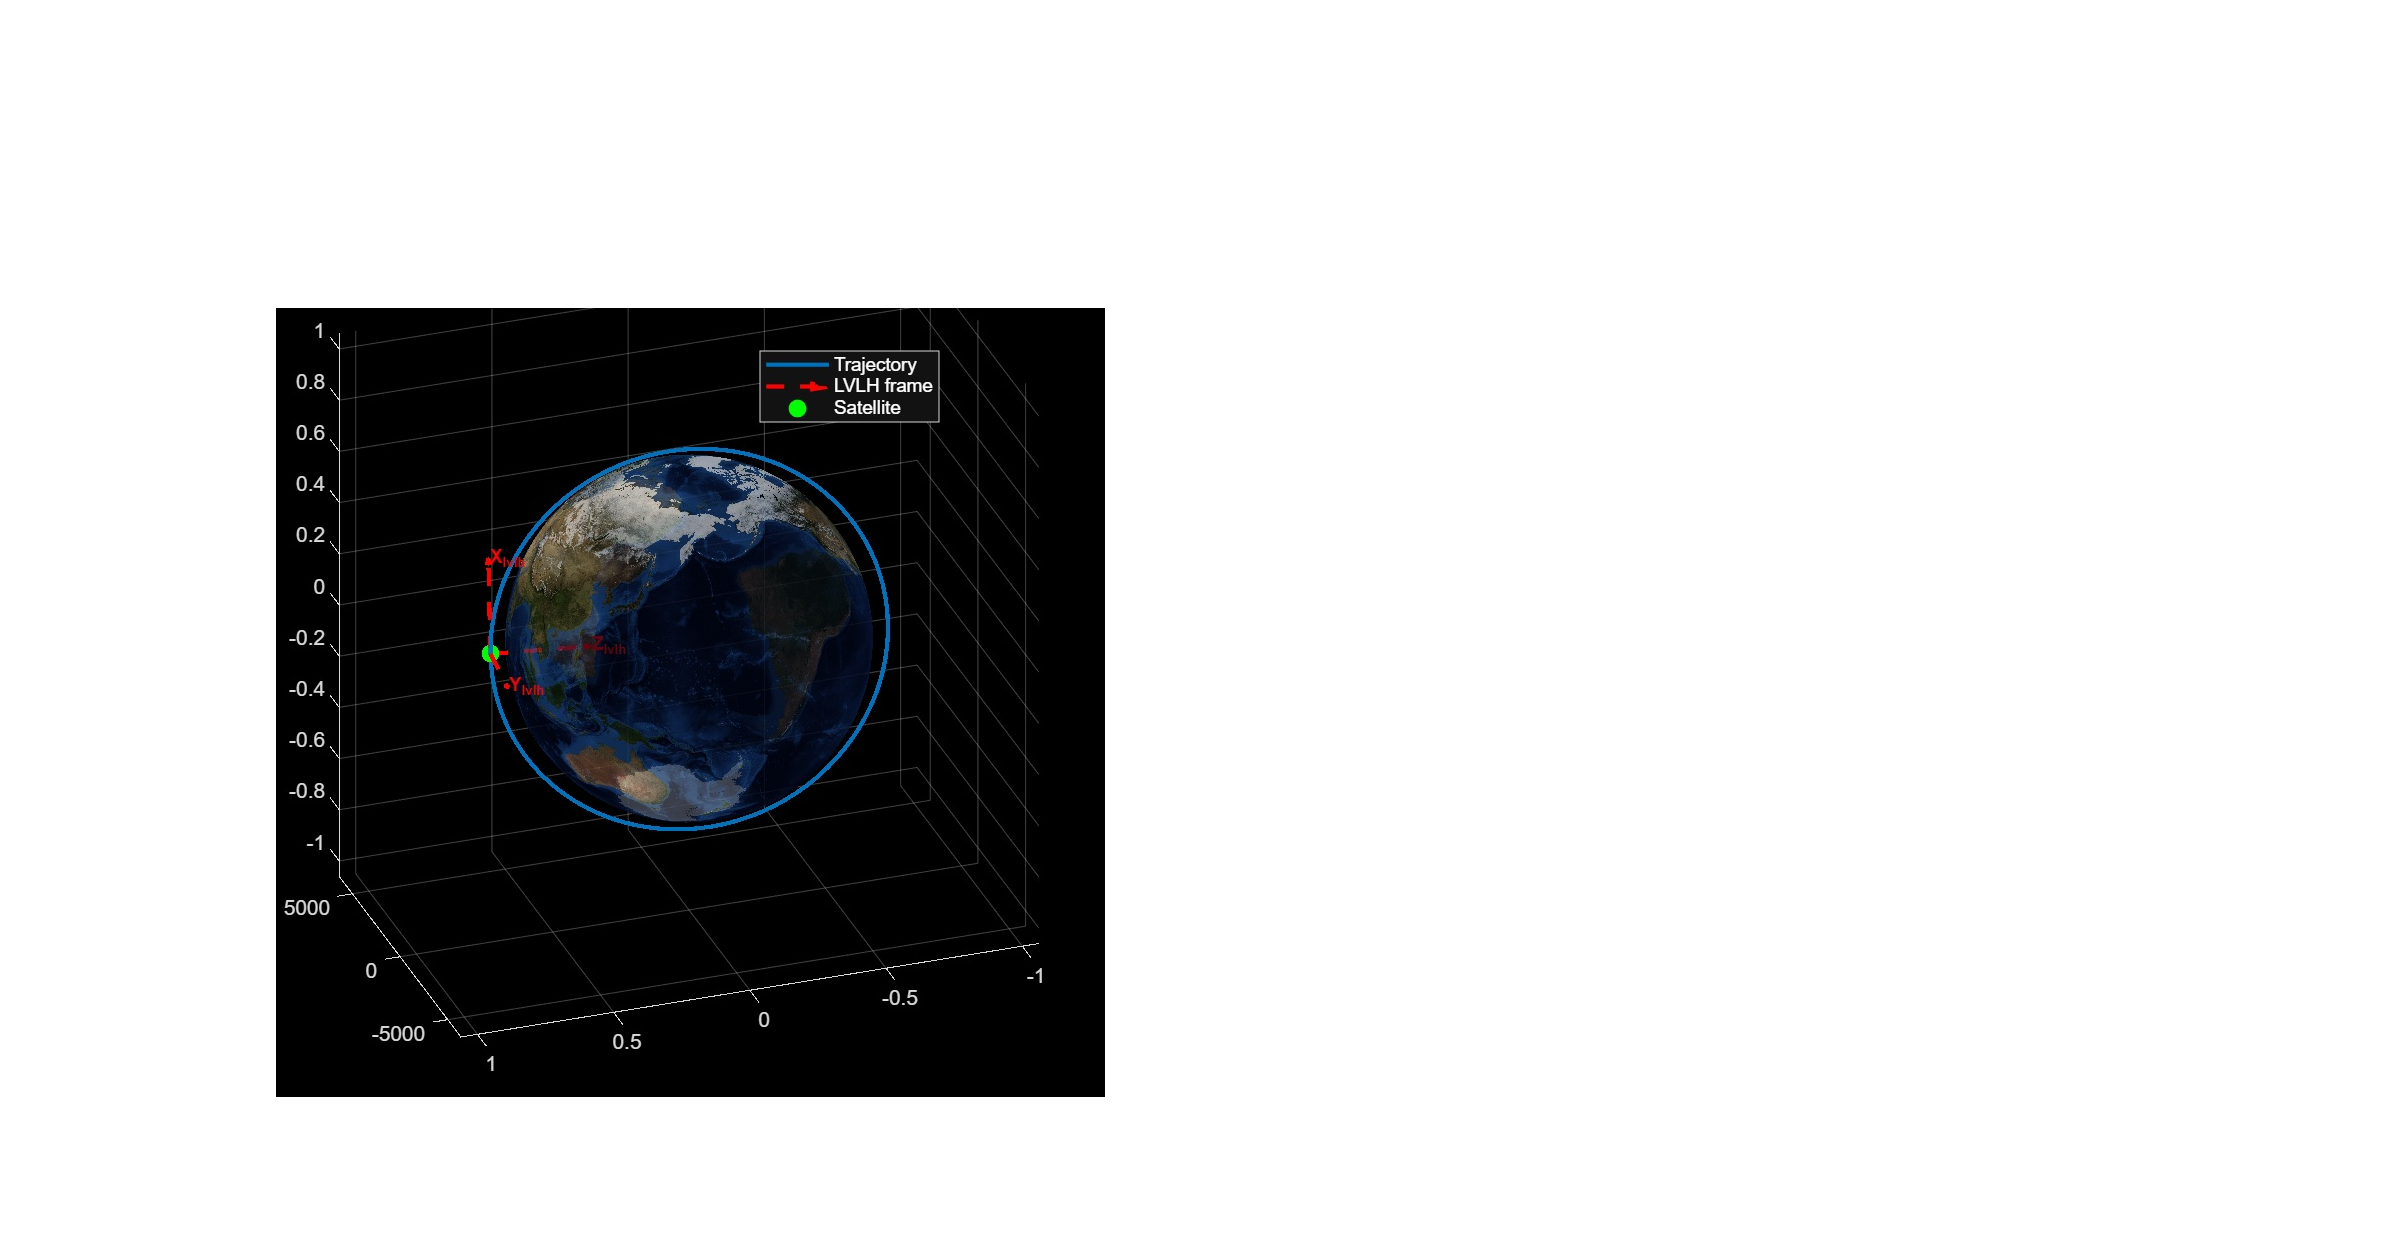
\includegraphics[height=9cm,keepaspectratio
        ]{UCSP_Pictures/satellite-propagation.pdf}
        \caption{}
        \label{fig:adcs_satellite_propagation_frames}
    \end{subfigure}
    \vspace{0.4cm}
    \begin{subfigure}[b]{\textwidth}
        \centering
        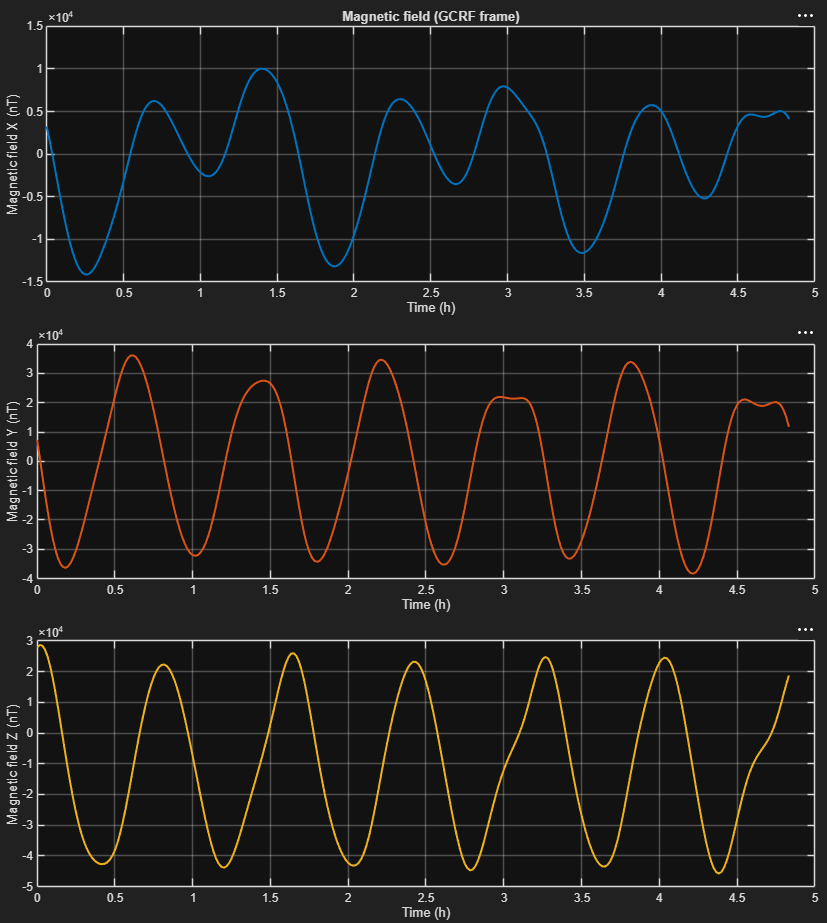
\includegraphics[height=9cm,keepaspectratio
        ]{UCSP_Pictures/magneticfield.png}
        \caption{}
        \label{fig:adcs_magnetic_field_simulation}
    \end{subfigure}
    \caption{Orbital environment simulation elements used for the ADCS analysis:
    (a) orbital propagation and reference frames;
    (b) geomagnetic field model simulation.}
    \label{fig:adcs_orbital_environment_simulation}
\end{figure}

External disturbance torques were estimated to evaluate the control authority required during the active attitude-control stages. In the rotational dynamics of Eq.~\eqref{eq:adcs_rotational_dynamics}, the disturbance torque vector \(\mathbf{T}_{d}\) is modeled as the combination of gravity-gradient torque, atmospheric-drag torque, and solar-radiation-pressure torque:

\begin{equation}
    \mathbf{T}_{d}
    =
    \mathbf{T}_{gg}
    +
    \mathbf{T}_{drag}
    +
    \mathbf{T}_{srp},
    \label{eq:adcs_total_disturbance_torque}
\end{equation}

where \(\mathbf{T}_{gg}\) is the gravity-gradient disturbance torque, \(\mathbf{T}_{drag}\) is the atmospheric-drag disturbance torque, and \(\mathbf{T}_{srp}\) is the solar-radiation-pressure disturbance torque. The environmental and surface parameters used for the SAT-ABC disturbance analysis are summarized in Table~\ref{tab:adcs_disturbance_params}.

\begin{table}[ht]
\centering
\caption{Environmental disturbance parameters and surface properties used for the SAT-ABC disturbance-torque analysis.}
\label{tab:adcs_disturbance_params}
\begin{tabular}{lcl}
\hline
\textbf{Parameter} & \textbf{Value} & \textbf{Description} \\ \hline
\(A_{x\pm}, A_{y\pm}\) & \(0.06~\mathrm{m}^2\) & Side face areas \((0.2 \times 0.3~\mathrm{m})\) \\
\(A_{z\pm}\) & \(0.04~\mathrm{m}^2\) & Top/bottom face areas \((0.2 \times 0.2~\mathrm{m})\) \\
\(q_{\mathrm{ref}}\) & 0.62 & Reflectivity coefficient for Al 6061-T6 \\
\(C_d\) & 2.2 & Aerodynamic drag coefficient \\
\(\mathbf{r}_{\mathrm{cp-cg}}\) & \([0.01, -0.005, 0.02]^T~\mathrm{m}\) & CoP-to-CoG offset vector \\ \hline
\end{tabular}
\end{table}

Figure~\ref{fig:adcs_environmental_torque_analysis} shows the resulting environmental disturbance torques for the SAT-ABC configuration, modeled as a free-rotating rigid body. The first profile summarizes the individual environmental disturbance components over the simulated interval, while the second profile shows the resulting total disturbance torque excluding the gravity-gradient contribution, as presented in the original simulation output. A summary of the maximum disturbance-torque components is provided in Table~\ref{tab:adcs_disturbances}. These values are used as reference disturbance levels for the preliminary assessment of control authority and robustness.

\begin{figure}[htbp]
    \centering
    \begin{subfigure}[b]{\textwidth}
        \centering
        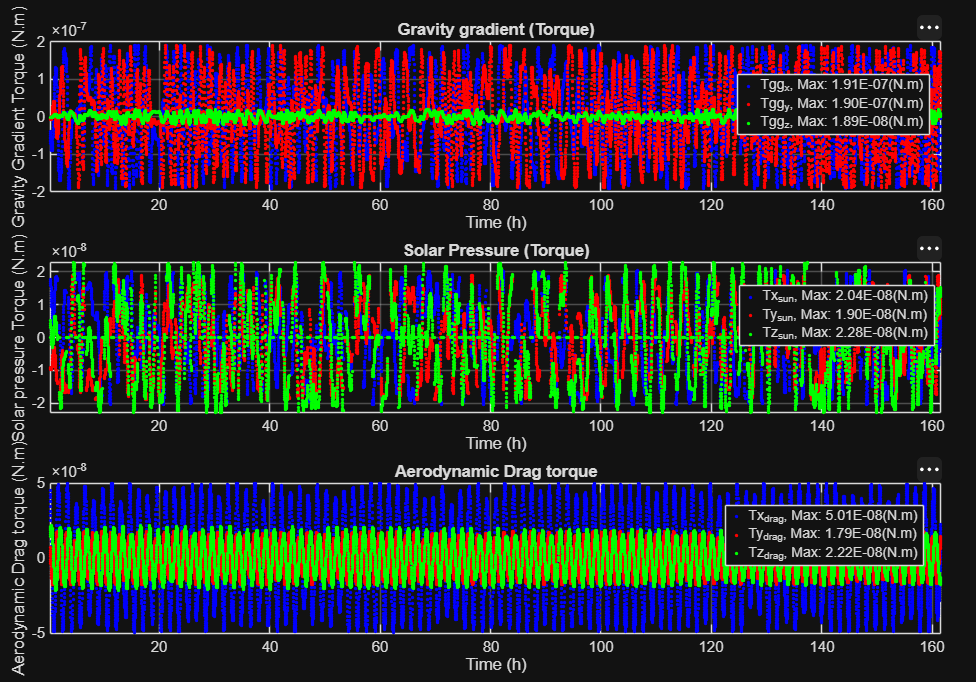
\includegraphics[height=9cm, keepaspectratio
        ]{UCSP_Pictures/Torque_disturbances_v1.png}
        \caption{}
        \label{fig:adcs_satabc_disturbances}
    \end{subfigure}
    \vspace{0.35cm}
    \begin{subfigure}[b]{\textwidth}
        \centering
        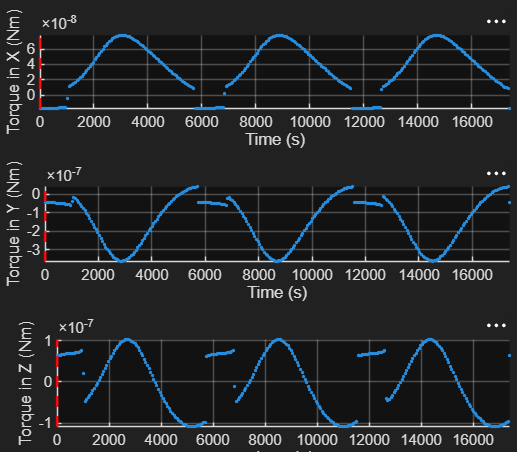
\includegraphics[height=9cm, keepaspectratio
        ]{UCSP_Pictures/Torque_disturbances.png}
        \caption{}
        \label{fig:adcs_total_torque_disturbances}
    \end{subfigure}
    \caption{Environmental disturbance torque analysis for the SAT-ABC configuration:
    (a) environmental disturbance torques acting on SAT-ABC;
    (b) total disturbance torque for SAT-ABC, excluding gravity-gradient torque.}
    \label{fig:adcs_environmental_torque_analysis}
\end{figure}

\begin{table}[ht]
\centering
\caption{Maximum disturbance torques for the SAT-ABC configuration.}
\label{tab:adcs_disturbances}
\begin{tabular}{l c c c c}
\toprule
\textbf{Torque} & \textbf{Max \(T_x\) (Nm)} & \textbf{Max \(T_y\) (Nm)} & \textbf{Max \(T_z\) (Nm)} & \textbf{Mag. (Nm)} \\
\midrule
Gravity gradient & \(1.91 \times 10^{-7}\) & \(1.90 \times 10^{-7}\) & \(1.90 \times 10^{-8}\) & \(2.70 \times 10^{-7}\) \\
Solar pressure & \(9.94 \times 10^{-9}\) & \(1.25 \times 10^{-8}\) & \(1.67 \times 10^{-8}\) & \(2.31 \times 10^{-8}\) \\
Aerodynamic torque & \(1.47 \times 10^{-8}\) & \(4.85 \times 10^{-8}\) & \(4.98 \times 10^{-8}\) & \(7.10 \times 10^{-8}\) \\
\textbf{Total} & \(\mathbf{2.16 \times 10^{-7}}\) & \(\mathbf{2.51 \times 10^{-7}}\) & \(\mathbf{8.55 \times 10^{-8}}\) & \(\mathbf{3.42 \times 10^{-7}}\) \\
\bottomrule
\end{tabular}
\end{table}

The supplementary orbital-position, velocity, and acceleration profiles used to verify the propagation environment are provided in Appendix~\ref{app:adcs_detailed_models}.

\newpage
\subsubsection{Sensor and Actuator Models}
\label{subsub:adcs_sensor_actuator_models}
The ADCS simulation framework includes representative sensor and actuator models to evaluate the attitude-determination and control functions required during the active pre-separation stages. The main assumptions and governing relations of these models are summarized in this subsection, while the complete sensor-error equations, ADC quantization model, digital filtering implementation, and actuator internal dynamics are provided in Appendix~\ref{app:adcs_detailed_models}. The sensor models provide simulated measurements of angular velocity and reference vectors, while the actuator models convert commanded control actions into physically constrained torques applied to the satellite body.

The sensor set considered in the simulation includes an Inertial Measurement Unit (IMU), magnetometer measurements, and reference-vector measurements for attitude determination. The IMU model includes gyroscope scale-factor errors, axis misalignment, bias instability modeled as a random walk process, and additive measurement noise. Magnetometer measurements are used to provide the local geomagnetic-field vector required by the magnetic attitude-control algorithms. Sun-vector and star-tracker-based reference measurements are considered for attitude-estimation convergence during the settling and pointing modes.

The gyroscope measurement model is represented in general form as

\begin{equation}
    \tilde{\boldsymbol{\omega}}_{\mathrm{raw}}(t)
    =
    \mathbf{T}_{\mathrm{ma}}
    \mathbf{T}_{\mathrm{sf}}
    \boldsymbol{\omega}(t)
    +
    \mathbf{b}_{g}(t)
    +
    \boldsymbol{\eta}_{g}(t),
    \label{eq:adcs_gyro_measurement}
\end{equation}

where \(\tilde{\boldsymbol{\omega}}_{\mathrm{raw}}(t)\) is the raw gyroscope measurement, \(\mathbf{T}_{\mathrm{sf}}\) is the scale-factor matrix, \(\mathbf{T}_{\mathrm{ma}}\) is the axis-misalignment matrix, \(\mathbf{b}_{g}(t)\) is the gyroscope bias, and \(\boldsymbol{\eta}_{g}(t)\) is the gyroscope measurement noise. The bias is propagated using a random-walk model, allowing slow sensor drift to be represented during the attitude-determination simulations.

The accelerometer, magnetometer, and reference-vector measurements are modeled by rotating the corresponding inertial-frame reference vectors into the satellite body frame and adding representative bias and noise terms. In general, these measurements can be expressed as

\begin{equation}
    \tilde{\mathbf{y}}_{\mathrm{raw}}
    =
    \mathbf{T}_{\mathrm{ma}}
    \mathbf{T}_{\mathrm{sf}}
    \left(
        \mathbf{R}(\mathbf{q})^{T}
        \mathbf{y}_{I}
    \right)
    +
    \mathbf{b}_{y}
    +
    \boldsymbol{\eta}_{y},
    \label{eq:adcs_reference_vector_measurement}
\end{equation}

where \(\mathbf{y}_{I}\) is the corresponding inertial-frame reference vector, \(\mathbf{R}(\mathbf{q})\) is the attitude rotation matrix associated with the quaternion \(\mathbf{q}\), \(\mathbf{b}_{y}\) is the measurement bias, and \(\boldsymbol{\eta}_{y}\) is the measurement noise. This general model is used to represent the accelerometer, magnetometer, and Sun-vector measurements included in the simulation.

The actuator set considered in the simulation includes magnetorquers and reaction wheels. Magnetorquers are used for detumbling and magnetic attitude-control functions. The commanded magnetic dipole is limited by the actuator saturation and by the available bus voltage. The realized magnetic dipole is then mapped to the satellite body frame using the magnetorquer configuration matrix. The resulting magnetic control torque is given by

\begin{equation}
    \boldsymbol{\tau}_{\mathrm{mtq}}
    =
    \left(
        \mathbf{W}_{\mathrm{mtq}}
        \mathbf{m}_{\mathrm{real}}
    \right)
    \times
    \mathbf{B}_{\mathrm{body}},
    \label{eq:adcs_mtq_torque}
\end{equation}

where \(\mathbf{W}_{\mathrm{mtq}}\) is the magnetorquer configuration matrix, \(\mathbf{m}_{\mathrm{real}}\) is the realized magnetic dipole vector after saturation and voltage limitations, and \(\mathbf{B}_{\mathrm{body}}\) is the local geomagnetic-field vector expressed in the body frame.

Reaction wheels are included for pointing-control analyses that require internal torque generation. The reaction-wheel assembly maps wheel momentum variation into body-frame control torque through the reaction-wheel configuration matrix. For each wheel, the generated torque is associated with the time variation of the wheel angular momentum and is computed as

\begin{equation}
    \tau_{\mathrm{rw},j}
    =
    J_{\mathrm{rw}}
    \frac{
        \omega_{\mathrm{rw},j}(t)
        -
        \omega_{\mathrm{rw},j}(t-\Delta t)
    }{\Delta t},
    \label{eq:adcs_rw_torque}
\end{equation}

where \(J_{\mathrm{rw}}\) is the rotor inertia and \(\omega_{\mathrm{rw},j}\) is the angular rate of the \(j\)-th reaction wheel.

These models provide the measurement and actuation basis for the detumbling, attitude-determination, and pointing-control simulations presented in the following subsections.

\subsection{ADCS Analysis for the SAT-ABC Configuration}
\label{sub:adcs_satabc_analysis}

The SAT-ABC configuration corresponds to the integrated spacecraft formed by SAT-A, SAT-B, and SAT-C before the release of the coupled SAT-BC system. During Mission Stage~1, the ADCS must reduce the initial angular rate of the integrated spacecraft, support attitude-determination convergence, and orient the spacecraft for the release of SAT-BC. The following analysis focuses on the active ADCS functions required during Steps~1.2--1.4 of the mission concept of operations.

\subsubsection{Initial Acquisition and Detumbling}
\label{subsub:adcs_satabc_detumbling}

After release from the deployer, SAT-ABC may present a non-zero initial angular rate. The initial acquisition sequence is represented at the functional level by a set of initialization and coarse-attitude-determination activities before the detumbling controller is activated. These activities include verification of the ADCS sensor and actuator status, initial gyroscope and magnetometer bias characterization, synchronization of the satellite body axes with the flight software reference frames, and coarse attitude determination using Sun and geomagnetic reference vectors.

The detumbling maneuver is performed using an orthogonal magnetorquer configuration based on the iADCS400 module. The objective is to reduce the initial angular rate, considered up to \(\pm 5~\mathrm{deg/s}\), to a stable condition below \(1~\mathrm{deg/s}\). A pure B-dot controller is used for this purpose. The analytical magnetic-field derivative is estimated from the measured angular velocity and magnetic-field vector as

\begin{equation}
    \dot{\mathbf{B}}_{\mathrm{analytical}}
    =
    -
    \boldsymbol{\omega}_{\mathrm{meas}}
    \times
    \mathbf{B}_{\mathrm{meas}},
    \label{eq:adcs_satabc_bdot_analytical}
\end{equation}

where \(\boldsymbol{\omega}_{\mathrm{meas}}\) is the measured angular velocity and \(\mathbf{B}_{\mathrm{meas}}\) is the measured geomagnetic-field vector expressed in the body frame. The commanded magnetic dipole is defined as

\begin{equation}
    \mathbf{m}_{\mathrm{cmd}}
    =
    -
    K_{\mathrm{bdot}}
    f_{\mathrm{bang\mbox{-}bang}}
    \dot{\mathbf{B}}_{\mathrm{analytical}},
    \label{eq:adcs_satabc_bdot_dipole_command}
\end{equation}

where \(K_{\mathrm{bdot}}\) is the theoretical B-dot gain and \(f_{\mathrm{bang\mbox{-}bang}}\) is a scaling factor used to drive the coils close to their saturation region and increase rotational-energy dissipation. The theoretical base gain is computed as

\begin{equation}
    K_{\mathrm{bdot}}
    =
    \frac{
        4\pi
        \left(
            1 + \sin i
        \right)
        I_{\min}
    }{
        T_{\mathrm{orb}}
        B_{\mathrm{avg}}^{2}
    },
    \label{eq:adcs_satabc_bdot_gain}
\end{equation}

where \(i\) is the orbital inclination, \(I_{\min}\) is the minimum principal moment of inertia, \(T_{\mathrm{orb}}\) is the orbital period, and \(B_{\mathrm{avg}}\) is the average geomagnetic-field magnitude along the orbit.

The B-dot gain is scaled using \(f_{\mathrm{bang\mbox{-}bang}} = 10^{3}\). The stabilization threshold is set to \(\omega_{\mathrm{th}} < 1~\mathrm{deg/s}\). To avoid premature transitions caused by magnetometer noise or instantaneous angular-rate peaks, the transition logic includes a hysteresis condition with a reset threshold of \(1.2~\mathrm{deg/s}\). A hold time of \(3600~\mathrm{s}\) is then applied to verify that the detumbled state is maintained before transitioning to the next ADCS operating mode.

The nominal parameters used for the SAT-ABC detumbling simulations are summarized in Table~\ref{tab:adcs_satabc_detumbling_params}. These parameters include the magnetorquer limits and the representative IMU noise characteristics used in the Monte Carlo analysis to verify the robustness of the SAT-ABC detumbling strategy under the modeled sensor and actuator limitations. Figure~\ref{fig:adcs_satabc_detumbling_montecarlo} shows the angular-velocity convergence and the statistical distribution of the detumbling times. 

\begin{table}[htbp]
\centering
\caption{Nominal parameters used for the SAT-ABC detumbling simulations.}
\label{tab:adcs_satabc_detumbling_params}
\begin{tabular}{lll}
\toprule
\textbf{Parameter / Component} & \textbf{Symbol / Variable} & \textbf{Value / Unit} \\
\midrule
\multicolumn{3}{l}{\textbf{Actuators: Magnetorquers based on iADCS400}} \\
Maximum power & \(P_{\max}\) & \(600~\mathrm{mW}\) \\
Operating voltage & \(V_{\mathrm{op}}\) & \(5~\mathrm{V}\) \\
Nominal magnetic dipole & \(m_{\mathrm{nom}}\) & \(0.4~\mathrm{A\,m^{2}}\) \\
Residual dipole & \(\mathbf{m}_{\mathrm{rem}}\) & \([0.004, -0.002, 0.003]^T~\mathrm{A\,m^{2}}\) \\
Linearity factor & \(k_{\mathrm{lin}}\) & \(2.0\) \\
\midrule
\multicolumn{3}{l}{\textbf{Sensors: IMU magnetometer and gyroscope based on iADCS400}} \\
Magnetometer standard deviation & \(\sigma_{\mathrm{mag}}\) & \(150~\mathrm{nT}\) \\
Magnetometer resolution & \(\mathrm{res}_{\mathrm{mag}}\) & \(10~\mathrm{nT}\) \\
Gyroscope noise & \(\eta_{\mathrm{gyro}}\) & \(0.05~\mathrm{deg/s}\) \\
Bias random walk & \(\sigma_{\mathrm{RW}}\) & \(0.005~\mathrm{deg/s}/\sqrt{\mathrm{s}}\) \\
Gyroscope saturation range & \(\omega_{\max}\) & \(\pm 250~\mathrm{deg/s}\) \\
\bottomrule
\end{tabular}
\end{table}

\begin{figure}[htbp]
    \centering
    \includegraphics[width=1\linewidth]{UCSP_Pictures/State 1 Verification.pdf}
    \caption{Monte Carlo simulation results for the SAT-ABC detumbling mode, showing angular-velocity convergence and settling-time distributions.}
    \label{fig:adcs_satabc_detumbling_montecarlo}
\end{figure}

The results indicate that all simulated cases reached the stabilization threshold, with \(500\) out of \(500\) runs achieving \(\|\boldsymbol{\omega}\| < 1~\mathrm{deg/s}\). The first crossing of the detumbling threshold occurred with a mean time of \(0.55~\mathrm{h}\). After applying the \(3600~\mathrm{s}\) hold-time condition, the verified detumbling time had a mean value of \(1.55~\mathrm{h}\), with a maximum value of \(1.92~\mathrm{h}\). The reset threshold of \(1.2~\mathrm{deg/s}\) prevents premature transitions due to sensor noise, instantaneous angular-rate peaks, or residual dipole effects. 

Considering an orbital period of about \(96~\mathrm{min}\), the verified detumbling time remains below approximately \(1.3\) orbits. These results provide a preliminary feasibility indication for transitioning from SAT-ABC detumbling to the subsequent attitude-determination and pointing-control modes.

\subsubsection{Attitude Determination Convergence}
\label{subsub:adcs_satabc_attitude_determination}

After the SAT-ABC configuration reaches the verified detumbled state, the ADCS enters a settling interval to allow the attitude-determination algorithms to converge before initiating the velocity-vector pointing maneuver. This operating mode corresponds mainly to Step~1.3 of the mission concept of operations. During this interval, the attitude estimator uses IMU measurements together with reference-vector measurements, including a star-tracker model represented by a set of five reference vectors based on the iADCS400 characteristics.

Several Attitude and Heading Reference System (AHRS) algorithms were considered to evaluate candidate approaches for attitude estimation during this settling interval. The algorithms include deterministic vector-based methods, complementary-filter approaches, and Kalman-filter-based estimators:

\begin{itemize}
    \item \textbf{QUEST algorithm:} QUEST is a deterministic solution to Wahba's problem. It estimates the attitude quaternion by constructing Davenport's \(K\)-matrix from weighted body-frame vector observations and their corresponding inertial-frame references. The optimal quaternion is obtained from the eigenvector associated with the largest eigenvalue, providing a measurement-only attitude estimate independent of gyroscope propagation~\cite{crassidis2021spacecraft, bar1996request}.

    \item \textbf{RE-QUEST algorithm:} RE-QUEST extends QUEST by recursively updating the attitude estimate using gyroscope propagation and vector observations. It propagates an accumulated attitude-information matrix using angular-rate measurements and updates it with new reference-vector observations, allowing high-rate gyroscope data to be fused with lower-rate vector measurements~\cite{bar1996request}.

    \item \textbf{Mahony filter:} The Mahony filter is a nonlinear complementary filter that fuses gyroscope data with vector observations through proportional-integral feedback. The proportional term corrects the instantaneous attitude error, while the integral term supports gyroscope-bias compensation. Its quaternion-based implementation is suitable for embedded attitude-estimation applications~\cite{10850038}.

    \item \textbf{Madgwick filter:} The Madgwick filter estimates the attitude quaternion and gyroscope bias by combining gyroscope-based propagation with a gradient-descent correction based on vector observations. The prediction step integrates the measured angular rate, while the correction step minimizes the mismatch between measured and predicted reference vectors. The estimated quaternion rate can be expressed as

    \begin{equation}
        \dot{\mathbf{q}}_{\mathrm{est},t}
        =
        \dot{\mathbf{q}}_{\omega,t}
        -
        \beta
        \dot{\mathbf{q}}_{\epsilon,t},
        \label{eq:adcs_madgwick_estimated_rate}
    \end{equation}

    where \(\dot{\mathbf{q}}_{\omega,t}\) is the quaternion rate obtained from gyroscope propagation, \(\dot{\mathbf{q}}_{\epsilon,t}\) is the normalized correction direction obtained from the gradient of the objective function, and \(\beta\) is the filter gain~\cite{madgwick2010filter}.

    \item \textbf{Extended Kalman Filter (EKF):} The EKF is considered as a full-state nonlinear estimator with state vector
    \(\mathbf{x} = [\mathbf{q}^{T}, \mathbf{b}_{g}^{T}]^{T}\), where \(\mathbf{q}\) is the attitude quaternion and \(\mathbf{b}_{g}\) is the gyroscope bias. The covariance matrix \(\mathbf{P} \in \mathbb{R}^{7\times7}\) represents the uncertainty of the state estimate. The measurement model uses reference vectors transformed into the body frame, consistent with Eq.~\eqref{eq:adcs_reference_vector_measurement}. The predict step propagates the attitude using gyroscope measurements, while the update step corrects the state using available vector measurements.

    \item \textbf{Unscented Kalman Filter (UKF):} The UKF is considered as an alternative nonlinear estimator that propagates a set of sigma points through the quaternion kinematic model of Eq.~\eqref{eq:adcs_quaternion_kinematics}. The attitude uncertainty is represented through a three-dimensional rotation-error covariance matrix. During the correction step, the propagated sigma points are transformed into the measurement space to compare predicted and measured reference vectors, after which the Kalman gain is used to update the attitude estimate.
\end{itemize}

The preceding descriptions summarize the candidate AHRS algorithms considered for the SAT-ABC attitude-determination convergence assessment. Additional mathematical and implementation details for the deterministic vector-based methods, complementary filters, and Kalman-filter-based estimators are provided in Appendix~\ref{app:adcs_detailed_models}.

Figure~\ref{fig:adcs_satabc_ekf_process} summarizes the predict--update structure used by the EKF implementation. This structure separates high-frequency attitude propagation from lower-frequency measurement correction, allowing new sensor observations to be incorporated when available.

\begin{figure}[ht]
    \centering
    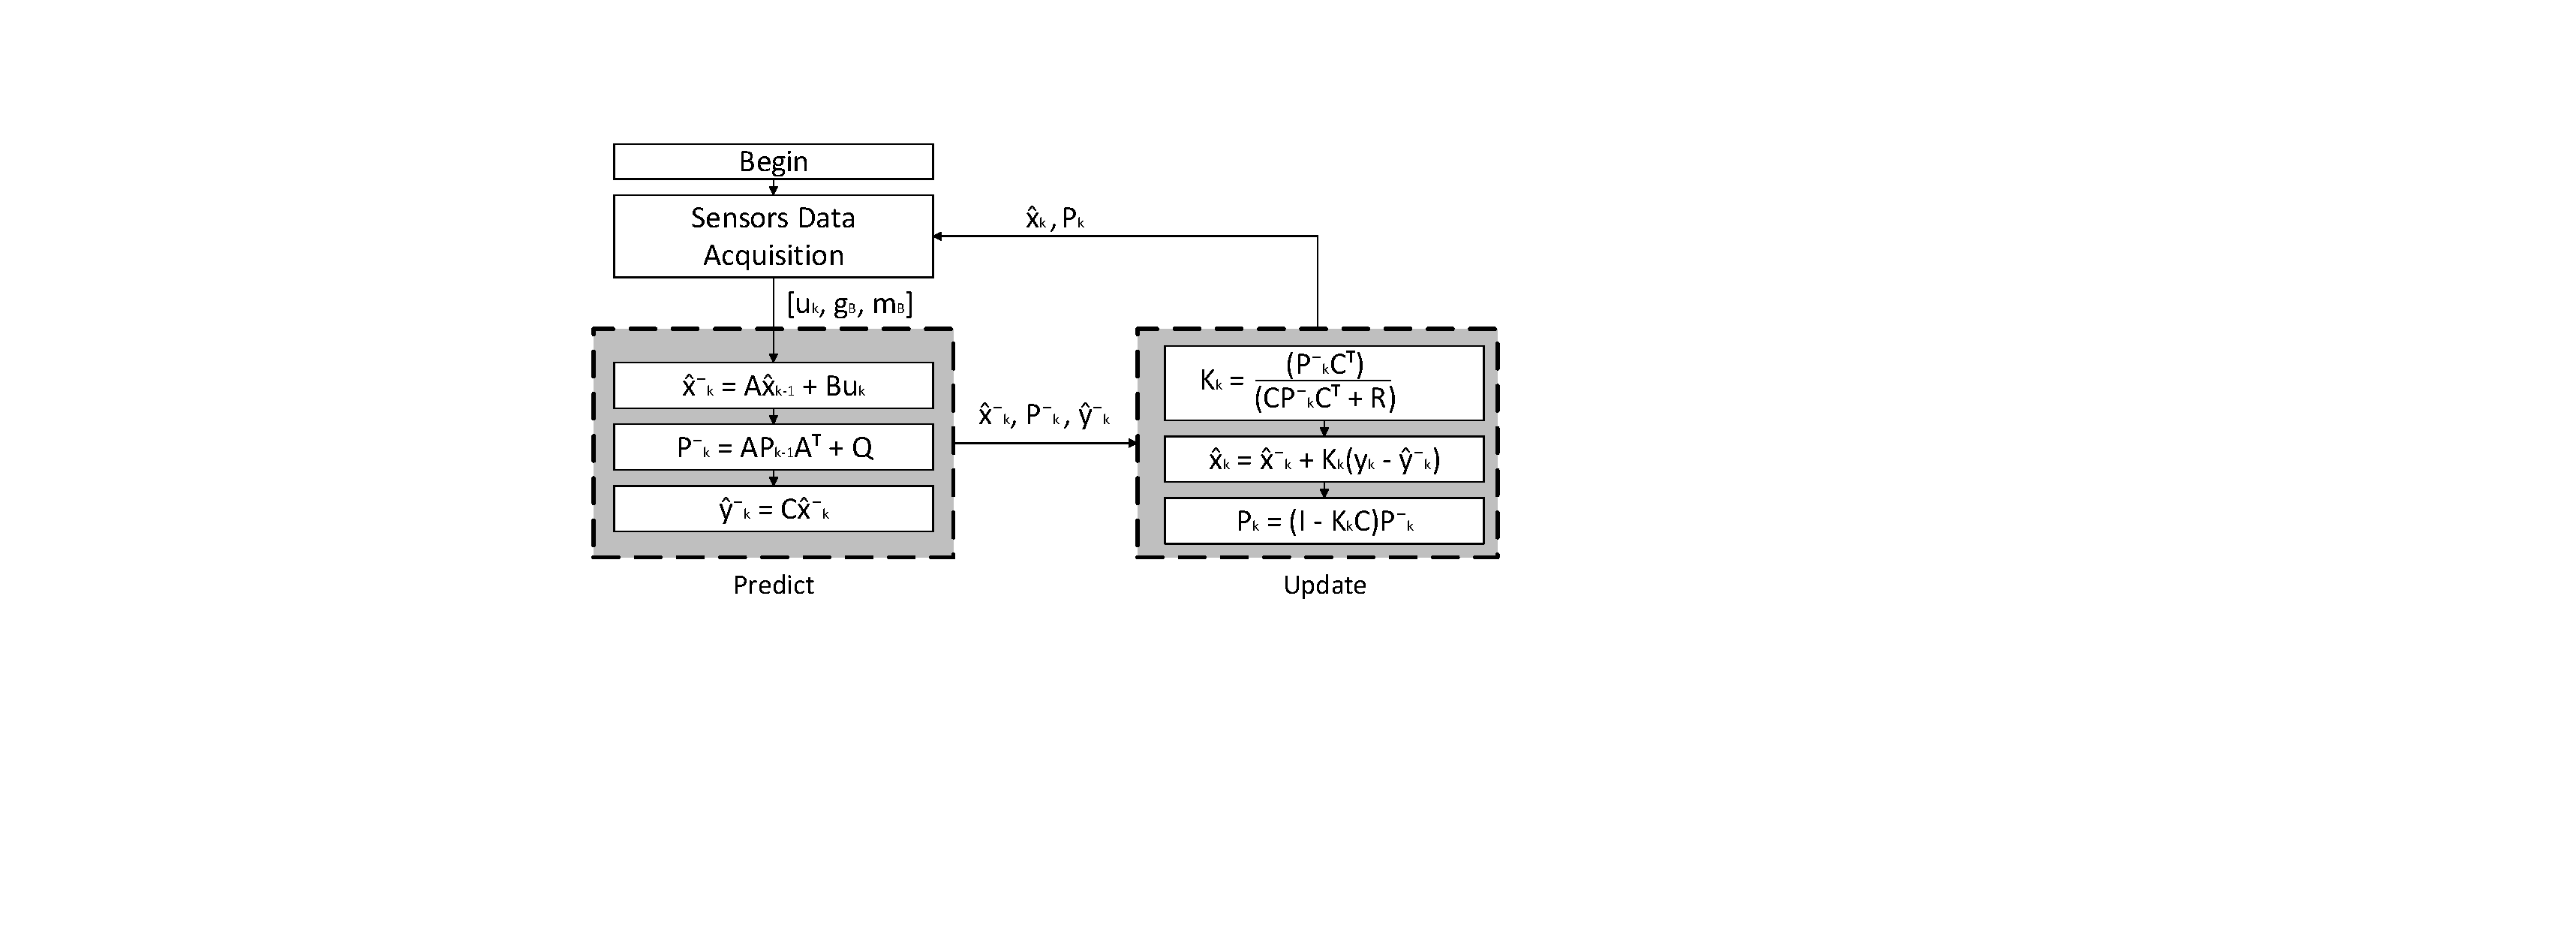
\includegraphics[width=0.55\linewidth]{UCSP_Pictures/imagen22.pdf}
    \caption{EKF predict--update process used for attitude-determination convergence assessment.}
    \label{fig:adcs_satabc_ekf_process}
\end{figure}

The settling-mode analysis supports the preliminary selection and tuning of the attitude-estimation approach before the SAT-ABC pointing maneuver. At this stage, the objective is not to define a final flight estimator, but to verify that the modeled sensor set and candidate AHRS algorithms can support attitude-determination convergence before transitioning to the velocity-vector pointing mode.

\subsubsection{Velocity-Vector Pointing Control}
\label{subsub:adcs_satabc_pointing}

After the SAT-ABC configuration reaches a verified detumbled state and the attitude-determination algorithms have converged, the ADCS must orient the spacecraft for the release of SAT-BC. This operating mode corresponds mainly to Step~1.4 of the mission concept of operations. In this preliminary analysis, the pointing objective is to align the SAT-ABC body-frame \(Z_B\)-axis with the translational velocity vector, also referred to as the ram direction.

Two nonlinear quaternion-based attitude-control approaches were evaluated for this maneuver: a conventional Quaternion Feedback Controller and the robust adaptive controller proposed by Boskovic et al.~\cite{Boskovic2004}. The attitude error is represented using the quaternion error, while the angular-rate tracking error is denoted by \(\delta\boldsymbol{\omega} = \boldsymbol{\omega} - \boldsymbol{\omega}_{d}\), where \(\boldsymbol{\omega}_{d}\) is the desired angular velocity. The control torques are assumed to be generated by the reaction-wheel assembly, consistent with the actuator model introduced in Eq.~\eqref{eq:adcs_rw_torque}.

For the Quaternion Feedback Controller, the vector-part tracking error is defined as

\begin{equation}
    \delta\boldsymbol{\beta}
    =
    \mathbf{q}_{13}
    -
    \mathbf{q}_{d,13},
    \label{eq:adcs_satabc_quaternion_vector_error}
\end{equation}

where \(\mathbf{q}_{13}\) is the vector part of the current attitude quaternion and \(\mathbf{q}_{d,13}\) is the vector part of the desired attitude quaternion. The control law is expressed as

\begin{equation}
\begin{aligned}
    \mathbf{u}
    &=
    \mathbf{P}\delta\boldsymbol{\omega}
    +
    \mathbf{K}\delta\boldsymbol{\beta}
    -
    [\boldsymbol{\omega}\times]
    \left(
        \mathbf{J}_{B}\boldsymbol{\omega}
        -
        \mathbf{J}_{rw}
        \left(
            \boldsymbol{\omega}
            +
            \boldsymbol{\Omega}
        \right)
    \right) \\
    &\quad
    -
    \mathbf{J}_{B}
    \left(
        \dot{\boldsymbol{\omega}}_{d}
        -
        [\boldsymbol{\omega}\times]\boldsymbol{\omega}_{d}
    \right),
\end{aligned}
\label{eq:adcs_satabc_quaternion_feedback_control}
\end{equation}

where \(\mathbf{u}\) is the commanded control torque, \(\mathbf{P}\) and \(\mathbf{K}\) are positive-definite gain matrices, and \(\mathbf{J}_{B}\) is the inertia tensor of the SAT-ABC body expressed in the body-fixed frame, using the representative inertia properties summarized in Table~\ref{tab:adcs_inertia_properties}. The matrix \(\mathbf{J}_{rw}\) represents the reaction-wheel inertia values along their spin axes, and \(\boldsymbol{\Omega}\) contains the reaction-wheel angular rates. The terms \(\boldsymbol{\omega}_{d}\) and \(\dot{\boldsymbol{\omega}}_{d}\) denote the desired angular velocity and angular acceleration, respectively.

Using the Quaternion Feedback Controller of Eq.~\eqref{eq:adcs_satabc_quaternion_feedback_control}, the velocity-vector pointing simulation was performed by skipping the detumbling state and assuming unitary controller gains. Figure~\ref{fig:adcs_satabc_quaternion_feedback_results} shows the resulting attitude quaternions, equivalent Euler-angle error, and required control torque. The quaternion error remains around \(0.3^\circ\), indicating good pointing performance under the assumed conditions. However, this controller requires accurate knowledge of the satellite inertia tensor.

\begin{figure}[htbp]
    \centering
    \begin{subfigure}[b]{\textwidth}
        \centering
        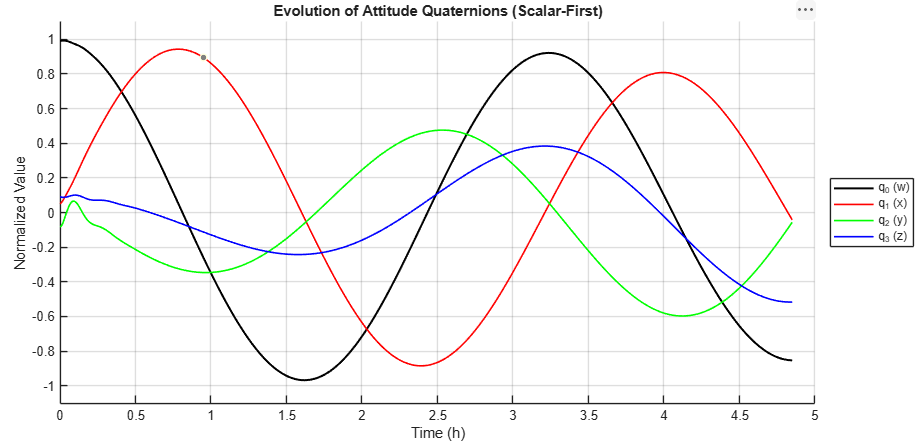
\includegraphics[width=0.82\linewidth]{UCSP_Pictures/SAT-ABC_Attitude_quaternions.png}
        \caption{SAT-ABC attitude quaternions.}
        \label{fig:adcs_satabc_quaternion_feedback_attitude}
    \end{subfigure}
    \vspace{0.3cm}
    \begin{subfigure}[b]{\textwidth}
        \centering
        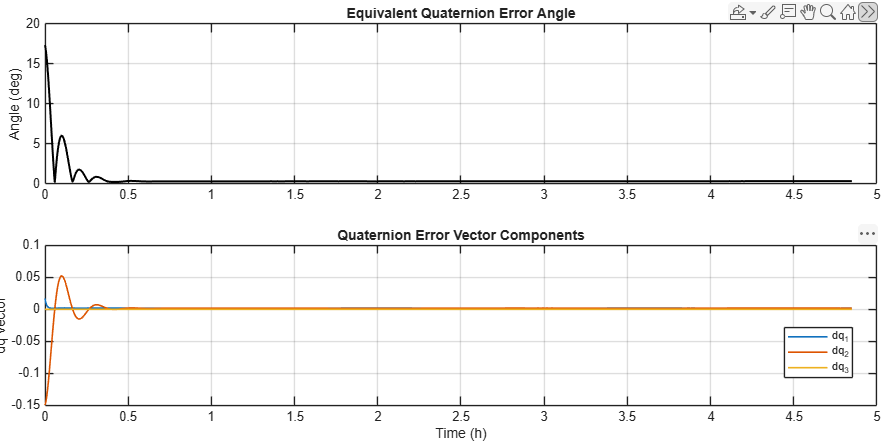
\includegraphics[width=0.82\linewidth]{UCSP_Pictures/SAT-ABC_Attitude_quaternions_error.png}
        \caption{Quaternion error and equivalent Euler-angle error.}
        \label{fig:adcs_satabc_quaternion_feedback_error}
    \end{subfigure}
    \vspace{0.3cm}
    \begin{subfigure}[b]{\textwidth}
        \centering
        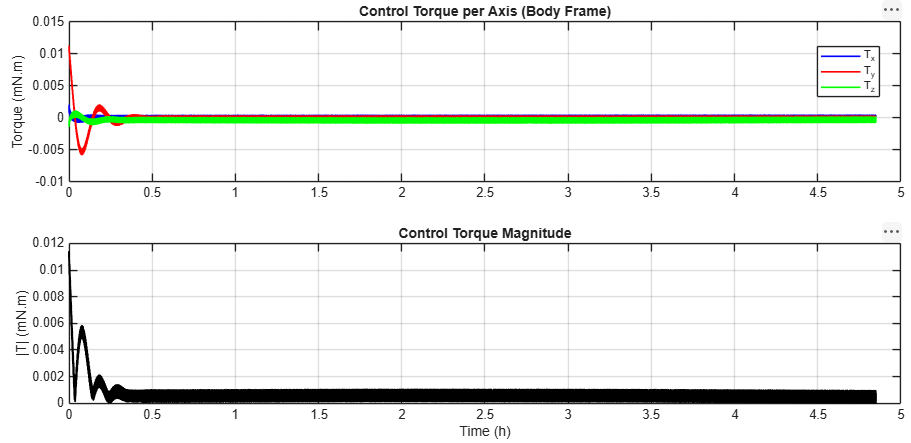
\includegraphics[width=0.82\linewidth]{UCSP_Pictures/SAT-ABC_triaxial_Torque.png}
        \caption{Required triaxial control torque.}
        \label{fig:adcs_satabc_quaternion_feedback_torque}
    \end{subfigure}
    \caption{SAT-ABC velocity-vector pointing results using the Quaternion Feedback Controller:
    (a) attitude quaternions;
    (b) quaternion error and equivalent Euler-angle error;
    (c) required control torque.}
    \label{fig:adcs_satabc_quaternion_feedback_results}
\end{figure}

Because the satellite inertia tensor is difficult to measure precisely before flight, the robust adaptive controller proposed by Boskovic et al.~\cite{Boskovic2004} was also evaluated. This controller is based on a variable-structure approach and is intended to reduce attitude and angular-velocity errors without requiring prior exact knowledge of the inertia tensor. The control law is defined as

\begin{equation}
    -u_i(t)
    =
    -u_{\max}
    \frac{
        s_i(t)
    }{
        |s_i(t)| + k^2(t)\delta_k
    },
    \qquad
    i = 1,2,3,
    \label{eq:adcs_satabc_boskovic_control}
\end{equation}

where \(\delta_k\) is a positive constant, \(k(t)\) is the adaptive gain, and \(u_{\max}\) is the torque limit applied to each control axis. The corresponding sliding vector is defined as

\begin{equation}
    \mathbf{s}(t)
    =
    \delta\boldsymbol{\omega}(t)
    +
    k^2(t)\delta\mathbf{q}_{13}(t).
    \label{eq:adcs_satabc_boskovic_sliding_vector}
\end{equation}

In Eq.~\eqref{eq:adcs_satabc_boskovic_sliding_vector}, \(\delta\mathbf{q}_{13}\) denotes the vector part of the quaternion attitude error, and \(\delta\boldsymbol{\omega}\) denotes the angular-rate tracking error. 

The full adaptive-gain adjustment law used in the Boskovic controller is provided in Appendix~\ref{app:adcs_detailed_models}. In the main analysis, the controller is assessed through the resulting attitude response, pointing error, and required control torque.

Figure~\ref{fig:adcs_satabc_boskovic_results} shows the SAT-ABC velocity-vector pointing results obtained with the Boskovic controller. The results include the attitude quaternions aligned with the velocity-vector reference, the quaternion error with its equivalent Euler-angle representation, and the required control torque. In this preliminary comparison, the Boskovic controller improves the convergence behavior relative to the conventional quaternion feedback controller when the inertia tensor is not assumed to be precisely known. This result is obtained under the assumption of ideal actuators and is therefore interpreted as a preliminary indication of robust-control feasibility rather than a final actuator-level verification.

\begin{figure}[htbp]
    \centering
    \begin{subfigure}[b]{\textwidth}
        \centering
        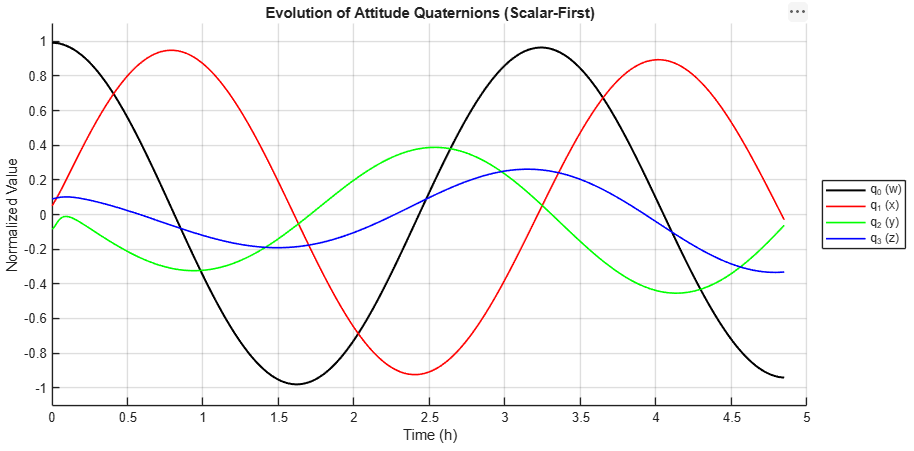
\includegraphics[width=0.82\linewidth]{UCSP_Pictures/SAT-ABC_Attitude_quaternions_bosk.png}
        \caption{SAT-ABC attitude quaternions.}
        \label{fig:adcs_satabc_boskovic_attitude}
    \end{subfigure}
    \vspace{0.3cm}
    \begin{subfigure}[b]{\textwidth}
        \centering
        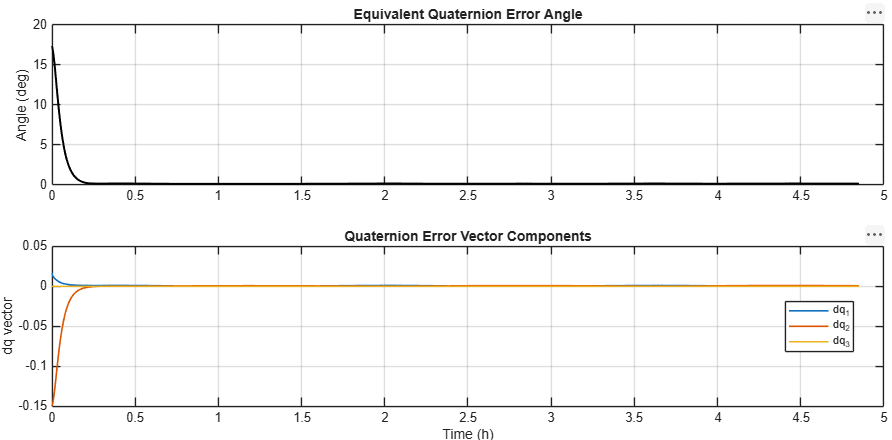
\includegraphics[width=0.82\linewidth]{UCSP_Pictures/SAT-ABC_Attitude_quaternions_error_bosk.png}
        \caption{Quaternion error and equivalent Euler-angle error.}
        \label{fig:adcs_satabc_boskovic_error}
    \end{subfigure}
    \vspace{0.3cm}
    \begin{subfigure}[b]{\textwidth}
        \centering
        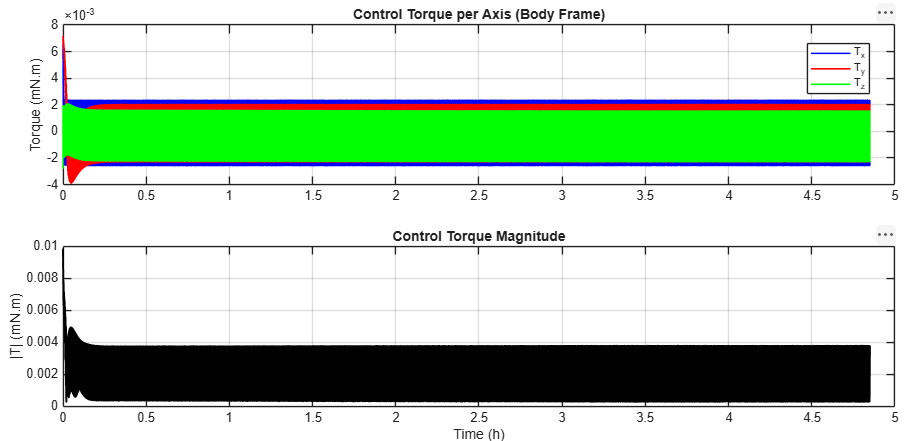
\includegraphics[width=0.82\linewidth]{UCSP_Pictures/SAT-ABC_triaxial_Torque_bosk.png}
        \caption{Required triaxial control torque.}
        \label{fig:adcs_satabc_boskovic_torque}
    \end{subfigure}
    \caption{SAT-ABC velocity-vector pointing results using the Boskovic robust controller:
    (a) attitude quaternions;
    (b) quaternion error and equivalent Euler-angle error;
    (c) required control torque.}
    \label{fig:adcs_satabc_boskovic_results}
\end{figure}

The SAT-ABC pointing-control analysis indicates that velocity-vector alignment is feasible in simulation using nonlinear quaternion-based control. The conventional quaternion feedback controller provides low pointing error when the inertia tensor is known, while the Boskovic robust controller offers a candidate approach for reducing sensitivity to inertia uncertainty. Further work is required to evaluate the selected controller with non-ideal actuator dynamics, reaction-wheel saturation limits, disturbance torques, and the final inertia properties of the integrated SAT-ABC configuration.

\subsection{ADCS Analysis for the SAT-BC Configuration}
\label{sub:adcs_satbc_analysis}

The SAT-BC configuration corresponds to the coupled SAT-B/SAT-C body after its release from SAT-A and before the internal SAT-B/SAT-C separation command. During Mission Stage~2, the ADCS must reduce the angular rate of the coupled body, verify that a stable attitude condition has been reached, and support the nadir-pointing orientation required before tether deployment. The following analysis focuses on the active ADCS functions required during Steps~2.2--2.4 of the mission concept of operations.

\subsubsection{Initial Acquisition and Detumbling}
\label{subsub:adcs_satbc_detumbling}

After release from SAT-A, the SAT-BC configuration may present a non-zero initial angular rate. As in the SAT-ABC case, the initial acquisition sequence is represented at the functional level by verification and coarse-attitude-determination activities before activating the detumbling controller. These activities include verification of the ADCS sensor and actuator status, gyroscope and magnetometer bias characterization during the initial free-drift condition, synchronization of the SAT-BC geometric axes with the flight-software reference frames, and coarse attitude determination using Sun and geomagnetic reference vectors.

The SAT-BC detumbling maneuver is analyzed using a magnetorquer-only configuration. The representative inertia properties are taken from the SAT-BC case summarized in Table~\ref{tab:adcs_inertia_properties}, while the sensor and actuator parameters used in the simulation are summarized in Table~\ref{tab:adcs_satbc_detumbling_params}. This configuration reflects the intended use of magnetic actuation for initial angular-rate reduction before the nadir-pointing preparation step.

The same B-dot control formulation introduced for the SAT-ABC detumbling analysis in Eqs.~\eqref{eq:adcs_satabc_bdot_analytical}--\eqref{eq:adcs_satabc_bdot_gain} is applied to the SAT-BC configuration, using the SAT-BC inertia properties summarized in Table~\ref{tab:adcs_inertia_properties} and the sensor and actuator parameters listed in Table~\ref{tab:adcs_satbc_detumbling_params}.

\begin{table}[htbp]
\centering
\caption{Nominal parameters used for the SAT-BC detumbling simulations.}
\label{tab:adcs_satbc_detumbling_params}
\begin{tabular}{lll}
\toprule
\textbf{Parameter / Component} & \textbf{Value} & \textbf{Unit} \\
\midrule
\multicolumn{3}{l}{\textbf{Actuators: Magnetorquers}} \\
Nominal / maximum power, \(P\) & 0.360 & W \\
Operating voltage, \(V\) & 5.0 & V \\
Dimensions, \(w \times h \times l\) & \(30 \times 30 \times 30\) & mm \\
Nominal / maximum dipole & 0.1 & \(\mathrm{A\,m^2}\) \\
Residual dipole, \(\mathbf{m}_{\mathrm{res}}\) & \([0.004, -0.002, 0.003]^T\) & \(\mathrm{A\,m^2}\) \\
Linearity factor & 2.0 & -- \\
\midrule
\multicolumn{3}{l}{\textbf{Sensors: Magnetometer}} \\
Noise standard deviation, \(\sigma_{\mathrm{mag}}\) & \(150.00 \times 10^{-9}\) & T \\
Resolution & \(10.00 \times 10^{-9}\) & T \\
Standard deviation norm & 0.5 & -- \\
Filter time constant, \(\tau\) & 0.5 & s \\
\midrule
\multicolumn{3}{l}{\textbf{Sensors: Gyroscope (IMU)}} \\
Scale factor & \([0.005, 0.005, 0.005]^T\) & -- \\
Misalignment matrix, \(\mathbf{M}_{\mathrm{mis}}\) &
\(\begin{bmatrix}
0 & 0.001 & 0.001 \\
0.001 & 0 & 0.001 \\
0.001 & 0.001 & 0
\end{bmatrix}\) & rad \\
White noise, \(\eta_g\) & 0.05 & deg/s \\
Bias instability, \(\sigma_{\mathrm{RW}}\) & 0.005 & \(\mathrm{deg/s}/\sqrt{\mathrm{s}}\) \\
Filter time constant, \(\tau\) & 0.1 & s \\
Saturation limits, \(y_{\min}, y_{\max}\) & \(\pm 250\) & deg/s \\
ADC resolution & 16 & bits \\
Reference voltage, \(V_{\mathrm{ref}}\) & 3.3 & V \\
\bottomrule
\end{tabular}
\end{table}

A Monte Carlo analysis was performed to verify the robustness of the SAT-BC detumbling strategy under the modeled sensor and actuator limitations. Figure~\ref{fig:adcs_satbc_detumbling_montecarlo} shows the angular-velocity convergence and the statistical distribution of the detumbling times.

\begin{figure}[htbp]
    \centering
    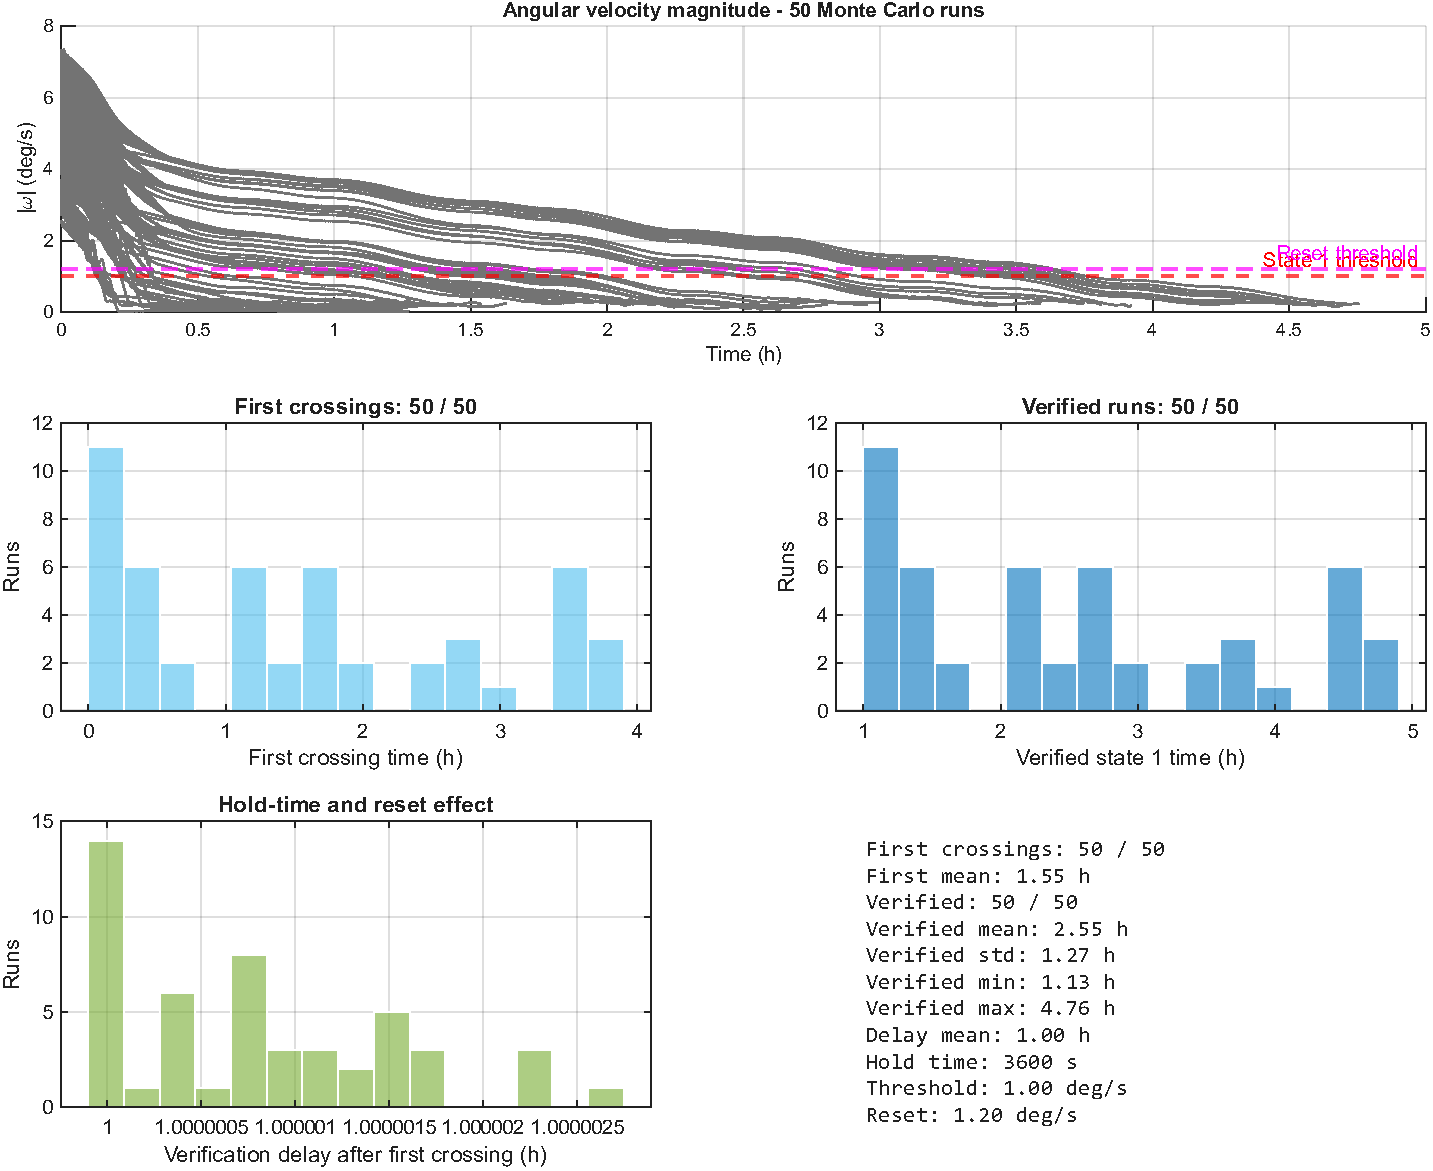
\includegraphics[width=0.9\linewidth]{UCSP_Pictures/State 1 Verification_SAT-BC.pdf}
    \caption{Monte Carlo simulation results for the SAT-BC detumbling mode, showing angular-velocity convergence and settling-time distributions.}
    \label{fig:adcs_satbc_detumbling_montecarlo}
\end{figure}

The results indicate that all simulated cases reached the stabilization threshold, with \(50\) out of \(50\) runs achieving \(\|\boldsymbol{\omega}\| < 1~\mathrm{deg/s}\). The first crossing of the detumbling threshold occurred with a mean time of \(1.55~\mathrm{h}\). After applying the \(3600~\mathrm{s}\) hold-time condition, the verified detumbling time had a mean value of \(2.55~\mathrm{h}\), with a standard deviation of \(1.27~\mathrm{h}\) and a maximum value of \(4.76~\mathrm{h}\). The reset threshold of \(1.2~\mathrm{deg/s}\) prevents premature transitions due to sensor noise, instantaneous angular-rate peaks, or residual dipole effects.

Considering an orbital period of about \(96~\mathrm{min}\), the verified detumbling time corresponds approximately to \(1.6\) to \(3\) orbits. These results provide a preliminary feasibility indication for transitioning from SAT-BC detumbling to the subsequent settling and nadir-pointing preparation steps.

\subsubsection{Nadir-Pointing Requirement Before SAT-B/SAT-C Separation}
\label{subsub:adcs_satbc_pointing}
Before activating the SAT-B/SAT-C separation mechanism, the coupled SAT-BC configuration must be oriented so that the separation and tether deployment occur along the intended direction. This operating mode corresponds mainly to Step~2.4 of the mission concept of operations and is associated with the need to align the deployment direction with the local nadir direction before initiating the tethered configuration.

At this stage of the ADCS assessment, a dedicated closed-loop SAT-BC nadir-pointing simulation has not yet been consolidated. Therefore, the analysis is limited to defining the pointing requirement and reviewing feasible magnetic-control approaches for small satellites with mass properties comparable to SAT-BC. Table~\ref{tab:adcs_satbc_magnetic_adcs_comparison} summarizes representative 1U--3U small-satellite missions and studies using magnetic actuation or magnetorquer-dominant ADCS strategies.

\begin{table}[htbp]
\centering
\caption{Representative small-satellite magnetic ADCS strategies relevant to the SAT-BC nadir-pointing requirement.}
\label{tab:adcs_satbc_magnetic_adcs_comparison}
\renewcommand{\arraystretch}{1.25}
\footnotesize
\begin{tabular}{p{3.0cm} p{2.2cm} p{2.4cm} p{3.2cm} p{3.0cm}}
\toprule
\textbf{Mission / Study} & \textbf{Mass / Class} & \textbf{Actuators} & \textbf{Control Strategy} & \textbf{Reported Accuracy / Performance} \\
\midrule
A Fully Magnetic Approach to ADCS~\cite{bono2024fully} &
Nanosatellites &
Magnetorquers only &
Classic B-dot and Model Predictive Control (MPC) comparison &
Less than \(20^\circ\) using magnetometer-only data; less than \(3^\circ\) with gyroscope fusion \\

MPC-Based Magnetorquer Control~\cite{esit2022model} &
Microsatellites, \(5\)--\(10~\mathrm{kg}\), LEO SSO &
Three orthogonal magnetorquers &
MPC-based magnetic attitude control after kinetic-energy dissipation &
Residual steady-state errors below \(5^\circ\) \\

ODIN Nano-Satellite~\cite{odin_project} &
3U CubeSat, approximately \(4~\mathrm{kg}\) &
Magnetorquers for attitude control and desaturation &
Initial stabilization to point UV sensors toward the atmosphere &
Maintains the orientation required for UV photometry \\

ST3LLARsat1 ``BOIRA''~\cite{marcos2023st3llarsat1} &
2U CubeSat &
Three magnetorquers only &
Separated detumbling and attitude-pointing modes &
Attitude knowledge error of \(3^\circ\); pointing error of \(5^\circ\) \\

E.T.PACK / Deorbit Kit~\cite{garciagonzalez2023avionic} &
Nano- and microsatellite dockable module &
Intensive use of magnetorquers and electromagnetic interaction analysis &
B-dot robustness analysis under tether-related external forces &
High robustness against external deorbiting perturbations \\

Magnetic ADCS for Picosatellites~\cite{giesselmann2024development} &
Nano- and microsatellites &
Three magnetorquers only &
B-dot stabilization before transition to advanced predictive control &
Pointing error below \(5^\circ\) \\
\bottomrule
\end{tabular}
\end{table}

The comparison in Table~\ref{tab:adcs_satbc_magnetic_adcs_comparison} indicates that magnetic-only or magnetorquer-dominant ADCS architectures can provide useful nadir-pointing performance in small-satellite platforms, particularly when robust or predictive control strategies are used. Reported pointing errors around \(5^\circ\), and in some cases lower, are relevant for assessing the feasibility of the SAT-BC pre-separation orientation requirement.

For LINKU, the nadir-pointing maneuver before SAT-B/SAT-C separation is mission-critical because it defines the initial direction of tether deployment and influences the subsequent passive gravity-gradient behavior. Consequently, a hybrid SAT-BC attitude-control architecture combining an orthogonal triad of magnetorquers with a reaction wheel is identified as a candidate option for further study. This candidate architecture is intended to improve pointing authority and robustness relative to a purely magnetic configuration, while remaining compatible with the limited volume and mass available in the SAT-BC body.

The final selection and verification of the SAT-BC pointing controller remain part of future work. The next design iteration should include a dedicated closed-loop nadir-pointing simulation using the SAT-BC inertia properties, non-ideal actuator dynamics, geomagnetic-field variation, disturbance torques, and the deployment-direction tolerance derived from the tether dynamics analysis.

\subsection{Summary of ADCS Preliminary Findings and Future Work}
\label{sub:adcs_summary_future_work}

The preliminary ADCS analysis assessed the active attitude-control functions required before tether deployment, focusing on the SAT-ABC and SAT-BC configurations. The analysis covered detumbling, attitude-determination convergence, and pre-deployment pointing preparation associated with Mission Stage~1 and Mission Stage~2.

For the SAT-ABC configuration, the magnetorquer-based B-dot detumbling strategy reached the stabilization threshold in all simulated cases, with \(500\) out of \(500\) runs achieving \(\|\boldsymbol{\omega}\| < 1~\mathrm{deg/s}\). After applying the \(3600~\mathrm{s}\) hold-time condition, the verified detumbling time had a mean value of \(1.55~\mathrm{h}\), corresponding to approximately \(1.3\) orbits. The subsequent settling-mode assessment identified several candidate AHRS algorithms for attitude-determination convergence, including deterministic vector-based methods, complementary filters, and Kalman-filter-based estimators. For velocity-vector pointing, nonlinear quaternion-based controllers showed feasible alignment performance in simulation, with the Boskovic robust controller identified as a candidate approach for reducing sensitivity to inertia uncertainty.

For the SAT-BC configuration, the magnetorquer-only detumbling strategy also reached the stabilization threshold in all simulated cases, with \(50\) out of \(50\) runs achieving \(\|\boldsymbol{\omega}\| < 1~\mathrm{deg/s}\). After applying the hold-time condition, the verified detumbling time had a mean value of \(2.55~\mathrm{h}\), with a maximum value of \(4.76~\mathrm{h}\). These results provide a preliminary feasibility indication for transitioning from SAT-BC detumbling to the subsequent nadir-pointing preparation step. However, a dedicated closed-loop SAT-BC nadir-pointing simulation has not yet been consolidated.

The main future-work items for the ADCS subsystem are:

\begin{itemize}
    \item refine the SAT-ABC and SAT-BC inertia models using updated mechanical CAD data and subsystem mass properties;
    \item select and tune the attitude-determination algorithm for the settling intervals;
    \item verify the SAT-ABC pointing controllers with non-ideal actuator dynamics, saturation limits, disturbance torques, and realistic sensor errors;
    \item develop a dedicated closed-loop SAT-BC nadir-pointing simulation before the SAT-B/SAT-C separation command;
    \item derive the deployment-direction tolerance from the tether dynamics analysis and translate it into an ADCS pointing requirement;
    \item assess the candidate SAT-BC actuator architecture combining magnetorquers and reaction-wheel assistance;
    \item evaluate SAT-A post-deployment re-stabilization once the secondary mission requirements are defined.
\end{itemize}

Overall, the results support the feasibility of the active ADCS functions required before tether deployment at SRR level. The next design stages should consolidate the final sensor and actuator selection, control and estimation algorithms, and closed-loop verification cases required for PDR.

\section{Structural Design}
\label{sec:structural_design}

This section presents the preliminary structural design of the LINKU satellite configurations, including SAT-A, SAT-B, SAT-C, and the coupled SAT-BC configuration before SAT-B/SAT-C separation. The structural design is described in terms of the overall architecture, internal layout, subsystem accommodation, deployment interfaces, and mechanical features required to support the tether deployment experiment.

At the current SRR level, the structural models are used mainly to verify geometric compatibility, internal accommodation, assembly feasibility, and dynamic behavior. SAT-A is considered as the carrier spacecraft that accommodates the coupled SAT-BC payload before deployment. SAT-B and SAT-C form the tethered satellite pair after separation, while SAT-BC refers to the mechanically coupled SAT-B/SAT-C assembly before the internal separation command.

The current CAD models are not final manufacturing models. They provide a basis for checking subsystem accommodation, tether-deployment integration, SAT-B/SAT-C geometric compatibility, and the feasibility of storing the SAT-BC assembly inside SAT-A. The section also presents a modal analysis for SAT-B, SAT-C, and SAT-BC, based on simplified geometries and idealized boundary conditions. These results are used to identify the first natural frequencies and regions of maximum modal deformation, and to define the structural aspects that require further verification in later design stages.

\subsection{SAT-A Configuration}
\label{sub:structural_sata}

SAT-A is based on a 12U CubeSat configuration and acts as the carrier spacecraft for the coupled SAT-BC payload before deployment. The SAT-A structural concept therefore has two main functions: to provide a CubeSat-compatible external envelope and to reserve sufficient internal volume for storing and releasing the SAT-BC assembly.

A commercial 12U CubeSat model from EnduroSat was used as a geometric reference for the preliminary CAD design. This reference model provides the external dimensions and general structural arrangement of a standard 12U platform, as shown in Figure~\ref{fig:structural_endurosat_12u_model}. However, the internal layout of the reference model is not directly compatible with the LINKU mission, since SAT-A must accommodate the SAT-BC assembly inside its internal volume. For this reason, the internal support elements of the reference model were removed in the CAD configuration to increase the available payload volume.

\begin{figure}[htbp]
    \centering
    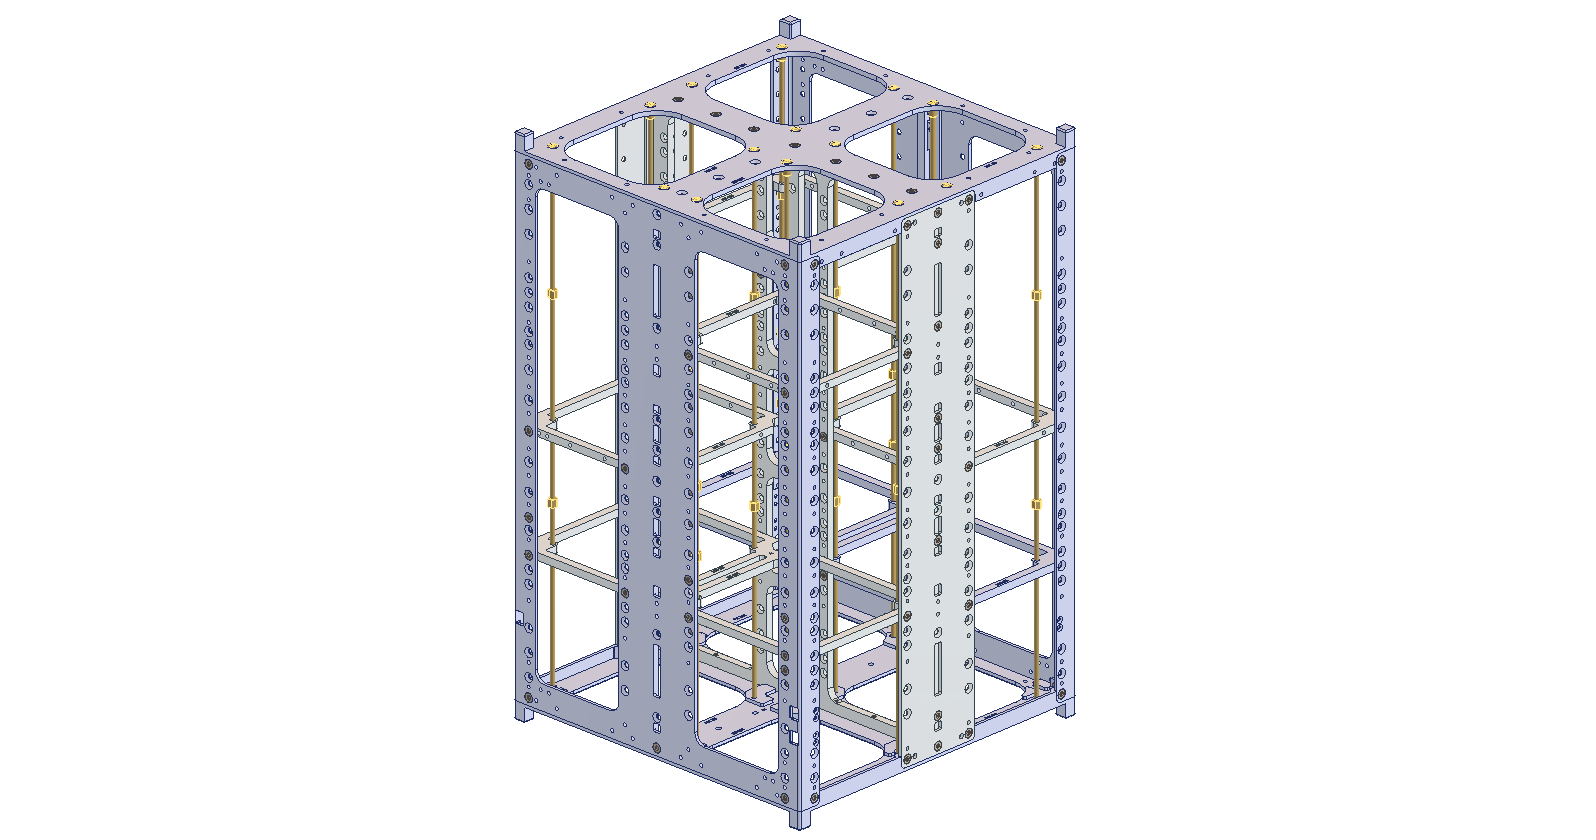
\includegraphics[width=0.85\linewidth]{PUCP_pictures/EnduroSat 12U CubeSat satellite model.png}
    \caption{Commercial 12U CubeSat reference model used as the geometric basis for the SAT-A configuration.}
    \label{fig:structural_endurosat_12u_model}
\end{figure}

The SAT-A model includes representative CubeSat subsystems, such as the On-Board Computer (OBC), Electrical Power System (EPS), UHF and S-band communications subsystems, solar panels, and an ADCS module. These elements were included to verify subsystem accommodation and to evaluate the remaining volume available for the SAT-BC payload. The main bus subsystems and ADCS module are placed in the lower region of SAT-A, while the upper internal volume is reserved for the SAT-BC assembly and its deployment path. This arrangement keeps the payload close to the deployment face from which SAT-BC is intended to be released.

Figure~\ref{fig:structural_sata_model} shows the external and internal views of the SAT-A CAD model. At this stage, the model verifies the geometric feasibility of accommodating the basic CubeSat subsystems, the ADCS module, and the SAT-BC payload within the 12U envelope. However, it has not yet been optimized for structural stiffness, launch-load compatibility, or final deployment-mechanism integration.

\begin{figure}[htbp]
    \centering
    \begin{subfigure}{0.42\textwidth}
        \centering
        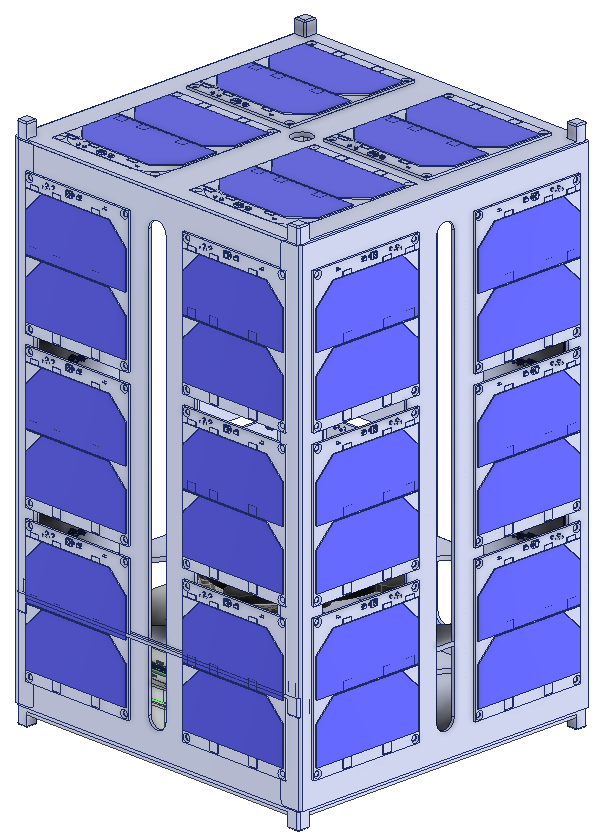
\includegraphics[width=\linewidth]{PUCP_pictures/External model of the SATA.png}
        \caption{External view.}
        \label{fig:structural_sata_external}
    \end{subfigure}
    \hfill
    \begin{subfigure}{0.40\textwidth}
        \centering
        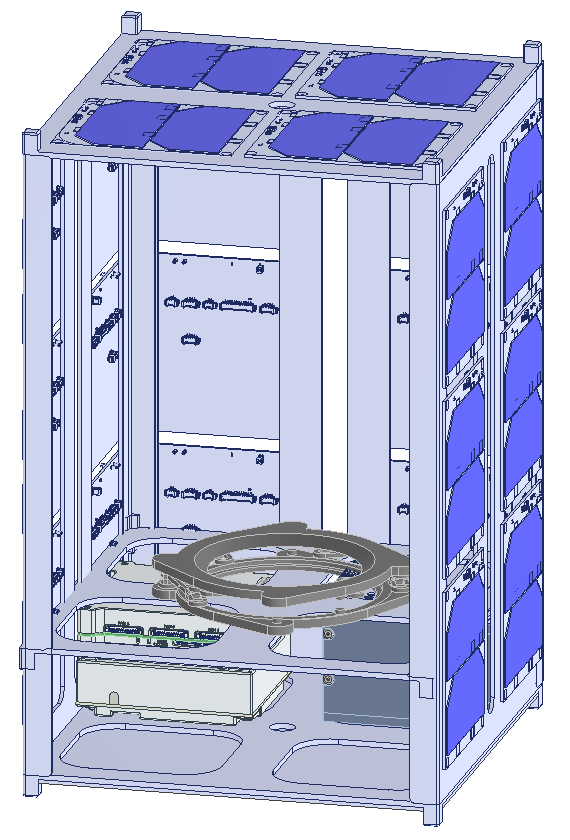
\includegraphics[width=\linewidth]{PUCP_pictures/Internal model of the SATA.png}
        \caption{Internal layout.}
        \label{fig:structural_sata_internal}
    \end{subfigure}
    \caption{SAT-A CAD model:
    (a) external configuration;
    (b) internal subsystem and payload accommodation.}
    \label{fig:structural_sata_model}
\end{figure}

The current SAT-A model should therefore be interpreted as an accommodation and layout model. Future iterations must incorporate additional structural elements, payload retention interfaces, and deployment-support features to improve stiffness and to support the controlled release of the SAT-BC assembly.

\subsection{SAT-B Configuration}
\label{sub:structural_satb}

SAT-B is a non-standard small-satellite structure designed to approximate a spherical body with a diameter of approximately \(20~\mathrm{cm}\). Since manufacturing a fully spherical structure would introduce significant complexity, the preliminary design approximates the spherical envelope using a dodecahedral geometry. This approach provides a more manufacturable structure while preserving an approximately isotropic external shape for the tethered-satellite concept.

The SAT-B structure is divided into three main modules: an upper module, a central module, and a lower module, as shown in Figure~\ref{fig:structural_satb_simplified_model}. This modular division supports the separation of mechanical functions and subsystem accommodation within the limited internal volume of the satellite.

\begin{figure}[htbp]
    \centering
    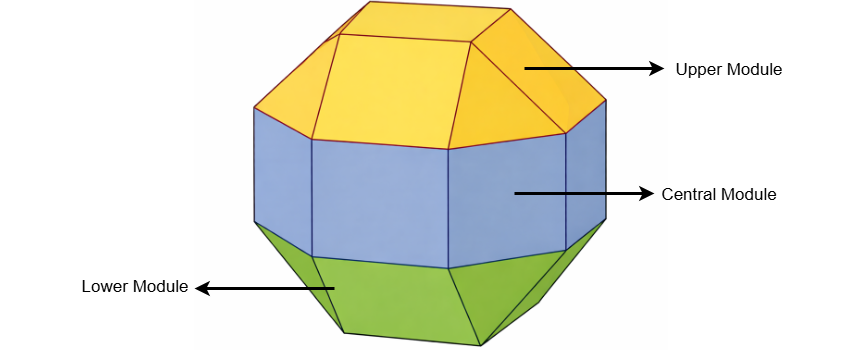
\includegraphics[width=0.85\linewidth]{PUCP_pictures/Simplified model of the SATB structure.png}
    \caption{Simplified modular representation of the SAT-B structure.}
    \label{fig:structural_satb_simplified_model}
\end{figure}

The upper module contains the main elements associated with the tether deployment and SAT-B/SAT-C separation functions. These include the tether spool, the tether routing elements, the force sensor interface, the spring-based deployment platform, the deployment guides, and the Arducam camera assemblies used to observe the tether from the SAT-B perspective. The tether spool is intended to store approximately \(100~\mathrm{m}\) of tether, while the force sensor interface provides a mechanical path for measuring tether tension at the SAT-B end. The deployment platform and guide elements are arranged to promote an axial separation between SAT-B and SAT-C and to reduce lateral disturbances during the initial deployment process.

The central module forms the main structural core of SAT-B. It is based on octagonal platforms connected by structural rails, producing an octagonal-prism arrangement that supports the overall dodecahedral geometry. This module accommodates representative electronic subsystems, including the On-Board Computer (OBC) and the Electrical Power System (EPS). As in the SAT-A model, commercial subsystem CAD models were used as geometric references to verify internal accommodation at this preliminary design stage.

The lower module is reserved for the integration of attitude-control and communication elements. In the current configuration, this region is intended to accommodate the magnetorquer assembly required for magnetic attitude-control functions and the UHF and S-band communications subsystems. These elements have not yet been fully detailed in the CAD model and must be incorporated in future structural iterations.

Figure~\ref{fig:structural_satb_central_module} shows the central structural module and the representative internal subsystem accommodation. These elements define the main load-bearing region of SAT-B and provide the mechanical interface for the upper and lower modules.

\begin{figure}[htbp]
    \centering
    \begin{subfigure}{0.48\textwidth}
        \centering
        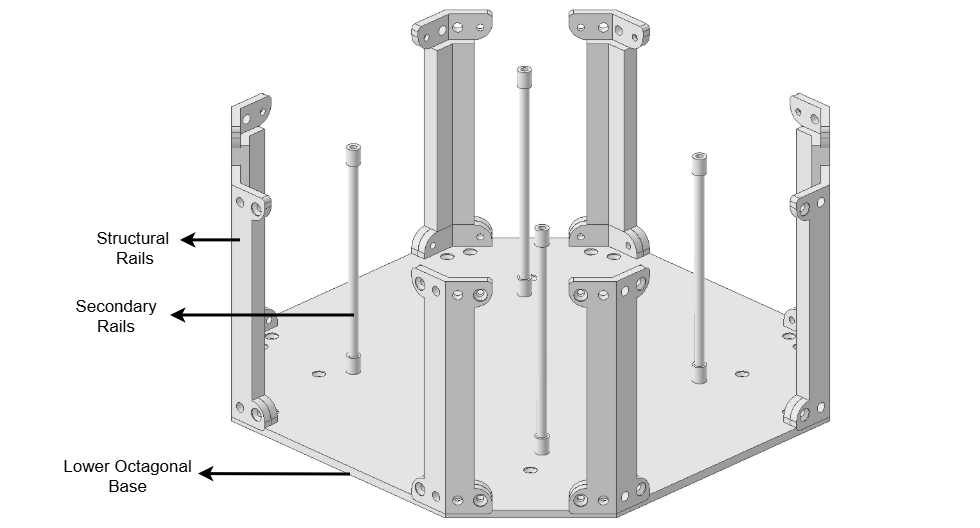
\includegraphics[width=\linewidth]{PUCP_pictures/Structure of the SATB central module (2).png}
        \caption{Central structural module.}
        \label{fig:structural_satb_central_structure}
    \end{subfigure}
    \hfill
    \begin{subfigure}{0.45\textwidth}
        \centering
        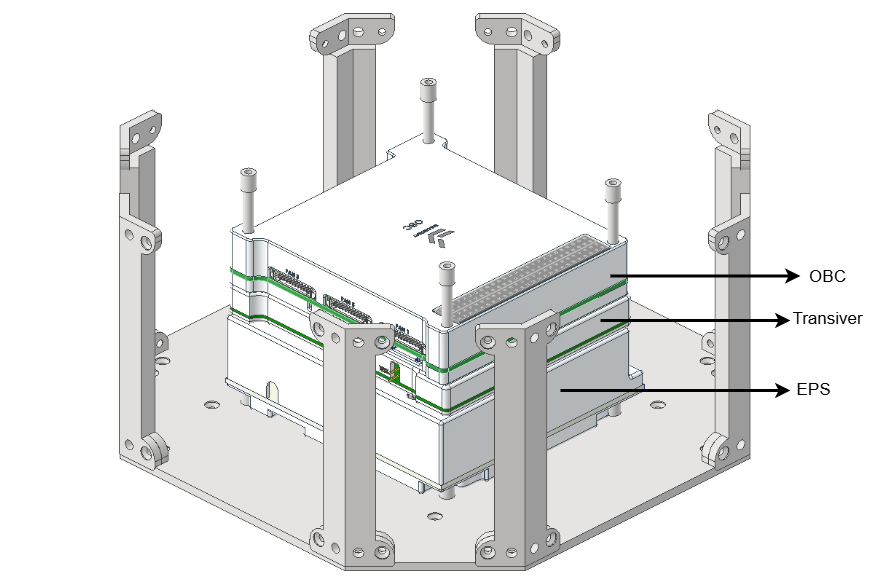
\includegraphics[width=\linewidth]{PUCP_pictures/Internal components of the SATB central module.png}
        \caption{Representative internal components.}
        \label{fig:structural_satb_internal_components}
    \end{subfigure}
    \caption{SAT-B central module:
    (a) structural rails and octagonal platforms;
    (b) accommodation of representative electronic subsystems.}
    \label{fig:structural_satb_central_module}
\end{figure}

Figure~\ref{fig:structural_satb_tether_deployment_elements} summarizes the main tether-deployment elements located in the SAT-B upper module. These elements define the mechanical path of the tether from the storage spool to the force sensor and separation platform.

\begin{figure}[htbp]
    \centering
    \begin{subfigure}{0.45\textwidth}
        \centering
        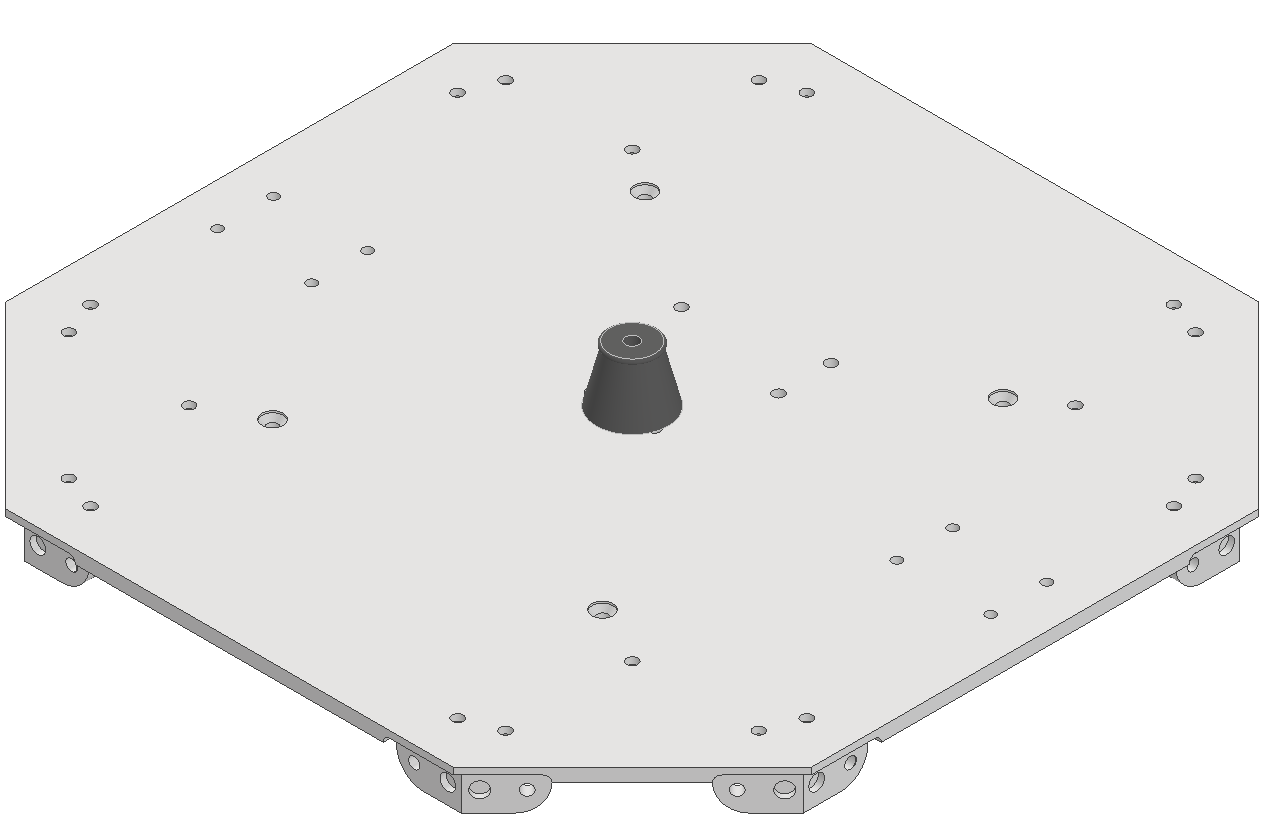
\includegraphics[width=\linewidth]{PUCP_pictures/Assembly of the upper octagonal base of the SATB with the Kevlar thread spool.png}
        \caption{Tether spool integration.}
        \label{fig:structural_satb_spool_integration}
    \end{subfigure}
    \hfill
    \begin{subfigure}{0.45\textwidth}
        \centering
        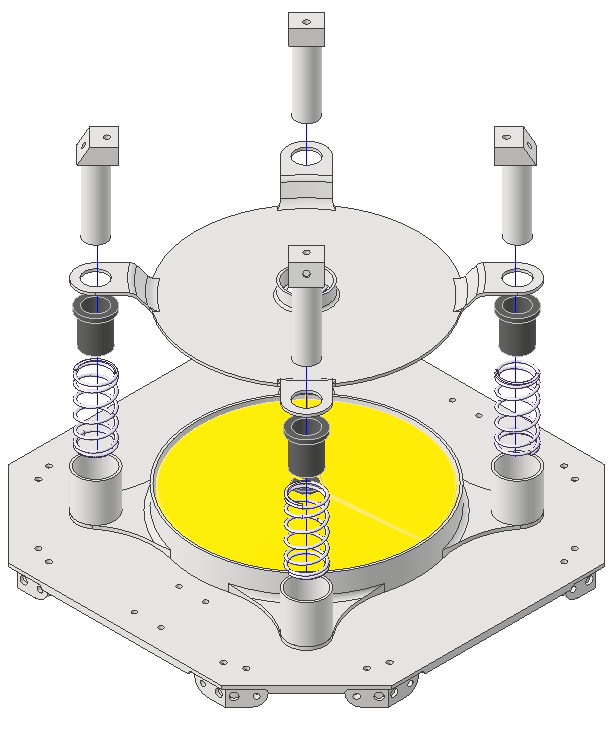
\includegraphics[width=\linewidth]{PUCP_pictures/Assembly of the SATB separation platform.png}
        \caption{Separation platform.}
        \label{fig:structural_satb_separation_platform}
    \end{subfigure}
    \caption{Representative tether-deployment elements in the SAT-B upper module:
    (a) tether spool;
    (b) spring-based separation platform.}
    \label{fig:structural_satb_tether_deployment_elements}
\end{figure}

The external faces of SAT-B are formed by inclined panels attached to angular brackets, allowing the structure to approximate the intended dodecahedral envelope. Several of these faces are used as mounting surfaces for solar panels. Commercial panels are considered where the available area allows their integration, while custom solar-cell assemblies are expected for smaller or non-standard faces. The upper cover includes a central opening that acts as a guide for the SAT-C ejection path, making this region a critical mechanical interface for the SAT-B/SAT-C separation event.

Figure~\ref{fig:structural_satb_complete_model} shows the complete SAT-B CAD model. At this stage, the model demonstrates the feasibility of accommodating the main structural modules, representative electronic subsystems, tether-storage elements, separation hardware, camera assemblies, and external solar-panel surfaces within the approximate spherical envelope. However, the model remains preliminary and requires further refinement of the magnetorquer accommodation, antenna integration, detailed fastening strategy, structural stiffness, and manufacturing constraints.

\begin{figure}[htbp]
    \centering
    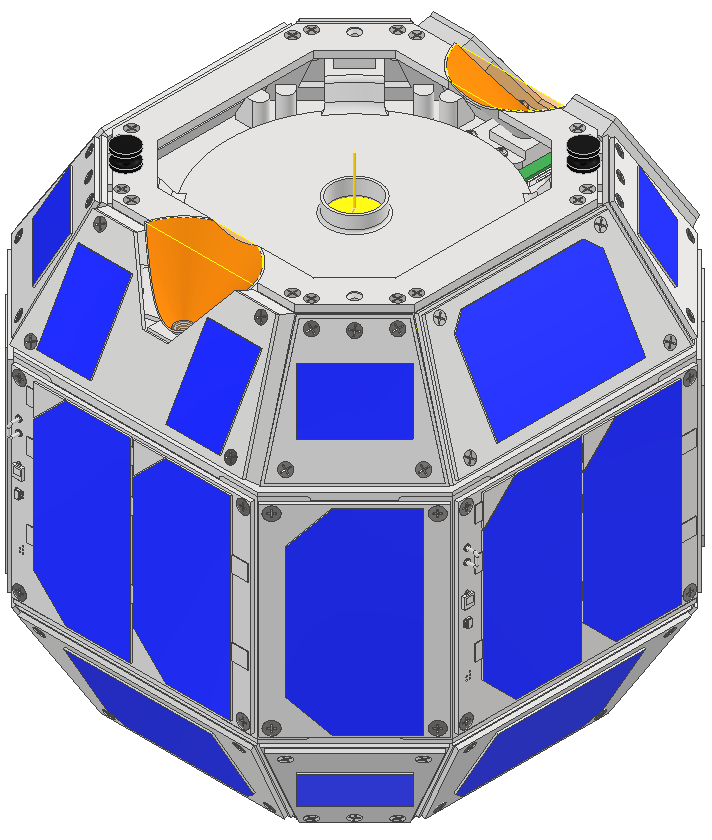
\includegraphics[width=0.48\linewidth]{PUCP_pictures/Complete CAD model of the SATB.png}
    \caption{CAD model of SAT-B.}
    \label{fig:structural_satb_complete_model}
\end{figure}

\subsection{SAT-C and SAT-BC Coupled Configuration}
\label{sub:structural_satc_satbc}

SAT-C is a non-standard small-satellite structure intended to approximate a spherical body with a diameter of approximately \(10~\mathrm{cm}\). As in the case of SAT-B, the spherical envelope is approximated using a dodecahedral geometry to simplify manufacturing and assembly while preserving the compact external shape required for the tethered-satellite concept. Due to its reduced size, SAT-C has internal-volume constraints comparable to a 1U CubeSat but does not follow a conventional CubeSat structural layout.

The SAT-C structure is organized into three main modules: a lower module, a central module, and an upper module. The lower module accommodates the SAT-C camera, the force sensor associated with the SAT-C end of the tether, the tether-routing elements, and the S-band antenna. The camera is intended to observe the tether from the SAT-C perspective, while the force sensor provides a redundant measurement of tether tension. The tether-routing elements, such as pulleys and guides, define the mechanical path of the tether between SAT-B and SAT-C. The S-band antenna is located in this module to provide the external communication interface with SAT-B required for data transmission.

The central module contains the locking and release elements associated with the SAT-B/SAT-C separation mechanism. In this region, the nylon retention thread is routed through internal guides and through the thermal cutting module. This thread keeps SAT-B and SAT-C mechanically coupled before separation. Once the thermal cutting mechanism is activated, the retention condition is released and the SAT-B/SAT-C separation sequence can begin. The central module must also accommodate the main electronic subsystems, including the On-Board Computer (OBC), Electrical Power System (EPS), and S-band transceiver. However, because of the limited internal volume of SAT-C, these components are expected to require custom designs rather than standard commercial CubeSat modules.

The upper module accommodates the GNSS receiver and its corresponding antenna, which support position and timing information for the reconstruction of the tethered-system motion. At the current design stage, the three-dimensional models of all components in this module are not yet fully defined. Therefore, the SAT-C CAD model should be interpreted as a preliminary accommodation and interface model rather than a final manufacturing configuration. Figure~\ref{fig:structural_satc_lower_module} summarizes the main elements of the SAT-C lower module, including the tether-routing and sensing interfaces.

\begin{figure}[htbp]
    \centering
    \begin{subfigure}{0.45\textwidth}
        \centering
        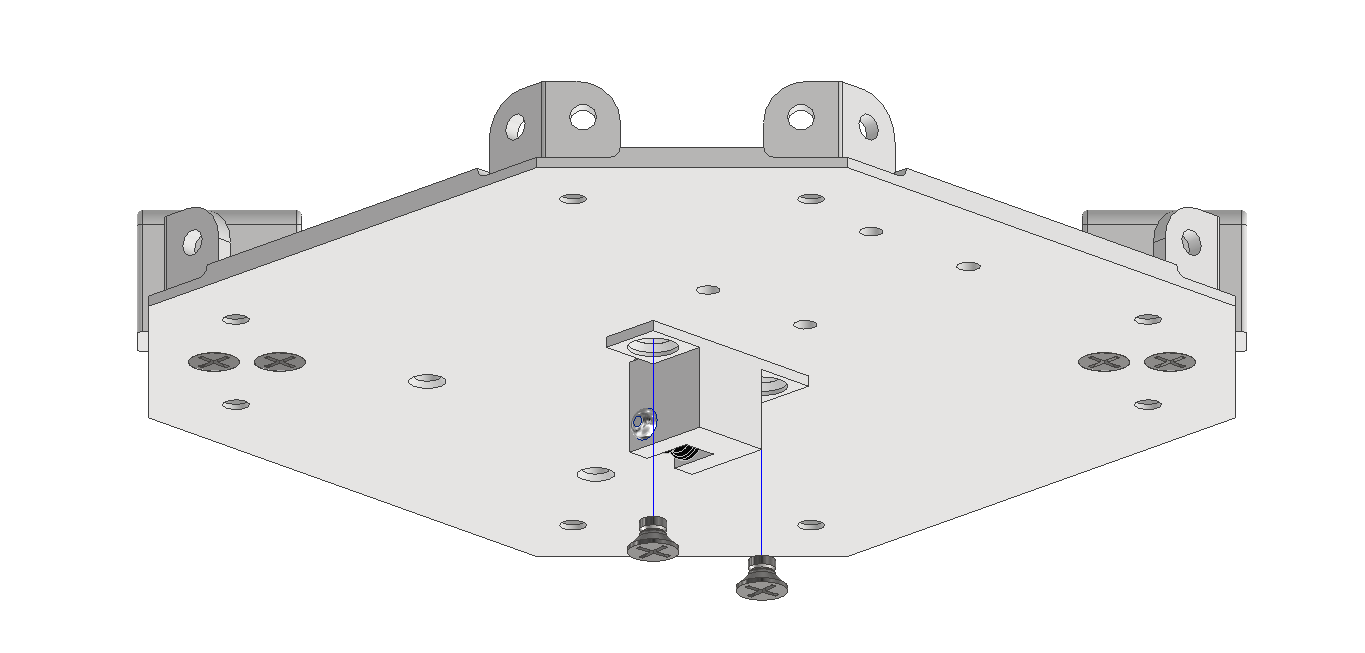
\includegraphics[width=\linewidth]{PUCP_pictures/Assembly of the pulley with the lower octagonal base of the SATC.png}
        \caption{Pulley and tether-routing interface.}
        \label{fig:structural_satc_pulley_interface}
    \end{subfigure}
    \hfill
    \begin{subfigure}{0.45\textwidth}
        \centering
        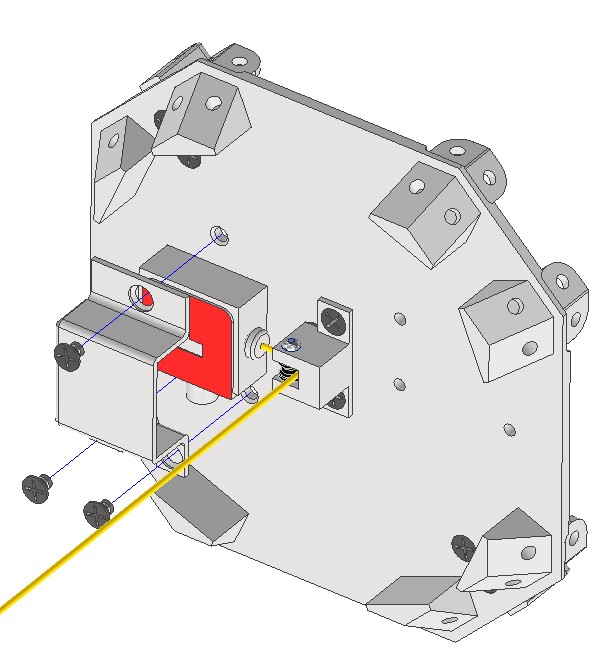
\includegraphics[width=\linewidth]{PUCP_pictures/Assembly of the force sensor in the SATC.png}
        \caption{Force sensor integration.}
        \label{fig:structural_satc_force_sensor}
    \end{subfigure}
    \caption{Representative SAT-C lower-module interfaces:
    (a) tether-routing pulley;
    (b) force sensor integration at the SAT-C tether end.}
    \label{fig:structural_satc_lower_module}
\end{figure}

The external faces of SAT-C are formed by inclined panels attached to angular brackets, following the same general design logic used for SAT-B. Several of these faces are used as mounting surfaces for solar panels. Since many SAT-C faces do not provide enough area for standard commercial panels, custom solar-cell assemblies are expected for the inclined and central faces. In addition, two central faces require openings to allow the nylon retention thread to pass from the SAT-C interior toward the locking pulleys located on SAT-B.

Figure~\ref{fig:structural_satc_external_modules} shows representative assemblies of the SAT-C lower and upper modules with inclined faces and solar-panel surfaces.

\begin{figure}[htbp]
    \centering
    \begin{subfigure}{0.47\textwidth}
        \centering
        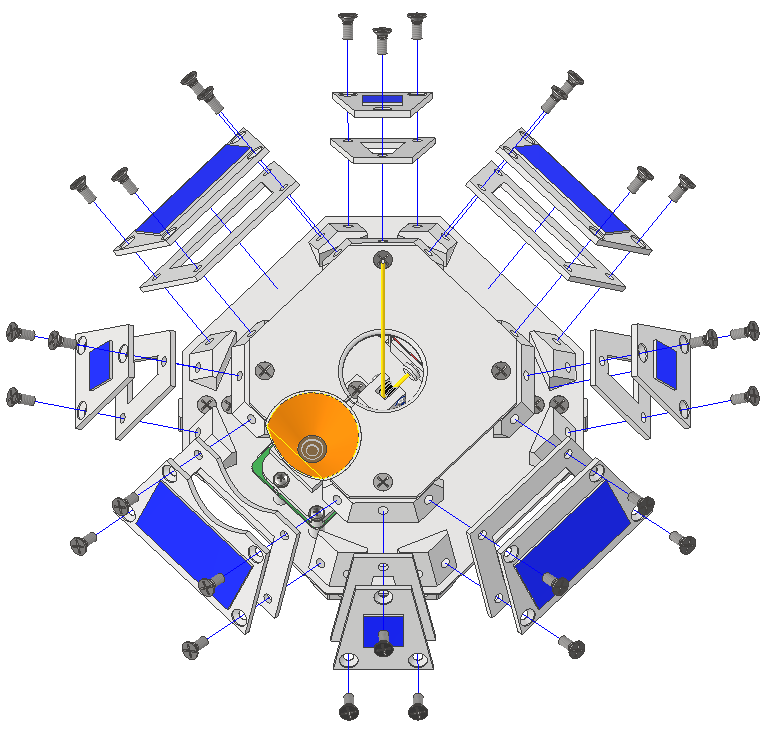
\includegraphics[width=\linewidth]{PUCP_pictures/Assembly of the inclined faces and solar panels in the SATC lower module.png}
        \caption{Lower module.}
        \label{fig:structural_satc_lower_faces}
    \end{subfigure}
    \hfill
    \begin{subfigure}{0.47\textwidth}
        \centering
        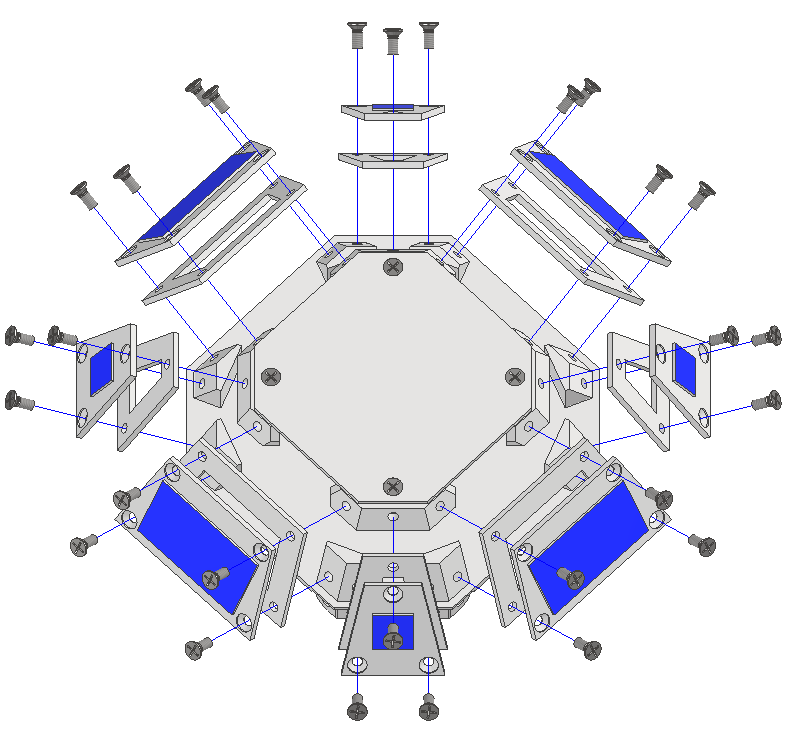
\includegraphics[width=\linewidth]{PUCP_pictures/Assembly of the inclined faces and solar panels in the SATC upper module.png}
        \caption{Upper module.}
        \label{fig:structural_satc_upper_faces}
    \end{subfigure}
    \caption{Representative SAT-C external module assemblies:
    (a) lower module with inclined faces and solar-panel surfaces;
    (b) upper module with inclined faces and solar-panel surfaces.}
    \label{fig:structural_satc_external_modules}
\end{figure}

The SAT-BC coupled configuration is formed when SAT-C is inserted into the corresponding guide region of SAT-B. In this configuration, SAT-B and SAT-C remain mechanically coupled and behave as a single payload assembly before the internal SAT-B/SAT-C separation command. The coupling relies on the nylon retention thread, which passes through the guides inside the SAT-C central module, through the thermal cutting module, and around the locking pulleys located on the SAT-B upper cover. This arrangement keeps the two satellites attached before deployment while preserving a defined release path for SAT-C.

Figure~\ref{fig:structural_satbc_coupled_model} shows the complete SAT-BC assembly. At this stage, the coupled model verifies the geometric compatibility between SAT-B and SAT-C, the feasibility of inserting SAT-C into the SAT-B guide region, and the routing of the tether and retention-thread interfaces. Further work is required to refine the separation mechanism, verify the retention and release loads, define detailed tolerances, and confirm that the coupled assembly can be stored and released from SAT-A without interference.

\begin{figure}[htbp]
    \centering
    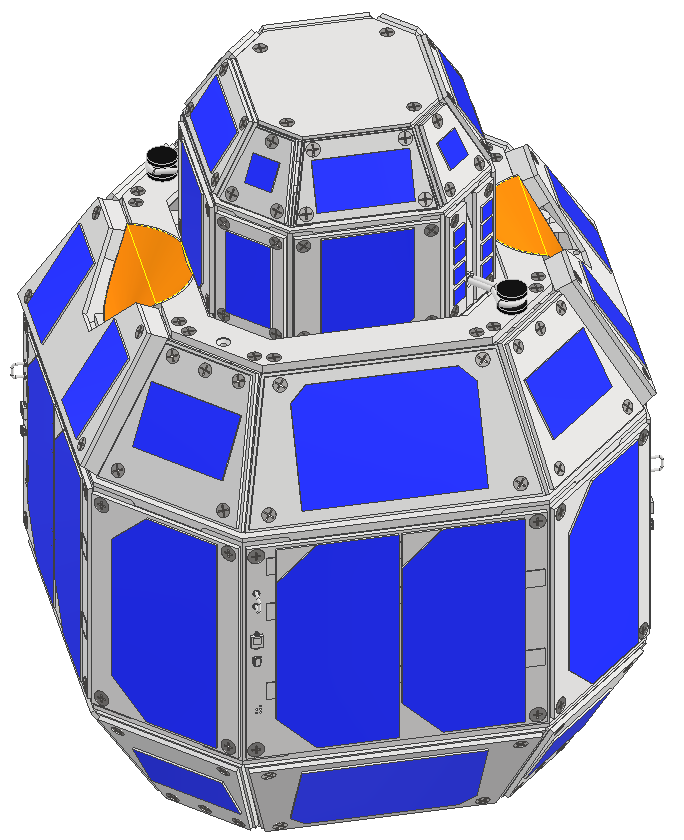
\includegraphics[width=0.62\linewidth]{PUCP_pictures/Complete assembly of the SATB with the SATC.png}
    \caption{CAD model of the coupled SAT-BC configuration.}
    \label{fig:structural_satbc_coupled_model}
\end{figure}

\newpage
\subsection{Preliminary Modal Analysis}
\label{sub:structural_modal_analysis}

A modal analysis was performed for the SAT-B structure, the SAT-C structure, and the coupled SAT-BC assembly using ANSYS and the Finite Element Method (FEM). The objective of this analysis is to identify the first natural frequencies and their associated mode shapes, providing an initial indication of the dynamic behavior of the proposed structural concepts.

The analysis was carried out using simplified CAD models. Measurement components, secondary mechanisms, detailed subsystem models, and small fastening elements such as bolts were omitted to avoid excessive mesh refinement at this stage. Each model was imported into ANSYS as a single solid body, assuming that the structural components behave as a continuous body. This approximation is suitable for an SRR-level assessment, but it does not replace a detailed structural model including contact definitions, fasteners, material interfaces, final assembly tolerances, and launcher-specific mechanical requirements.

\textbf{SAT-C modal analysis.}
For the SAT-C model, a simplified structure was used without measurement components and secondary mechanisms, such as the thermal cutting module. The mesh element size was set to \(0.5~\mathrm{mm}\), considering that some regions of the SAT-C structure have characteristic dimensions close to \(1\)--\(2~\mathrm{mm}\). The resulting mesh quality was approximately \(73.7\%\), as shown in Figure~\ref{fig:structural_modal_satc_mesh}.

After the mesh was generated, a fixed support condition was applied at the base of SAT-C, as shown in Figure~\ref{fig:structural_modal_satc_support}. This boundary condition constrains the lower region of the model and provides a reference condition for identifying the vibration modes. Since this constraint is idealized, the resulting natural frequencies should be interpreted as preliminary indicators rather than final qualification values.

Using this simplified model, the first ten vibration modes of the SAT-C structure were computed. The first natural frequency was \(468.64~\mathrm{Hz}\). For this mode, the largest modal deformation was concentrated in the upper module, which is the region farthest from the fixed support. The corresponding modal deformation result is shown in Figure~\ref{fig:structural_modal_satc_result}.

\begin{figure}[H]
    \centering
    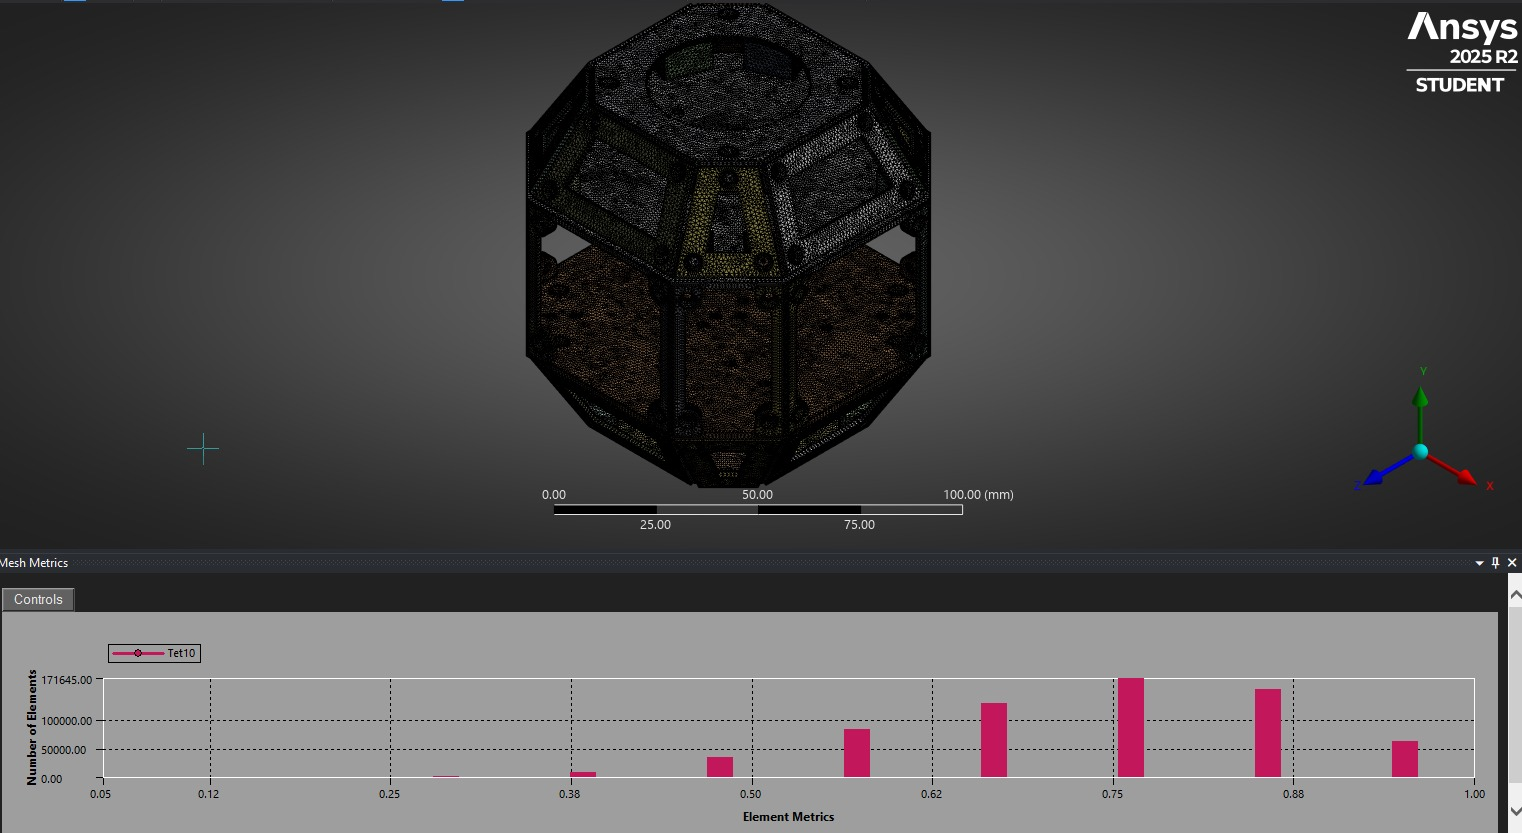
\includegraphics[width=\linewidth,height=8cm,keepaspectratio]{PUCP_pictures/0.5 mm element mesh for the simplified SAT-C model.jpeg}
    \caption{Finite-element mesh of the simplified SAT-C model with a \(0.5~\mathrm{mm}\) element size.}
    \label{fig:structural_modal_satc_mesh}
\end{figure}

\begin{figure}[H]
    \centering
    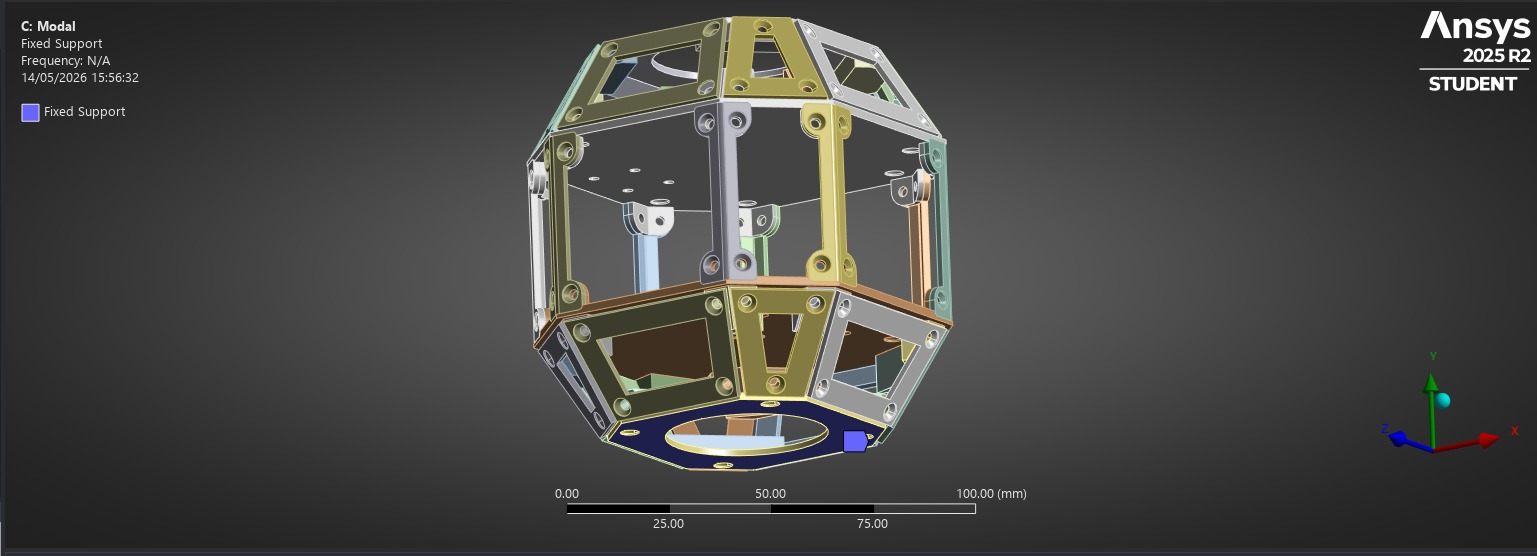
\includegraphics[width=\linewidth,height=8cm,keepaspectratio]{PUCP_pictures/Fixed support condition of the SAT-C for the modal analysis.jpeg}
    \caption{Fixed support condition applied to the simplified SAT-C model.}
    \label{fig:structural_modal_satc_support}
\end{figure}

\begin{figure}[H]
    \centering
    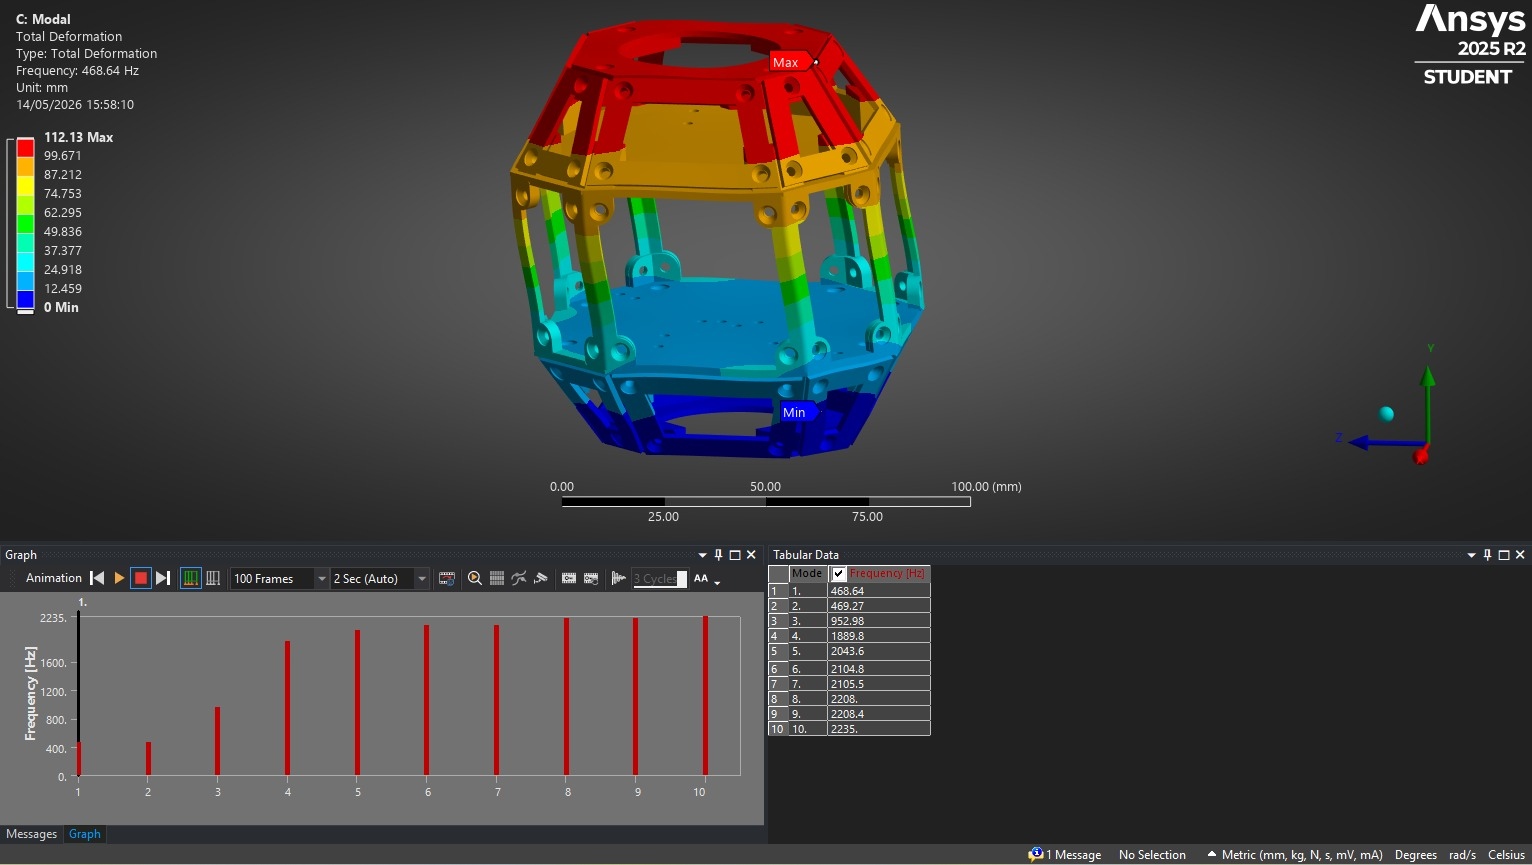
\includegraphics[width=\linewidth,height=8cm,keepaspectratio]{PUCP_pictures/Results of the first ten vibration modes for the SAT-C structure.jpeg}
    \caption{Modal deformation result for the first natural frequency of the simplified SAT-C model.}
    \label{fig:structural_modal_satc_result}
\end{figure}


\textbf{SAT-B modal analysis.}
For the SAT-B model, a simplified structure was used. The model excluded the detailed internal subsystems located in the central module, the force sensor, the camera assemblies, small fastening elements, and detailed separation-mechanism features. The mesh element size was set to \(1~\mathrm{mm}\), considering the larger dimensions of SAT-B and the level of geometric detail required for this preliminary assessment. The resulting mesh quality was approximately \(72.5\%\), as shown in Figure~\ref{fig:structural_modal_satb_mesh}.

After the mesh was generated, a fixed support condition was applied at the base of the SAT-B lower module, as shown in Figure~\ref{fig:structural_modal_satb_support}. This boundary condition follows the same modeling approach used for SAT-C and provides a consistent reference for comparing the modal behavior of both individual satellite structures.

Using this simplified model, the first six vibration modes of the SAT-B structure were computed. The first natural frequency was \(302.83~\mathrm{Hz}\). The largest modal deformation for this mode was concentrated in the upper module, similar to the SAT-C case, because this region is farthest from the fixed support. The lower first natural frequency compared with SAT-C is consistent with the larger size and lower relative stiffness of the SAT-B configuration. The corresponding modal deformation result is shown in Figure~\ref{fig:structural_modal_satb_result}.

\begin{figure}[H]
    \centering
    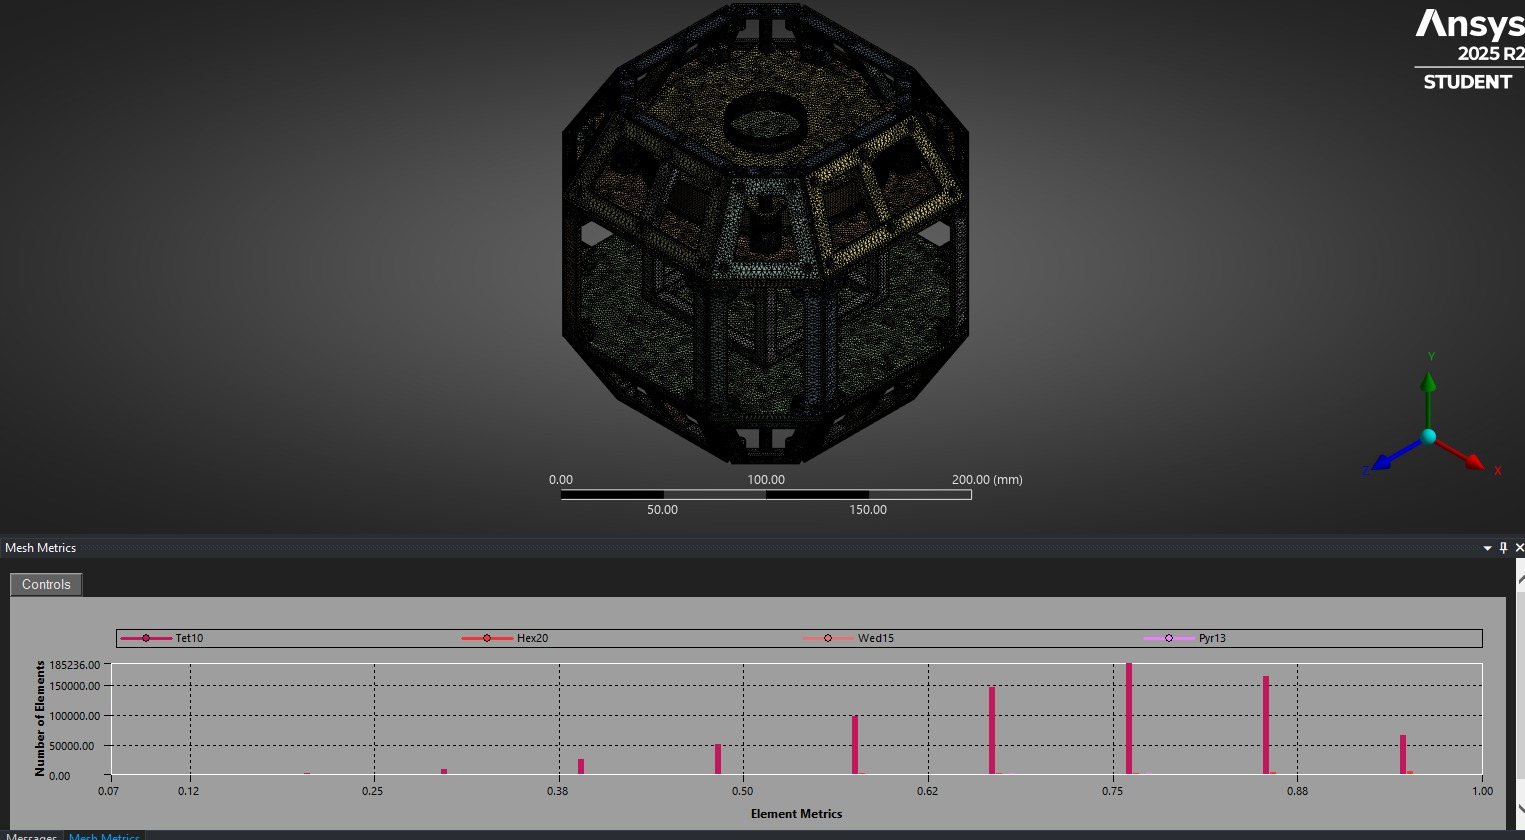
\includegraphics[width=\linewidth,height=8cm,keepaspectratio]{PUCP_pictures/1 mm element mesh for the simplified SAT-B model.jpeg}
    \caption{Finite-element mesh of the simplified SAT-B model with a \(1~\mathrm{mm}\) element size.}
    \label{fig:structural_modal_satb_mesh}
\end{figure}

\begin{figure}[H]
    \centering
    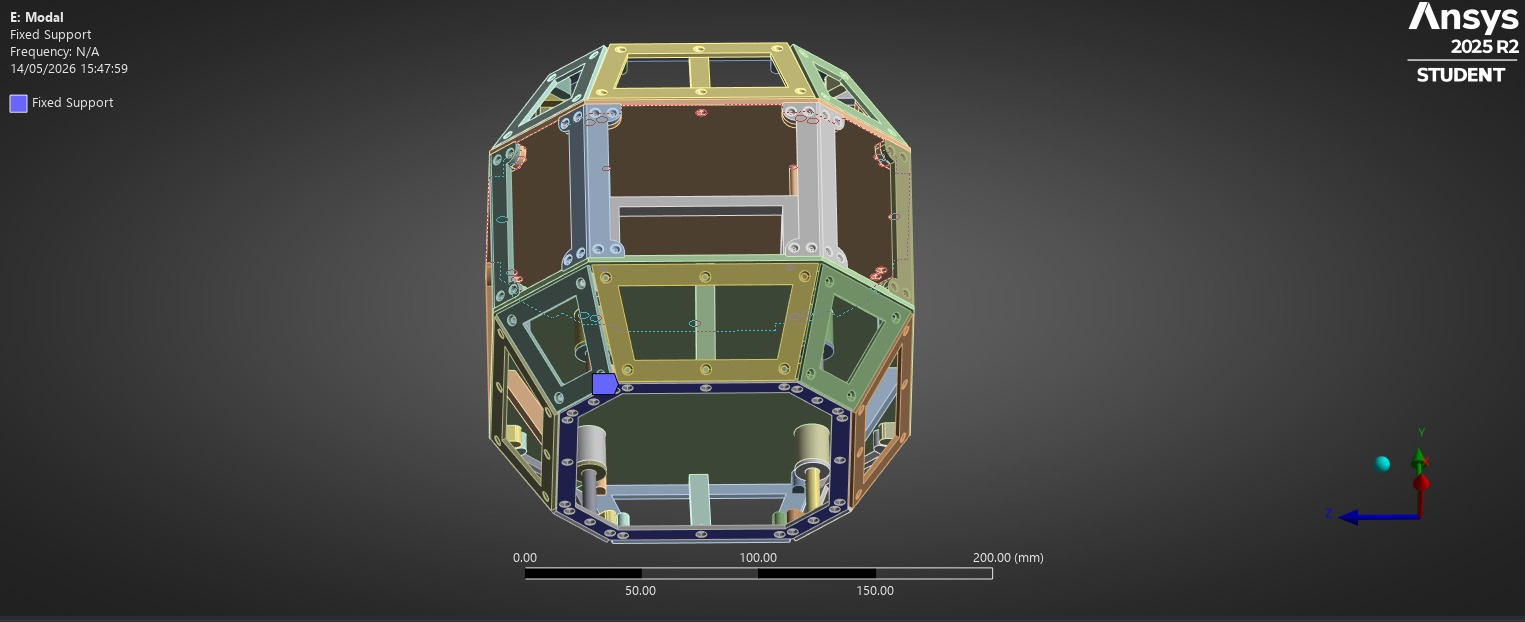
\includegraphics[width=\linewidth,height=8cm,keepaspectratio]{PUCP_pictures/Fixed support condition of the SAT-B for the modal analysis.jpeg}
    \caption{Fixed support condition applied to the simplified SAT-B model.}
    \label{fig:structural_modal_satb_support}
\end{figure}

\begin{figure}[H]
    \centering
    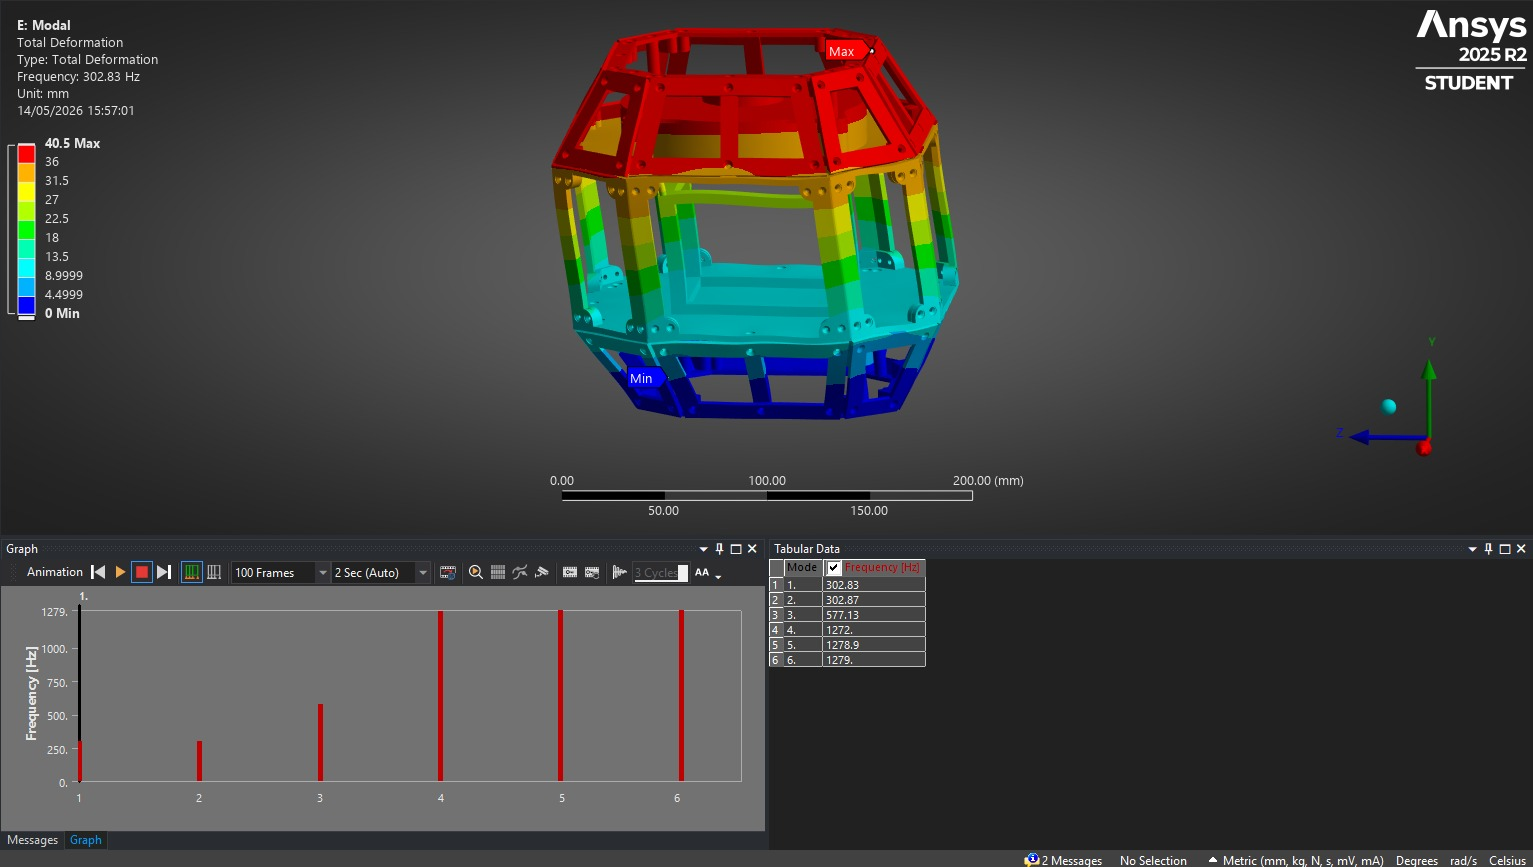
\includegraphics[width=\linewidth,height=8cm,keepaspectratio]{PUCP_pictures/Results of the first six vibration modes for the SAT-B structure.jpeg}
    \caption{Modal deformation result for the first natural frequency of the simplified SAT-B model.}
    \label{fig:structural_modal_satb_result}
\end{figure}


\textbf{SAT-BC modal analysis.}
For the coupled SAT-BC configuration, the simplified SAT-B and SAT-C models were integrated to evaluate the dynamic behavior of the combined assembly before SAT-B/SAT-C separation. The model was imported into ANSYS as a single solid body, assuming a continuous structural connection between the simplified SAT-B and SAT-C geometries. This assumption is useful for an initial comparison, but future analyses must include the actual mechanical interfaces, retention elements, contact conditions, and separation-mechanism details. The mesh element size was set to \(0.5~\mathrm{mm}\), using the smaller characteristic dimensions of SAT-C as the limiting reference. The resulting mesh quality was approximately \(74.3\%\), as shown in Figure~\ref{fig:structural_modal_satbc_mesh}.

After the mesh was generated, a fixed support condition was applied at the lower module of SAT-B, as shown in Figure~\ref{fig:structural_modal_satbc_support}. This condition constrains the base of the coupled assembly and allows the deformation behavior of the SAT-C region and the SAT-B/SAT-C interface to be observed in the modal results.

Using this simplified coupled model, the first four vibration modes of the SAT-BC assembly were computed. The first natural frequency was \(142.17~\mathrm{Hz}\), with the largest modal deformation concentrated in the SAT-C upper module. This value is lower than the first natural frequencies obtained for the individual SAT-B and SAT-C structures, indicating that the coupled SAT-BC configuration is more flexible in the simplified model. Particular attention must therefore be given to the SAT-B/SAT-C interface region in future analyses, since this region includes the separation mechanism and must maintain proper alignment and retention before deployment. The corresponding modal deformation result is shown in Figure~\ref{fig:structural_modal_satbc_result}.

\begin{figure}[H]
    \centering
    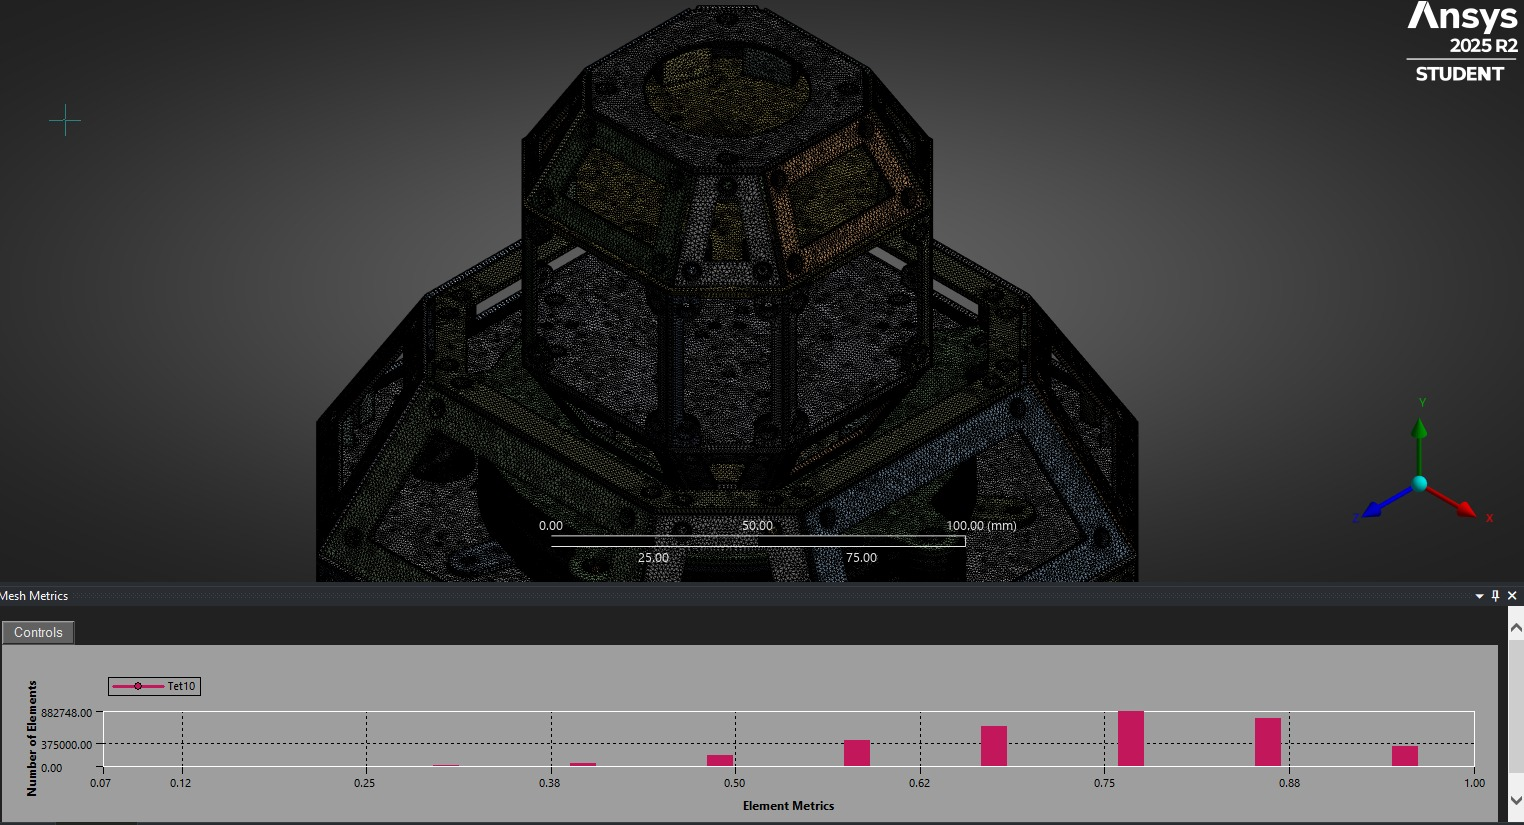
\includegraphics[width=\linewidth,height=8cm,keepaspectratio]{PUCP_pictures/0.5 mm element mesh for the simplified SAT-B - SAT-C model.jpeg}
    \caption{Finite-element mesh of the simplified coupled SAT-BC model with a \(0.5~\mathrm{mm}\) element size.}
    \label{fig:structural_modal_satbc_mesh}
\end{figure}

\begin{figure}[H]
    \centering
    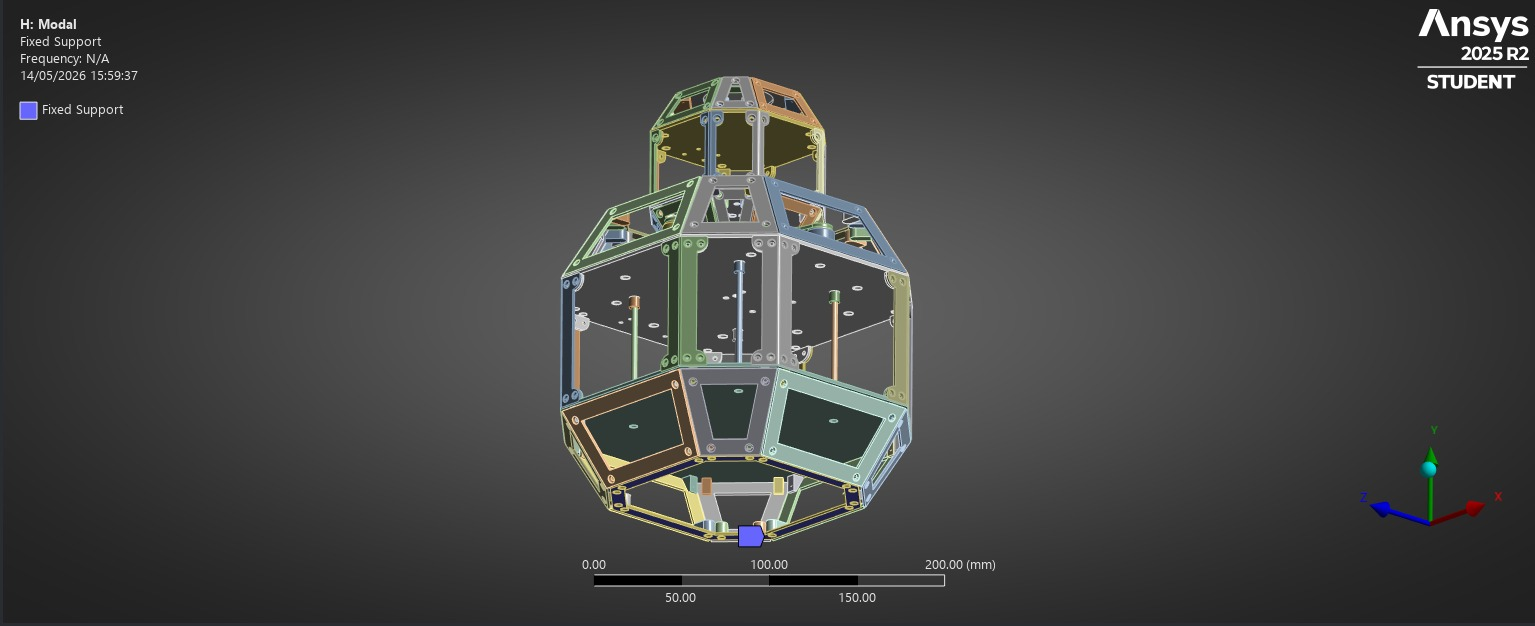
\includegraphics[width=\linewidth,height=8cm,keepaspectratio]{PUCP_pictures/Fixed support condition of the SAT-B - SAT-C for the modal analysis.jpeg}
    \caption{Fixed support condition applied to the simplified coupled SAT-BC model.}
    \label{fig:structural_modal_satbc_support}
\end{figure}

\begin{figure}[H]
    \centering
    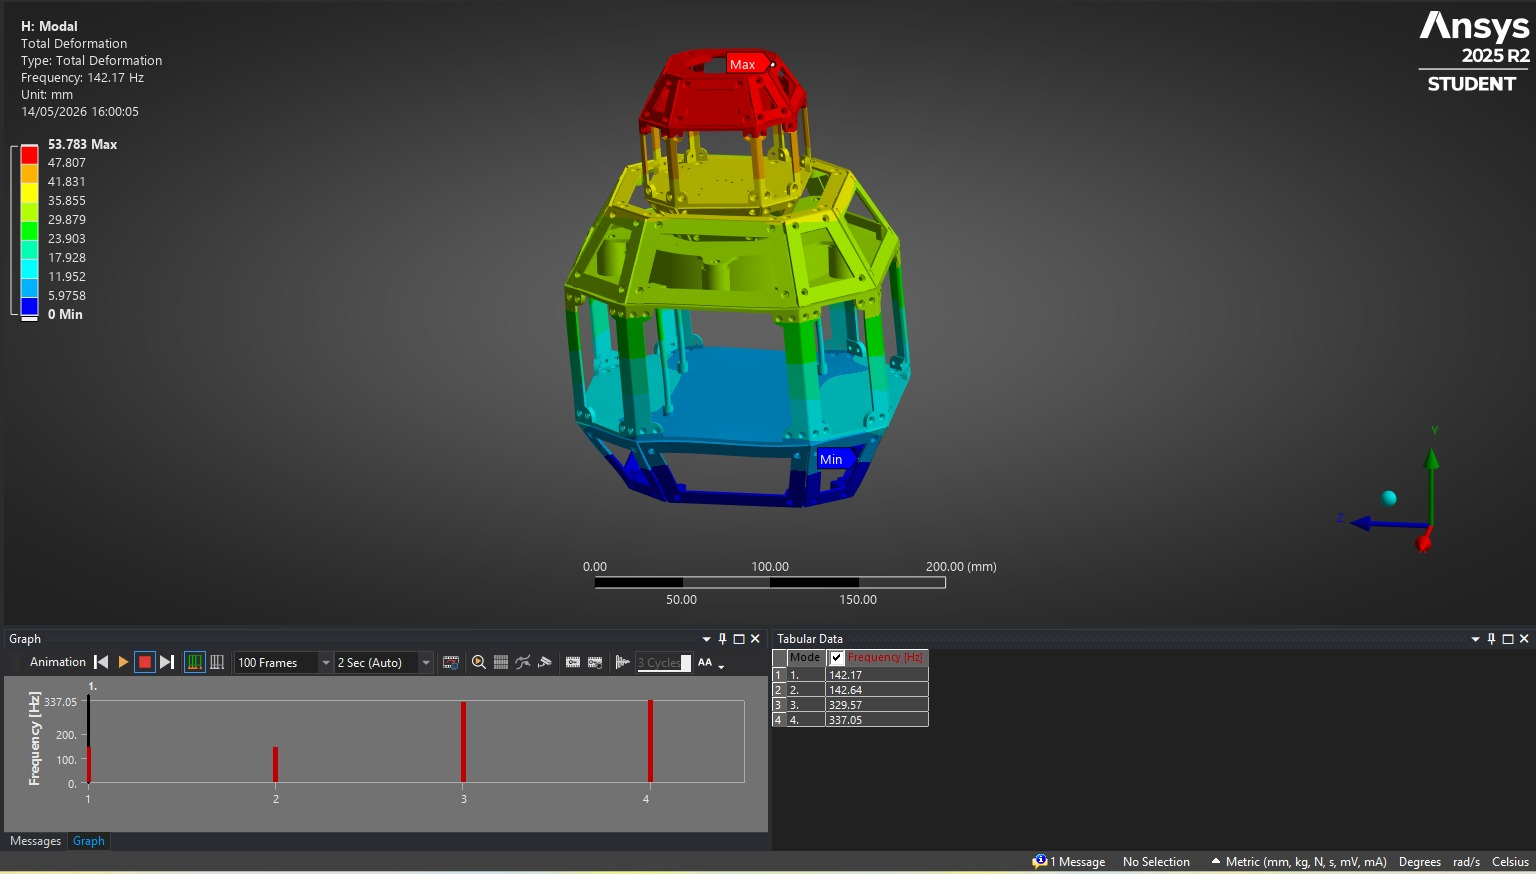
\includegraphics[width=\linewidth,height=8cm,keepaspectratio]{PUCP_pictures/Results of the first four vibration modes for the SAT-B - SAT-C structure.jpeg}
    \caption{Modal deformation result for the first natural frequency of the simplified coupled SAT-BC model.}
    \label{fig:structural_modal_satbc_result}
\end{figure}

The modal-analysis results are summarized in Table~\ref{tab:structural_modal_summary}. The values provide a first comparison of the dynamic behavior of the SAT-C, SAT-B, and SAT-BC structural models under the simplified assumptions described above. Therefore, they should be interpreted as preliminary design indicators and not as structural qualification results. 

For the next design iteration and ANSYS analysis, the structural model will be refined by replacing the current rigid body connections with explicit contact definitions. Localized Bonded or No-Separation contact conditions will be implemented at all bolted interfaces and mechanically fitted joints to more accurately represent the physical behavior of the assembly.

Furthermore, the next phase of the analysis will extend beyond the evaluation of the primary structures by incorporating the actual mechanical interfaces between the subsystems. This includes the integration of the Separation and Tether Deployment Mechanism described in Chapter 4, together with the associated locking system that maintains the springs in their compressed state. Consequently, the locked configuration of the separation system will be used to keep the SAT-B and SAT-C structures assembled throughout the simulation, providing a more realistic representation of the engineering model during launch and operational load cases.


%Future work must refine the structural models by including realistic interfaces, fasteners, material properties, contact conditions, and launcher-specific vibration requirements.

\begin{table}[htbp]
\centering
\caption{Summary of modal-analysis results for the SAT-C, SAT-B, and SAT-BC configurations.}
\label{tab:structural_modal_summary}
\begin{tabular}{lcccc}
\toprule
\textbf{Configuration} & \textbf{Mesh size} & \textbf{Mesh quality} & \textbf{Modes} & \textbf{First natural frequency} \\
 & \textbf{[mm]} & \textbf{[\%]} & \textbf{computed} & \textbf{[Hz]} \\
\midrule
SAT-C  & 0.5 & 73.7 & 10 & 468.64 \\
SAT-B  & 1.0 & 72.5 & 6  & 302.83 \\
SAT-BC & 0.5 & 74.3 & 4  & 142.17 \\
\bottomrule
\end{tabular}
\end{table}
